\documentclass{article}
%DIF LATEXDIFF DIFFERENCE FILE
%DIF DEL 2-main.tex   Wed Sep 20 17:14:25 2023
%DIF ADD 3-main.tex   Wed Nov 15 20:49:44 2023
\usepackage[utf8]{inputenc}
\usepackage{authblk}
\usepackage{setspace}
\usepackage[margin=1.25in]{geometry}
\usepackage{graphicx}
% \graphicspath{ {./figures/} }
\graphicspath{ {../figures/} }
%DIF 9a9
% \graphicspath{ {../../attachments} } %DIF > 
%DIF -------
\usepackage{subcaption} 
\usepackage{amsmath}
\usepackage{lineno}
\linenumbers

\usepackage{enumerate}
\DeclareMathOperator{\diag}{diag}
\usepackage{multirow}
\usepackage{booktabs}
\usepackage{footnote}
\usepackage{bm}
\usepackage[ruled,linesnumbered]{algorithm2e}
\setcounter{MaxMatrixCols}{20}
\usepackage{tikz}
\usetikzlibrary{arrows.meta, calc, fit, positioning, quotes, graphs, shapes.geometric}
\def\T{\mathrm{T}}

%%%%%% Bibliography %%%%%%
% Replace "sample" in the \addbibresource line below with the name of your .bib file.
% \usepackage[style=nejm, 
% citestyle=numeric-comp, 
% sorting=none]{biblatex}
% \addbibresource{ref.bib}

%%%%%% Title %%%%%%
% Full titles can be a maximum of 100 characters, including spaces. 
% Title Format: Use title case, capitalizing the first letter of each word, except for certain small words, such as articles and short prepositions
% \title{Using a Directed Graph Model and Greedy Algorithm to Determine the Maximum Allowable Current in a Reconfigurable Battery System}
%DIF 37c38
%DIF < \title{Maximum Allowable Current Determination of RBS By Using a Directed Graph Model and Greedy Algorithm}
%DIF -------
\title{Determining the Maximum Allowable Current of an RBS using a Directed Graph Model and Greedy Algorithm} %DIF > 
%DIF -------

%%%%%% Authors %%%%%%
% Authors should be listed in order of contribution to the paper, by first name, then middle initial (if any), followed by last name.
% Authors should be listed in the order in which they will appear in the published version if the manuscript is accepted. 
% Use an asterisk (*) to identify the corresponding author, and be sure to include that person’s e-mail address. Use symbols (in this order: †, ‡, §, ||, ¶, #, ††, ‡‡, etc.) for author notes, such as present addresses, “These authors contributed equally to this work” notations, and similar information.
% You can include group authors, but please include a list of the actual authors (the group members) in the Supplementary Materials.
\author[1$\dag$]{Binghui Xu}
\author[1$\dag$]{Guangbin Hua}
\author[1*]{Cheng Qian}
\author[1,2]{Quan Xia}
\author[1]{Bo Sun}
\author[1]{Yi Ren}
\author[1]{Zili Wang}

%%%%%% Affiliations %%%%%%
\affil[1]{School of Reliability and Systems Engineering, Beihang University, Beijing, 100191, China}
\affil[2]{School of Aeronautic Science and Engineering at Beihang University, Beijing, China}
\affil[*]{Address correspondence to: cqian@buaa.edu.cn}
\affil[$\dag$]{These authors contributed equally to this work.}

%%%%%% Date %%%%%%
% Date is optional
\date{}

%%%%%% Spacing %%%%%%
% Use paragraph spacing of 1.5 or 2 (for double spacing, use command \doublespacing)
\onehalfspacing
%DIF PREAMBLE EXTENSION ADDED BY LATEXDIFF
%DIF UNDERLINE PREAMBLE %DIF PREAMBLE
\RequirePackage[normalem]{ulem} %DIF PREAMBLE
\RequirePackage{color}\definecolor{RED}{rgb}{1,0,0}\definecolor{BLUE}{rgb}{0,0,1} %DIF PREAMBLE
\providecommand{\DIFadd}[1]{{\protect\color{blue}\uwave{#1}}} %DIF PREAMBLE
\providecommand{\DIFdel}[1]{{\protect\color{red}\sout{#1}}}                      %DIF PREAMBLE
%DIF SAFE PREAMBLE %DIF PREAMBLE
\providecommand{\DIFaddbegin}{} %DIF PREAMBLE
\providecommand{\DIFaddend}{} %DIF PREAMBLE
\providecommand{\DIFdelbegin}{} %DIF PREAMBLE
\providecommand{\DIFdelend}{} %DIF PREAMBLE
\providecommand{\DIFmodbegin}{} %DIF PREAMBLE
\providecommand{\DIFmodend}{} %DIF PREAMBLE
%DIF FLOATSAFE PREAMBLE %DIF PREAMBLE
\providecommand{\DIFaddFL}[1]{\DIFadd{#1}} %DIF PREAMBLE
\providecommand{\DIFdelFL}[1]{\DIFdel{#1}} %DIF PREAMBLE
\providecommand{\DIFaddbeginFL}{} %DIF PREAMBLE
\providecommand{\DIFaddendFL}{} %DIF PREAMBLE
\providecommand{\DIFdelbeginFL}{} %DIF PREAMBLE
\providecommand{\DIFdelendFL}{} %DIF PREAMBLE
\newcommand{\DIFscaledelfig}{0.5}
%DIF HIGHLIGHTGRAPHICS PREAMBLE %DIF PREAMBLE
\RequirePackage{settobox} %DIF PREAMBLE
\RequirePackage{letltxmacro} %DIF PREAMBLE
\newsavebox{\DIFdelgraphicsbox} %DIF PREAMBLE
\newlength{\DIFdelgraphicswidth} %DIF PREAMBLE
\newlength{\DIFdelgraphicsheight} %DIF PREAMBLE
% store original definition of \includegraphics %DIF PREAMBLE
\LetLtxMacro{\DIFOincludegraphics}{\includegraphics} %DIF PREAMBLE
\newcommand{\DIFaddincludegraphics}[2][]{{\color{blue}\fbox{\DIFOincludegraphics[#1]{#2}}}} %DIF PREAMBLE
\newcommand{\DIFdelincludegraphics}[2][]{% %DIF PREAMBLE
\sbox{\DIFdelgraphicsbox}{\DIFOincludegraphics[#1]{#2}}% %DIF PREAMBLE
\settoboxwidth{\DIFdelgraphicswidth}{\DIFdelgraphicsbox} %DIF PREAMBLE
\settoboxtotalheight{\DIFdelgraphicsheight}{\DIFdelgraphicsbox} %DIF PREAMBLE
\scalebox{\DIFscaledelfig}{% %DIF PREAMBLE
\parbox[b]{\DIFdelgraphicswidth}{\usebox{\DIFdelgraphicsbox}\\[-\baselineskip] \rule{\DIFdelgraphicswidth}{0em}}\llap{\resizebox{\DIFdelgraphicswidth}{\DIFdelgraphicsheight}{% %DIF PREAMBLE
\setlength{\unitlength}{\DIFdelgraphicswidth}% %DIF PREAMBLE
\begin{picture}(1,1)% %DIF PREAMBLE
\thicklines\linethickness{2pt} %DIF PREAMBLE
{\color[rgb]{1,0,0}\put(0,0){\framebox(1,1){}}}% %DIF PREAMBLE
{\color[rgb]{1,0,0}\put(0,0){\line( 1,1){1}}}% %DIF PREAMBLE
{\color[rgb]{1,0,0}\put(0,1){\line(1,-1){1}}}% %DIF PREAMBLE
\end{picture}% %DIF PREAMBLE
}\hspace*{3pt}}} %DIF PREAMBLE
} %DIF PREAMBLE
\LetLtxMacro{\DIFOaddbegin}{\DIFaddbegin} %DIF PREAMBLE
\LetLtxMacro{\DIFOaddend}{\DIFaddend} %DIF PREAMBLE
\LetLtxMacro{\DIFOdelbegin}{\DIFdelbegin} %DIF PREAMBLE
\LetLtxMacro{\DIFOdelend}{\DIFdelend} %DIF PREAMBLE
\DeclareRobustCommand{\DIFaddbegin}{\DIFOaddbegin \let\includegraphics\DIFaddincludegraphics} %DIF PREAMBLE
\DeclareRobustCommand{\DIFaddend}{\DIFOaddend \let\includegraphics\DIFOincludegraphics} %DIF PREAMBLE
\DeclareRobustCommand{\DIFdelbegin}{\DIFOdelbegin \let\includegraphics\DIFdelincludegraphics} %DIF PREAMBLE
\DeclareRobustCommand{\DIFdelend}{\DIFOaddend \let\includegraphics\DIFOincludegraphics} %DIF PREAMBLE
\LetLtxMacro{\DIFOaddbeginFL}{\DIFaddbeginFL} %DIF PREAMBLE
\LetLtxMacro{\DIFOaddendFL}{\DIFaddendFL} %DIF PREAMBLE
\LetLtxMacro{\DIFOdelbeginFL}{\DIFdelbeginFL} %DIF PREAMBLE
\LetLtxMacro{\DIFOdelendFL}{\DIFdelendFL} %DIF PREAMBLE
\DeclareRobustCommand{\DIFaddbeginFL}{\DIFOaddbeginFL \let\includegraphics\DIFaddincludegraphics} %DIF PREAMBLE
\DeclareRobustCommand{\DIFaddendFL}{\DIFOaddendFL \let\includegraphics\DIFOincludegraphics} %DIF PREAMBLE
\DeclareRobustCommand{\DIFdelbeginFL}{\DIFOdelbeginFL \let\includegraphics\DIFdelincludegraphics} %DIF PREAMBLE
\DeclareRobustCommand{\DIFdelendFL}{\DIFOaddendFL \let\includegraphics\DIFOincludegraphics} %DIF PREAMBLE
%DIF COLORLISTINGS PREAMBLE %DIF PREAMBLE
\RequirePackage{listings} %DIF PREAMBLE
\RequirePackage{color} %DIF PREAMBLE
\lstdefinelanguage{DIFcode}{ %DIF PREAMBLE
%DIF DIFCODE_UNDERLINE %DIF PREAMBLE
  moredelim=[il][\color{red}\sout]{\%DIF\ <\ }, %DIF PREAMBLE
  moredelim=[il][\color{blue}\uwave]{\%DIF\ >\ } %DIF PREAMBLE
} %DIF PREAMBLE
\lstdefinestyle{DIFverbatimstyle}{ %DIF PREAMBLE
	language=DIFcode, %DIF PREAMBLE
	basicstyle=\ttfamily, %DIF PREAMBLE
	columns=fullflexible, %DIF PREAMBLE
	keepspaces=true %DIF PREAMBLE
} %DIF PREAMBLE
\lstnewenvironment{DIFverbatim}{\lstset{style=DIFverbatimstyle}}{} %DIF PREAMBLE
\lstnewenvironment{DIFverbatim*}{\lstset{style=DIFverbatimstyle,showspaces=true}}{} %DIF PREAMBLE
%DIF END PREAMBLE EXTENSION ADDED BY LATEXDIFF

\begin{document}

\maketitle

%%%%%% Abstract %%%%%%
\begin{abstract}
Reconfigurable battery systems (RBSs) \DIFdelbegin \DIFdel{present }\DIFdelend \DIFaddbegin \DIFadd{provide }\DIFaddend a promising alternative to traditional battery systems due to their flexible and dynamically changeable topological \DIFdelbegin \DIFdel{structure }\DIFdelend \DIFaddbegin \DIFadd{structures }\DIFaddend that can be adapted to different battery charging and discharging strategies.
\DIFdelbegin \DIFdel{During RBS operation, a }\DIFdelend \DIFaddbegin \DIFadd{A }\DIFaddend critical system parameter known as the maximum allowable current (MAC) \DIFdelbegin \DIFdel{become pivotal }\DIFdelend \DIFaddbegin \DIFadd{is pivotal to RBS operation}\DIFaddend . This parameter is instrumental in maintaining the current of each individual battery within a safe range and serves as a guiding indicator for the system's reconfiguration, \DIFdelbegin \DIFdel{thereby }\DIFdelend ensuring its safety and reliability.
%DIF < <*reviewer1-comment1>
\DIFdelbegin \DIFdel{This paperproposes a method to calculate }\DIFdelend \DIFaddbegin \DIFadd{In this paper, a method is proposed for calculating }\DIFaddend the MAC of \DIFdelbegin \DIFdel{arbitrary RBSs }\DIFdelend \DIFaddbegin \DIFadd{an arbitrary RBS }\DIFaddend using a greedy algorithm in conjunction with a directed graph model of the RBS.
\DIFdelbegin \DIFdel{By introducing }\DIFdelend \DIFaddbegin \DIFadd{Using }\DIFaddend the shortest path \DIFaddbegin \DIFadd{(SP) }\DIFaddend of the battery, the greedy algorithm transforms the \DIFdelbegin \DIFdel{enumeration of }\DIFdelend \DIFaddbegin \DIFadd{exhaustion of the }\DIFaddend switch states in the brute-force algorithm \DIFdelbegin \DIFdel{into the }\DIFdelend \DIFaddbegin \DIFadd{or variable search without utilizing structures in the heuristic algorithms (simulated annealing and genetic algorithms) in the }\DIFaddend combination of the shortest paths\DIFdelbegin \DIFdel{, which greatly increases }\DIFdelend \DIFaddbegin \DIFadd{.
This significantly enhances }\DIFaddend the efficiency with which the MAC is determined.
The directed graph model, based on \DIFdelbegin \DIFdel{the }\DIFdelend \DIFaddbegin \DIFadd{an }\DIFaddend equivalent circuit, provides a specific method for calculating the MAC of a given structure.
The proposed method is validated \DIFdelbegin \DIFdel{on two published four-battery-RBSs and }\DIFdelend \DIFaddbegin \DIFadd{using two previously published RBS structures and an additional }\DIFaddend one with a more complex structure.
The results are the same as those \DIFdelbegin \DIFdel{of }\DIFdelend \DIFaddbegin \DIFadd{from }\DIFaddend the brute-force algorithm, but the proposed method significantly improves the computational efficiency\DIFdelbegin \DIFdel{(}\DIFdelend \DIFaddbegin \DIFadd{, being theoretically }\DIFaddend $N_s 2^{N_s - N_b} \log_{10} N_b$ times faster than the \DIFdelbegin \DIFdel{brute force }\DIFdelend \DIFaddbegin \DIFadd{brute-force }\DIFaddend algorithm for an RBS with $N_b$ batteries and $N_s$ switches\DIFdelbegin \DIFdel{, theoretically).
The main }\DIFdelend \DIFaddbegin \DIFadd{.
Another }\DIFaddend advantage of the proposed method is its ability to calculate the MAC of RBSs with arbitrary structures \DIFaddbegin \DIFadd{and variable batteries}\DIFaddend , even in scenarios with random isolated batteries.
%DIF < </reviewer1-comment1>
\end{abstract}

%DIF < %%%%% Main Text %%%%%%
\DIFdelbegin %DIFDELCMD < 

%DIFDELCMD < %%%
\DIFdelend \section{Introduction}

Battery energy storage systems (BESSs) are \DIFdelbegin \DIFdel{extensively used }\DIFdelend \DIFaddbegin \DIFadd{widely utilized }\DIFaddend in various applications \cite{yangBatteryEnergyStorage2018}, such as wind power plants \cite{desiqueiraControlStrategySmooth2021} and space power systems \cite{schwanbeckInternationalSpaceStation2019,zhangDevelopmentProspectChinese2021}, \DIFdelbegin \DIFdel{to store and release }\DIFdelend \DIFaddbegin \DIFadd{for the purpose of storing and releasing }\DIFaddend high-quality electrical energy \cite{choCommercialResearchBattery2015}.
Typically, a BESS consists of numerous batteries interconnected by series-parallel circuitry to provide the required \DIFdelbegin \DIFdel{capacity storage }\DIFdelend \DIFaddbegin \DIFadd{storage capacity}\DIFaddend .
However, \DIFdelbegin \DIFdel{traditional }\DIFdelend \DIFaddbegin \DIFadd{conventional }\DIFaddend BESSs, in which the batteries are connected in a fixed topology, suffer from a significant weakness in their worst \DIFdelbegin \DIFdel{battery }\DIFdelend \DIFaddbegin \DIFadd{batteries }\DIFaddend due to the so-called cask effect.
\DIFdelbegin \DIFdel{Moreover}\DIFdelend \DIFaddbegin \DIFadd{Furthermore}\DIFaddend , if the worst battery fails during operation, it is highly likely to \DIFdelbegin \DIFdel{exacerbate }\DIFdelend \DIFaddbegin \DIFadd{accelerate }\DIFaddend the degradation of the other batteries, \DIFdelbegin \DIFdel{leading to }\DIFdelend \DIFaddbegin \DIFadd{resulting in }\DIFaddend reliability and safety issues \DIFaddbegin \DIFadd{at the system level }\DIFaddend \cite{yangUnbalancedDischargingAging2016,fengPropagationMechanismsDiagnosis2019,jeevarajanBatterySafetyQualifications2012}.
These \DIFdelbegin \DIFdel{problems have become significant technical barriers }\DIFdelend \DIFaddbegin \DIFadd{challenges have become major technical obstacles }\DIFaddend in many engineering projects \DIFdelbegin \DIFdel{requiring }\DIFdelend \DIFaddbegin \DIFadd{that demand }\DIFaddend high reliability, such as \DIFdelbegin \DIFdel{developing new-generation }\DIFdelend \DIFaddbegin \DIFadd{the development of next-generation }\DIFaddend space vehicles \cite{pomboHybridPowerSystem2021}.
\DIFdelbegin %DIFDELCMD < 

%DIFDELCMD < %%%
\DIFdelend Reconfigurable battery systems (RBSs), which can dynamically switch \DIFdelbegin \DIFdel{as required to }\DIFdelend \DIFaddbegin \DIFadd{between }\DIFaddend different circuit topologies \DIFaddbegin \DIFadd{as needed}\DIFaddend , are expected to \DIFdelbegin \DIFdel{solve this problem \mbox{%DIFAUXCMD
\cite{hanNextGenerationBatteryManagement2020a}}\hskip0pt%DIFAUXCMD
.
The switching circuit helps to isolate unhealthy batteries, thereby improving the safety and reliability of the battery system.
To illustrate the working principle of an RBS, we consider }\DIFdelend \DIFaddbegin \DIFadd{be able to address these issues \mbox{%DIFAUXCMD
\cite{hanNextGenerationBatteryManagement2020a}}\hskip0pt%DIFAUXCMD
.
In }\DIFaddend a typical RBS\DIFdelbegin \DIFdel{structure developed by Visairo \mbox{%DIFAUXCMD
\cite{visairoReconfigurableBatteryPack2008} }\hskip0pt%DIFAUXCMD
(Fig. \ref{fig:stru-Visairo}), which is taken as an example to show the reconfiguration process.
In this structure, the batteries can be connected not only in series when the switches$S_1$}\DIFdelend , \DIFdelbegin \DIFdel{$S_5$, $S_6$, $S_7$, $S_8$, $S_9$, and $S_{13}$ are closed (see Fig.
\ref{fig:stru-Visairo-serial}) but also in parallel when $S_1$, $S_2$, $S_3$, $S_4$, $S_5$, $S_9$, $S_{10}$, $S_{11}$, $S_{12}$, and $S_{13}$ are closed (Fig. \ref{fig:stru-Visairo-parallel}).
Furthermore, when an unhealthy battery, for instance, the orange one $B_3$ in Fig. \ref{fig:stru-Visairo-isolate}, appears in the RBS, it }\DIFdelend \DIFaddbegin \DIFadd{additional switches are introduced between the batteries to form a reconfigurable network, where the circuit's topology can be altered by opening or closing the switches.
By opening the switches adjacent to the unhealthy batteries, they }\DIFaddend can be isolated \DIFdelbegin \DIFdel{by opening its two adjacent switches (i.e., $S_4$ and $S_{11}$), }\DIFdelend \DIFaddbegin \DIFadd{from the system, }\DIFaddend ensuring that the system remains in a reliable \DIFdelbegin \DIFdel{working mode.
}\DIFdelend \DIFaddbegin \DIFadd{operational state \mbox{%DIFAUXCMD
\cite{ci2016reconfigurable}}\hskip0pt%DIFAUXCMD
.
Furthermore, an RBS can be reconfigured to adapt to different charging and discharging strategies, thereby enhancing the system's efficiency and prolonging the battery's lifespan \mbox{%DIFAUXCMD
\cite{bouchhima2018lifetime}}\hskip0pt%DIFAUXCMD
.
These advantages make RBSs a promising alternative to traditional BESSs.
}\DIFaddend 


\DIFdelbegin %DIFDELCMD < \begin{figure}[htbp]
%DIFDELCMD <     \centering
%DIFDELCMD <     \begin{subfigure}[b]{0.45\textwidth}
%DIFDELCMD <         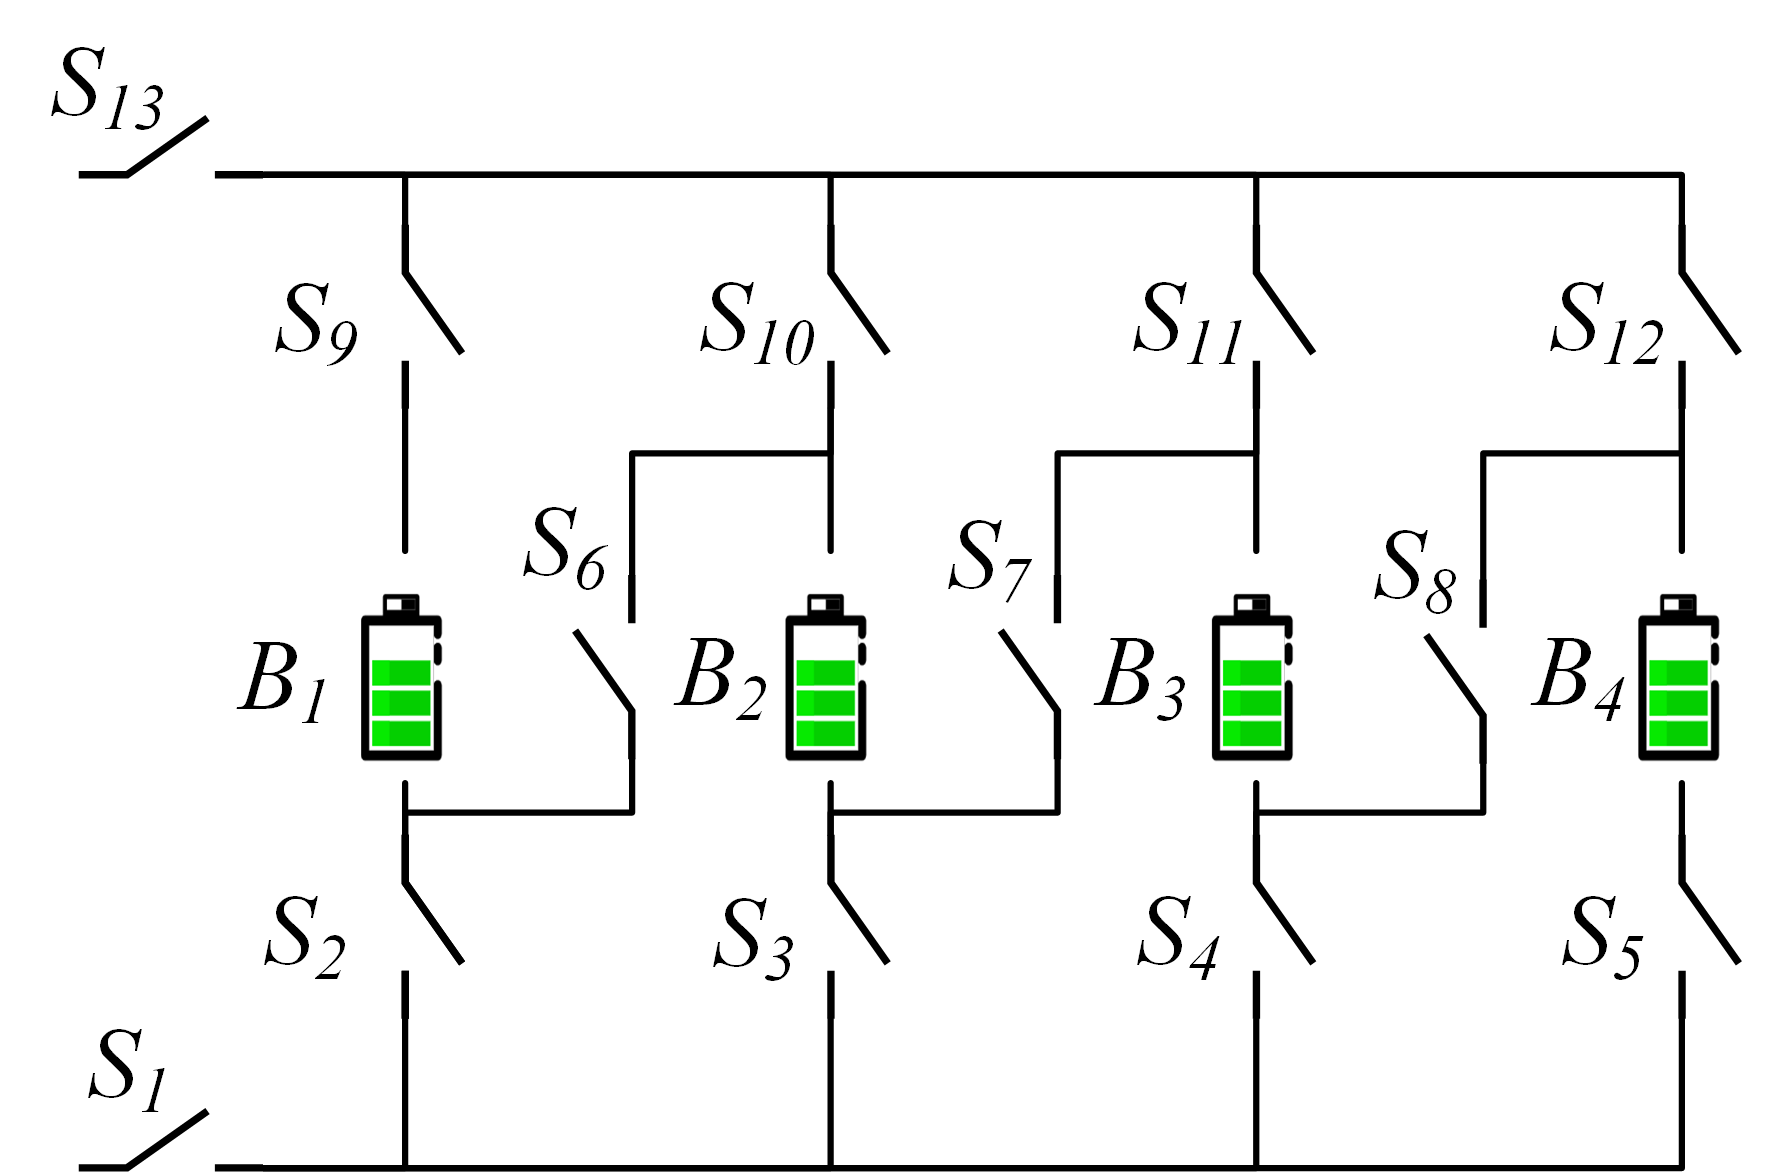
\includegraphics[width=\textwidth]{stru-V-origin.png}
%DIFDELCMD <         %%%
%DIFDELCMD < \caption{%
{%DIFAUXCMD
}
        %DIFAUXCMD
%DIFDELCMD < \label{fig:stru-Visairo}
%DIFDELCMD <     \end{subfigure}
%DIFDELCMD <     %%%
\DIFdelFL{\hspace{0.05\textwidth}
    }%DIFDELCMD < \begin{subfigure}[b]{0.45\textwidth}
%DIFDELCMD <         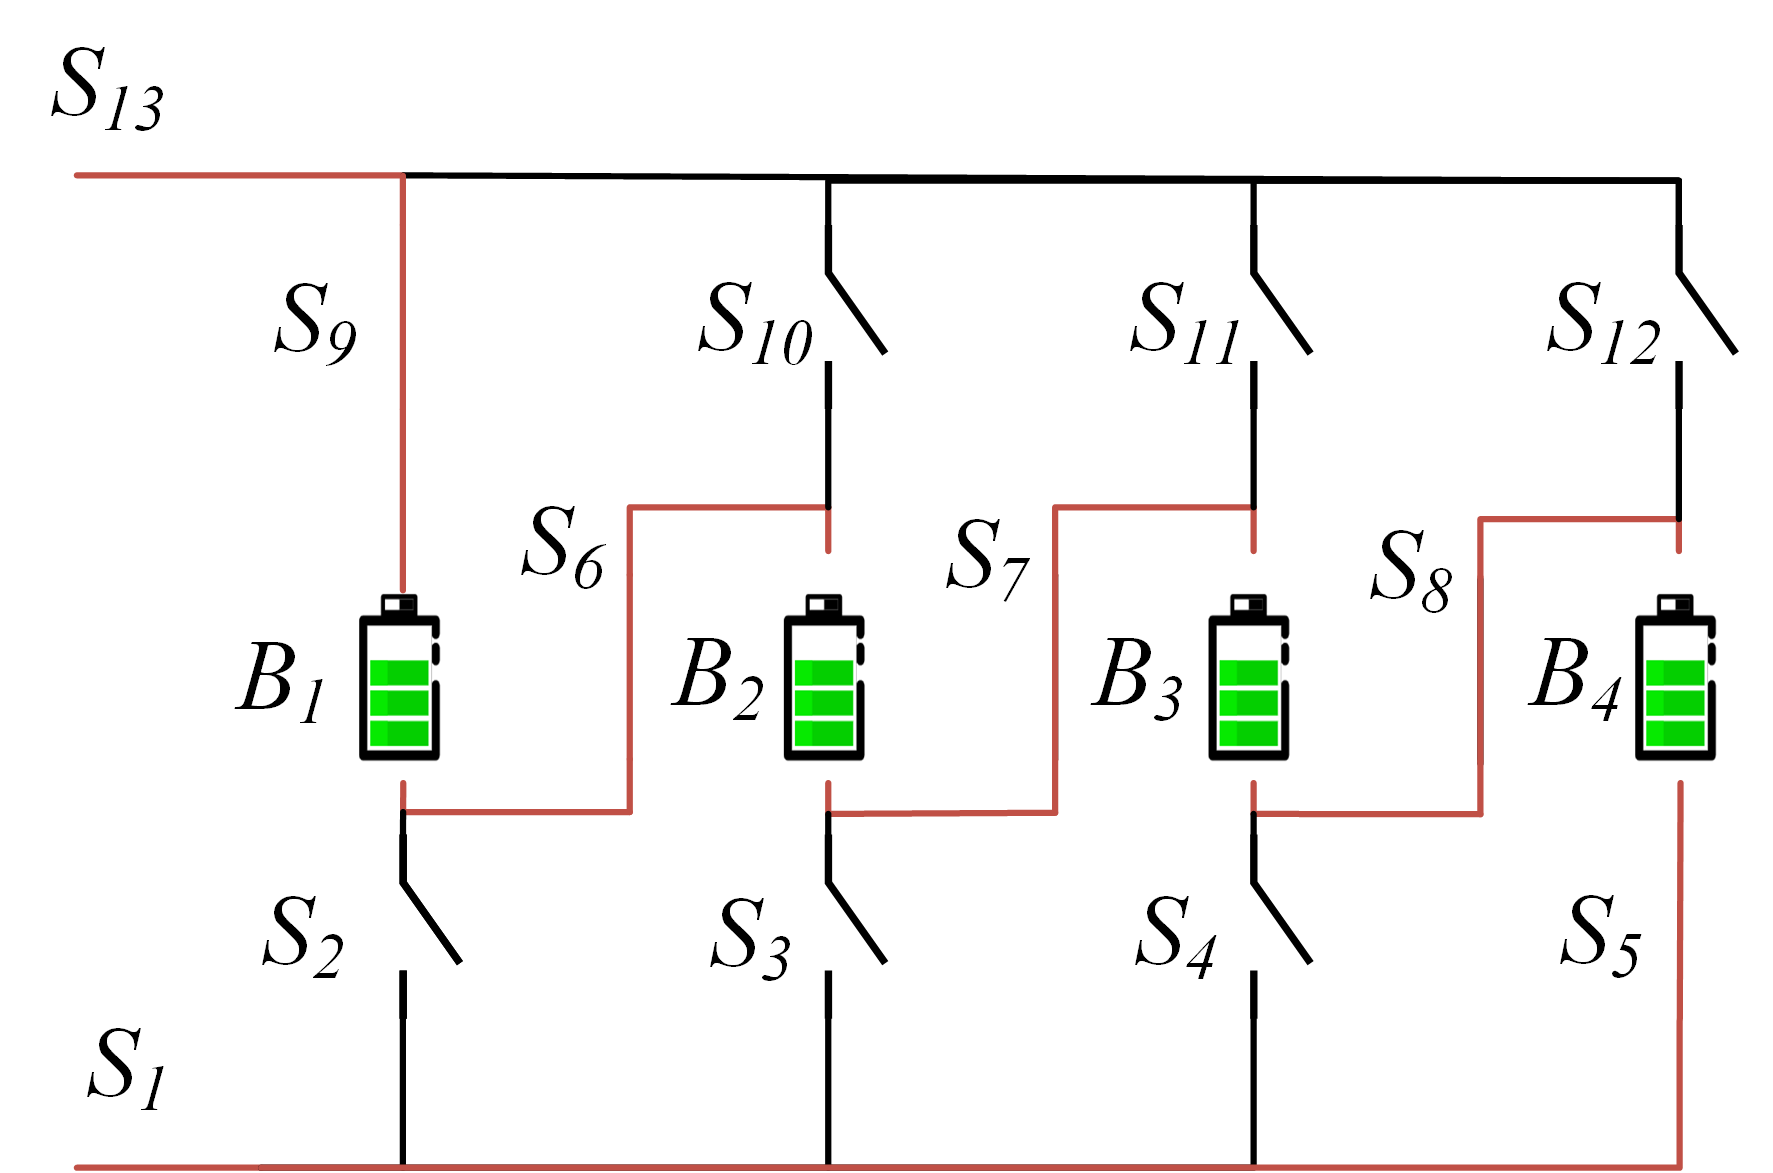
\includegraphics[width=\textwidth]{stru-V-serial.png}
%DIFDELCMD <         %%%
%DIFDELCMD < \caption{%
{%DIFAUXCMD
}
        %DIFAUXCMD
%DIFDELCMD < \label{fig:stru-Visairo-serial}
%DIFDELCMD <     \end{subfigure}
%DIFDELCMD <     \\
%DIFDELCMD <     \begin{subfigure}[b]{0.45\textwidth}
%DIFDELCMD <         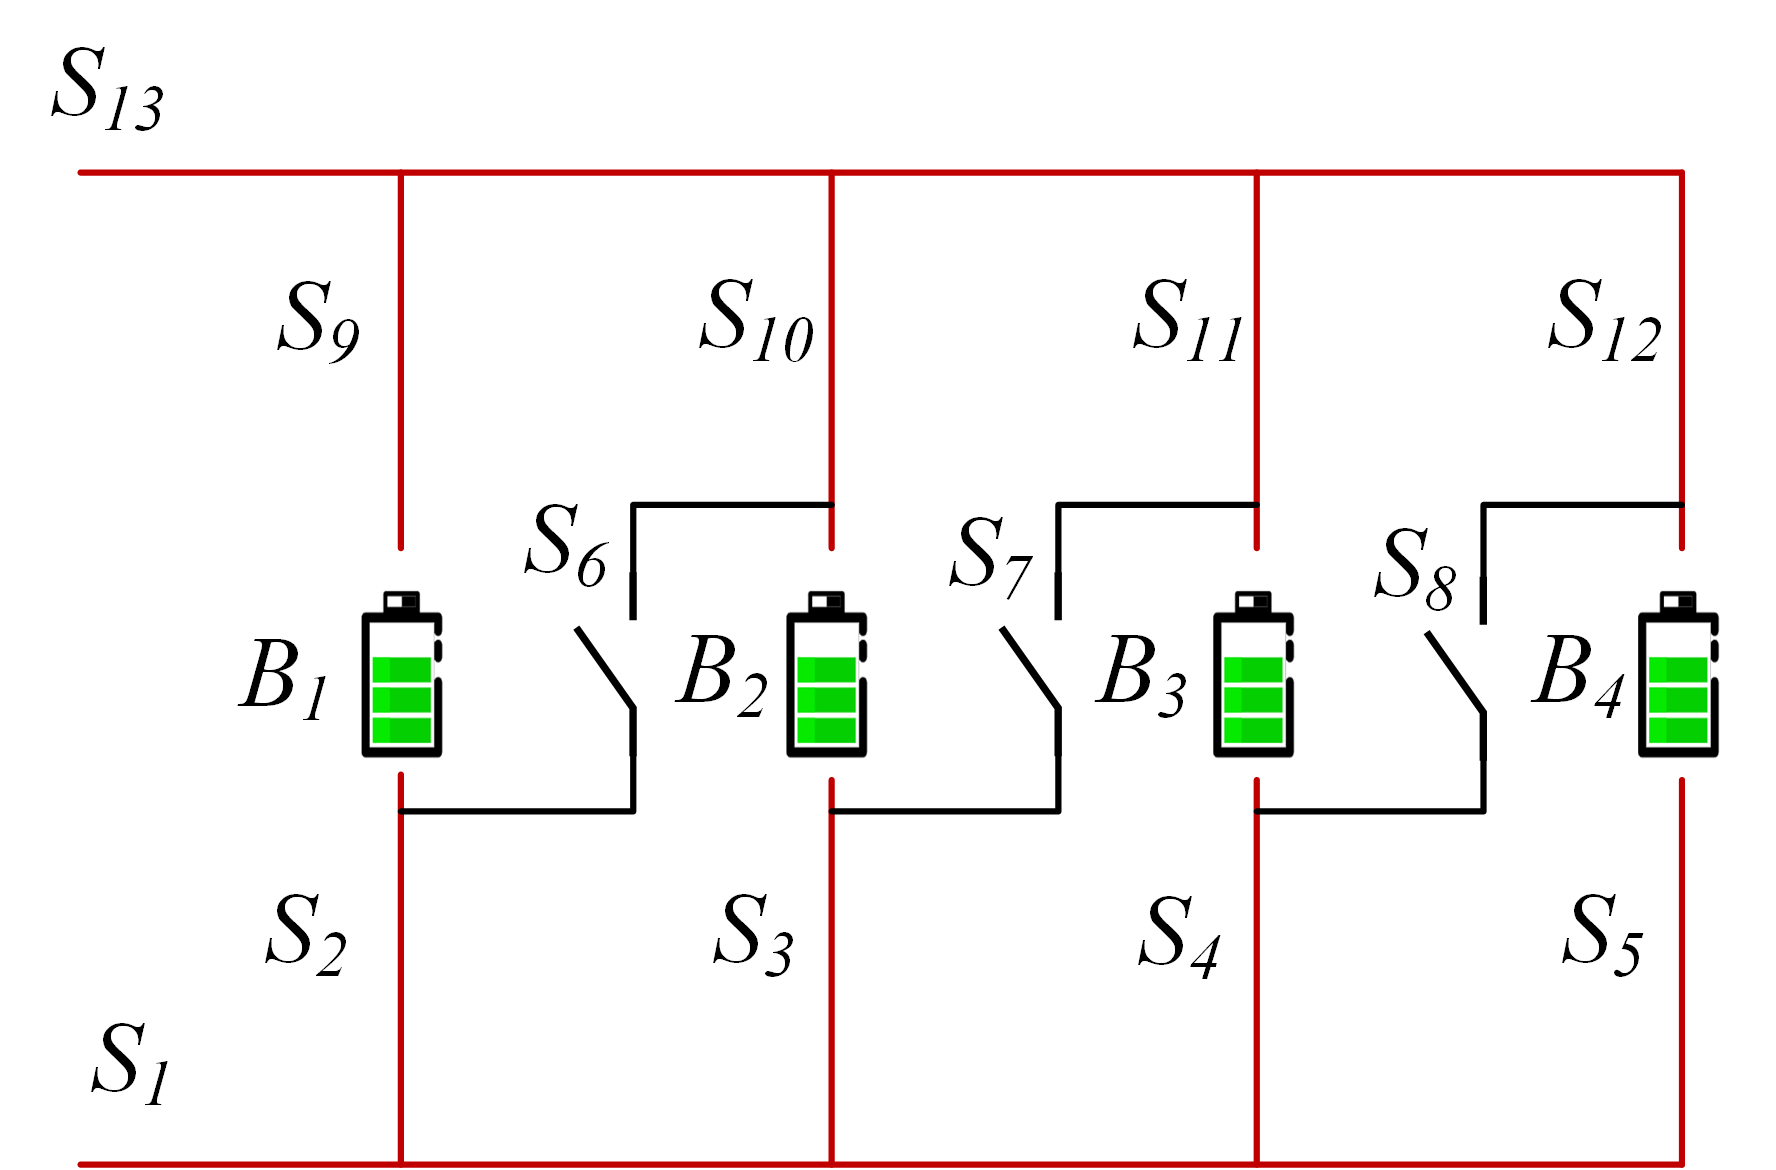
\includegraphics[width=\textwidth]{stru-V-parallel.png}
%DIFDELCMD <         %%%
%DIFDELCMD < \caption{%
{%DIFAUXCMD
}
        %DIFAUXCMD
%DIFDELCMD < \label{fig:stru-Visairo-parallel}
%DIFDELCMD <     \end{subfigure}
%DIFDELCMD <     %%%
\DIFdelFL{\hspace{0.05\textwidth}
    }%DIFDELCMD < \begin{subfigure}[b]{0.45\textwidth}
%DIFDELCMD <         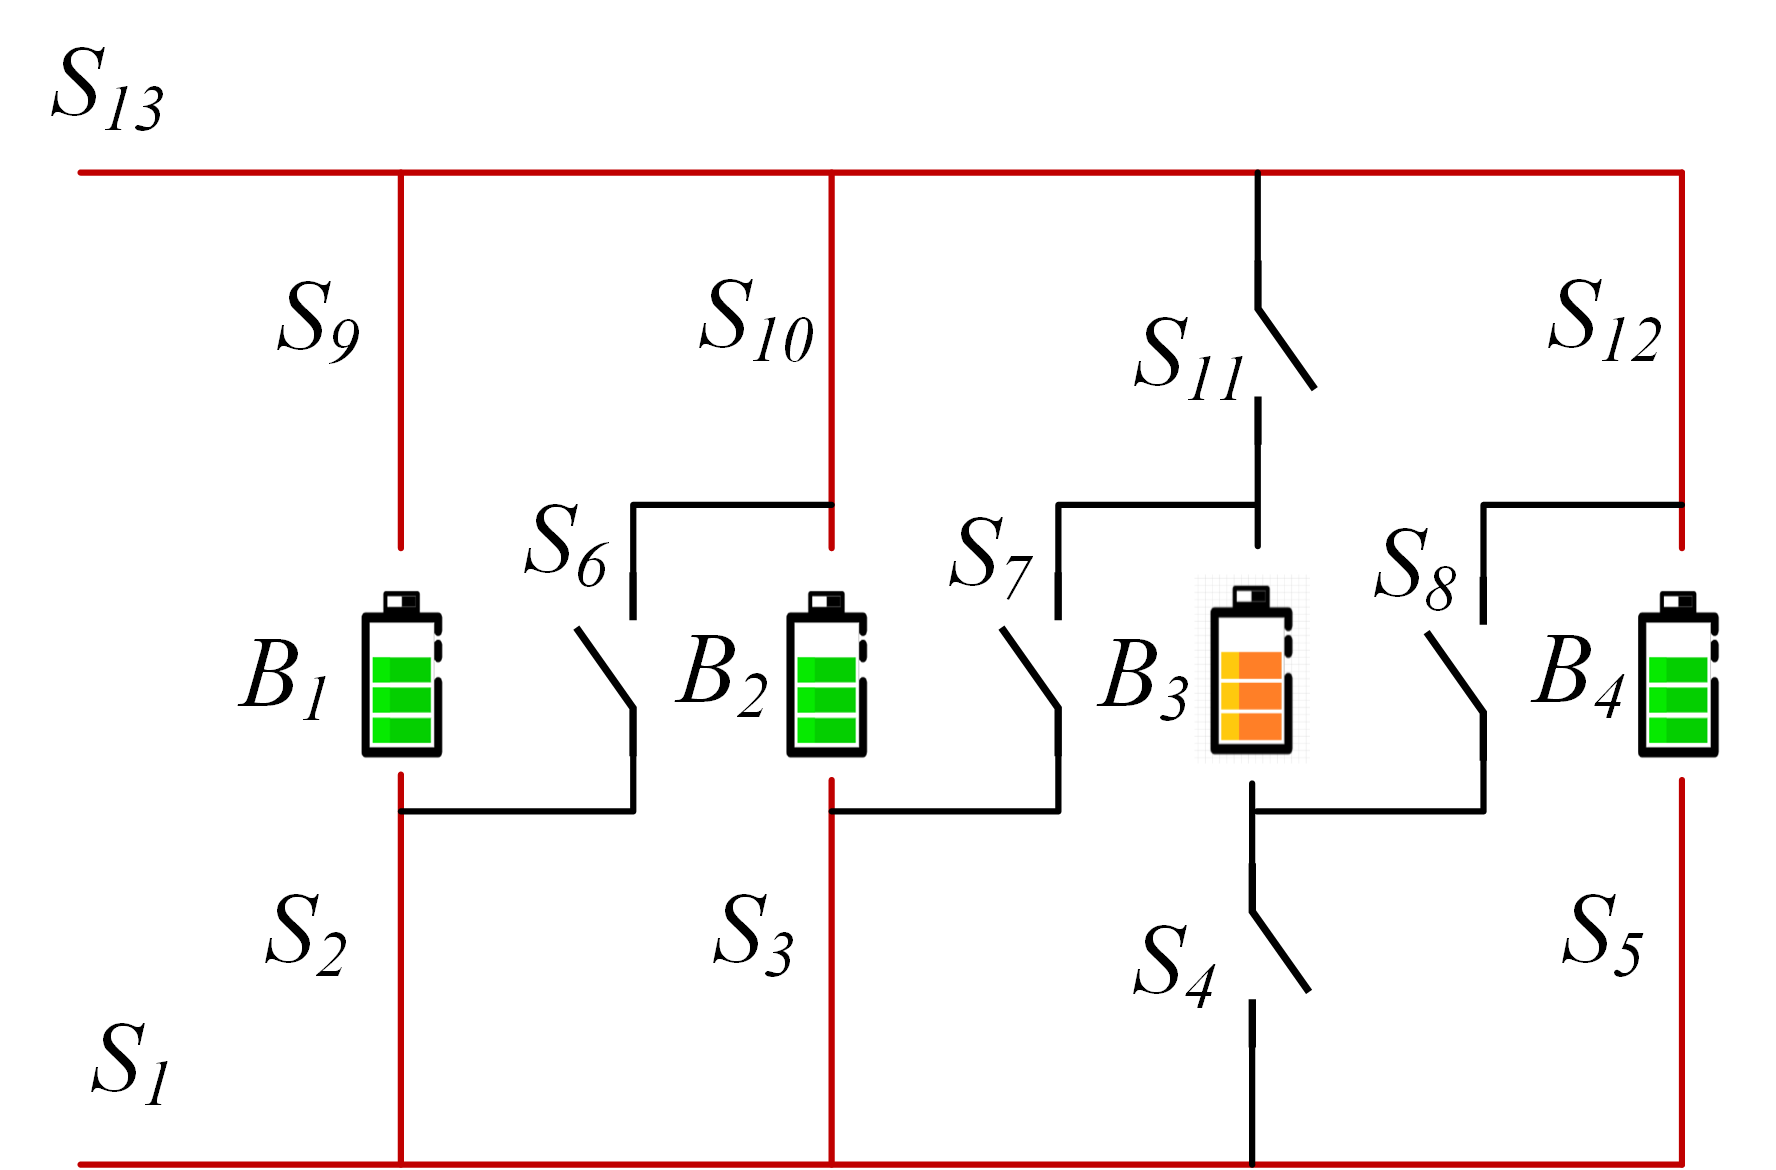
\includegraphics[width=\textwidth]{stru-V-isolate.png}
%DIFDELCMD <         %%%
%DIFDELCMD < \caption{%
{%DIFAUXCMD
}
        %DIFAUXCMD
%DIFDELCMD < \label{fig:stru-Visairo-isolate}
%DIFDELCMD <     \end{subfigure}
%DIFDELCMD <     %%%
%DIFDELCMD < \caption{%
{%DIFAUXCMD
\DIFdelFL{(a) The RBS structure proposed by Visairo\mbox{%DIFAUXCMD
\cite{visairoReconfigurableBatteryPack2008}}\hskip0pt%DIFAUXCMD
, with
        all batteries in (b) series connection, (c) parallel connection, and
        (d) battery $B_3$ isolated.
        }}
    %DIFAUXCMD
%DIFDELCMD < \label{fig:arch}
%DIFDELCMD < \end{figure}
%DIFDELCMD < 

%DIFDELCMD < %%%
%DIF < <*reviewer1-comment2>
\DIFdel{Recently, various types of RBSs with different }\DIFdelend \DIFaddbegin \DIFadd{The early research on RBSs mainly focused on the topological design of their structures, incorporating different levels of }\DIFaddend flexibility and reconfigurability \DIFdelbegin \DIFdel{have been designed }\DIFdelend to meet application requirements.
For example, Ci et al. \cite{ci2007novel} proposed an RBS structure that dynamically adjusts the battery discharge rate to fully exploit the available capacity of each battery. 
Jan \DIFdelbegin \DIFdel{'s \mbox{%DIFAUXCMD
\cite{9209774,engelhardt2021double} }\hskip0pt%DIFAUXCMD
structures  reconfigure structures }\DIFdelend \DIFaddbegin \DIFadd{et al. \mbox{%DIFAUXCMD
\cite{9209774,engelhardt2021double} }\hskip0pt%DIFAUXCMD
designed structures that reconfigure circuits }\DIFaddend with variant batteries in series to \DIFdelbegin \DIFdel{reach the (constantly changing ) }\DIFdelend \DIFaddbegin \DIFadd{accommodate the constantly changing }\DIFaddend voltage requirements during electric vehicle charging.
\DIFdelbegin \DIFdel{As shown in Fig. \ref{fig:stru-Visairo}, the }\DIFdelend \DIFaddbegin \DIFadd{A }\DIFaddend structure proposed by Visairo \DIFdelbegin \DIFdel{et al. \mbox{%DIFAUXCMD
\cite{visairoReconfigurableBatteryPack2008} }\hskip0pt%DIFAUXCMD
changes }\DIFdelend \DIFaddbegin \DIFadd{and Kumar \mbox{%DIFAUXCMD
\cite{visairoReconfigurableBatteryPack2008} }\hskip0pt%DIFAUXCMD
alters }\DIFaddend the system's output voltage based on the load conditions, thereby reducing \DIFdelbegin \DIFdel{the power loss of }\DIFdelend \DIFaddbegin \DIFadd{power loss in }\DIFaddend the voltage regulator during the power supply process and \DIFdelbegin \DIFdel{improving the efficiency of energy use. 
Also, to enhance the energy efficiencyof the system, Lawson et al. 
}\DIFdelend \DIFaddbegin \DIFadd{enhancing energy efficiency. 
Lawson }\DIFaddend \cite{lawsonSoftwareConfigurableBattery2012} and He et al. \cite{he2014reconfiguration} \DIFaddbegin \DIFadd{also focused on enhancing energy efficiency, and }\DIFaddend proposed simplified structures that have fewer switches than \DIFdelbegin \DIFdel{Visairo's design }\DIFdelend \DIFaddbegin \DIFadd{the design of Visairo and Kumar}\DIFaddend .
Kim et al. \cite{kim2009dynamic} improved the \DIFdelbegin \DIFdel{system's ability }\DIFdelend \DIFaddbegin \DIFadd{ability of an RBS structure }\DIFaddend to recover from battery failures by introducing multiple ports\DIFdelbegin \DIFdel{into the structure. 
}%DIFDELCMD < 

%DIFDELCMD < %%%
%DIF < <*reviewer1-comment8>
\DIFdel{The complex structure }\DIFdelend \DIFaddbegin \DIFadd{. 
%DIF > <*reviewer2-comment1>
These complex structures }\DIFaddend between batteries and switches \DIFdelbegin \DIFdel{gives RBSs flexibility but also creates challenges in the designand control of the system . 
Thus, several approaches to analyze the RBS structure and performance have been proposed to tackle these challenges. 
For instance, }\DIFdelend \DIFaddbegin \DIFadd{provide flexibility to RBSs but also pose challenges in hardware design. 
During the reconfiguration process, current deviation and fluctuation may occur. Specifically, when the system switches from series to parallel connection, a circulating current between parallel cells can be triggered due to a voltage imbalance \mbox{%DIFAUXCMD
\cite{hanAnalysisEstimationMaximum2020}}\hskip0pt%DIFAUXCMD
. Failure to fully consider this issue during the design of RBSs can result in damage to the batteries, switches, and wires. 
For example, Engelhardt et al. \mbox{%DIFAUXCMD
\cite{engelhardtDoubleStringBatterySystem2021} }\hskip0pt%DIFAUXCMD
applied an RBS to a fast-charging scenario with adaptive cell switching to balance cell states while adhering to voltage requests. However, the switching of batteries leads to intolerable current variations. 
To address this problem, }\DIFaddend Han et al. \cite{han2021analysis} derived an analytical expression for the maximum switch current during battery system reconfiguration\DIFdelbegin \DIFdel{for a specific RBS structure. This helps guide }\DIFdelend \DIFaddbegin \DIFadd{. This analytical expression aids in }\DIFaddend the selection of switches and supports \DIFdelbegin \DIFdel{the designof RBS hardware. 
}\DIFdelend \DIFaddbegin \DIFadd{general hardware design.
}


\DIFadd{Recently, increasing attention has been paid to the estimation and control of RBS system states, and several approaches have been proposed to optimize the performance of these systems. 
State estimation, which is an essential technology in traditional battery management systems, serves as the foundation for system control and holds great potential in the context of RBSs \mbox{%DIFAUXCMD
\cite{komsiyskaCriticalReviewIntelligent2021}}\hskip0pt%DIFAUXCMD
.
Couto et al. \mbox{%DIFAUXCMD
\cite{coutoPartitionbasedUnscentedKalman2018a} }\hskip0pt%DIFAUXCMD
introduced a partition-based unscented Kalman filter to estimate the state of a large-scale RBS, utilizing an enhanced reduced-order electrochemical model. 
Kersten et al. \mbox{%DIFAUXCMD
\cite{kerstenOnlineOnBoardBattery2020a} }\hskip0pt%DIFAUXCMD
utilized the balancing current of neighboring cells in parallel operation to determine the battery impedance, thereby obtaining information about the state of health and power capability of the RBS. 
Schmid et al. \mbox{%DIFAUXCMD
\cite{schmidActiveModelBasedFault2021a} }\hskip0pt%DIFAUXCMD
further leveraged the reconfigurable nature of the system to actively diagnose faults, employing an algorithm that changes the system structure to enhance the fault isolability. 
Another active research area is the development of effective control strategies for RBSs to achieve optimal performance, including improved stability \mbox{%DIFAUXCMD
\cite{kacetlDesignAnalysisModular2023b} }\hskip0pt%DIFAUXCMD
and efficiency \mbox{%DIFAUXCMD
\cite{yangAdaptiveControlFramework2022}}\hskip0pt%DIFAUXCMD
.
Han et al. \mbox{%DIFAUXCMD
\cite{hanNearFastestBatteryBalancing2019a} }\hskip0pt%DIFAUXCMD
proposed a near-fastest battery balancing algorithm to minimize the time required for battery charge equalization.
Liu et al. \mbox{%DIFAUXCMD
\cite{liuFlexiblePathPlanningbased2023a} }\hskip0pt%DIFAUXCMD
also proposed a scheme for maximizing capacity utilization based on a path planning algorithm, aiming to enhance the battery consistency within the system.
To break through the bottleneck of the potential short-circuit paths increasing exponentially with the RBS scale, }\DIFaddend Chen et al. \cite{chenSneakCircuitTheory2021} proposed a systematic approach based on sneak circuit theory\DIFdelbegin \DIFdel{to fundamentally avoid the short-circuit problem of RBSs: 
They thoroughly analyzed }\DIFdelend \DIFaddbegin \DIFadd{. 
They conducted a comprehensive analysis of }\DIFaddend all paths between the cathode and anode of each battery in the RBS\DIFdelbegin \DIFdel{and identified paths that only contain }\DIFdelend \DIFaddbegin \DIFadd{, identifying paths that consist only of }\DIFaddend switches as short-circuit paths for pre-checking before system reconfiguration. 
%DIF < </reviewer1-comment8>
\DIFaddbegin \DIFadd{Artificial intelligence has also appeared in RBS management \mbox{%DIFAUXCMD
\cite{liuLongLifetimeBattery2022a}}\hskip0pt%DIFAUXCMD
.
The effectiveness of the deep reinforcement learning method has been validated in real-world RBSs \mbox{%DIFAUXCMD
\cite{yangAdaptiveControlFramework2022}}\hskip0pt%DIFAUXCMD
.
%DIF > </reviewer2-comment1>
}\DIFaddend 


\DIFdelbegin \DIFdel{In spite of the maximum switch current mentioned above, the maximum }\DIFdelend \DIFaddbegin \DIFadd{The maximum }\DIFaddend allowable current (MAC), \DIFaddbegin \DIFadd{which is }\DIFaddend defined as the maximum \DIFdelbegin \DIFdel{allowed current under }\DIFdelend \DIFaddbegin \DIFadd{current allowed within }\DIFaddend the constraints of \DIFdelbegin \DIFdel{the }\DIFdelend \DIFaddbegin \DIFadd{a }\DIFaddend battery cell, is \DIFdelbegin \DIFdel{another critical }\DIFdelend \DIFaddbegin \DIFadd{a crucial }\DIFaddend indicator of RBSs that \DIFdelbegin \DIFdel{needs }\DIFdelend \DIFaddbegin \DIFadd{need }\DIFaddend to be evaluated during the design \DIFdelbegin \DIFdel{or }\DIFdelend \DIFaddbegin \DIFadd{and }\DIFaddend control of the system. 
The MAC \DIFdelbegin \DIFdel{helps the designers assess }\DIFdelend \DIFaddbegin \DIFadd{assists designers in assessing }\DIFaddend whether the RBS meets \DIFdelbegin \DIFdel{the }\DIFdelend output current requirements and contributes to the \DIFdelbegin \DIFdel{formulation }\DIFdelend \DIFaddbegin \DIFadd{development }\DIFaddend of appropriate and safe \DIFdelbegin \DIFdel{management }\DIFdelend strategies for the battery management system. 
\DIFdelbegin \DIFdel{Unfortunately}\DIFdelend %DIF > <*reviewer1-comment3>
\DIFaddbegin \DIFadd{However}\DIFaddend , few studies have \DIFdelbegin \DIFdel{analyzed the RBS structure to determine the RBS MAC. 
An intuitive and straightforward method is to enumerate all possible switch states and calculate the output current of }\DIFdelend \DIFaddbegin \DIFadd{directly determined the MACs of RBSs, primarily due to }\DIFaddend the \DIFdelbegin \DIFdel{system under each reconfigurated structure}\DIFdelend \DIFaddbegin \DIFadd{complexity arising from reconfiguration. 
In the field of computer science, there is a similar problem with scheduling tasks on dynamically reconfigurable hardware with limited resources and task interdependencies. This problem is analogous to the determination of the MAC and a corresponding solution has been proposed \mbox{%DIFAUXCMD
\cite{mollajafariEfficientLightweightAlgorithm2023,heReconfigurationassistedChargingLargescale2014}}\hskip0pt%DIFAUXCMD
. 
However, dealing with the structural characteristics and circuit equations of RBSs is challenging for this method. 
%DIF > </reviewer1-comment3>
From the perspective of RBS structure analysis, the MAC problem can be transformed into a problem of finding the maximum output current among all possible reconfigurations of the RBS}\DIFaddend . 
However, this \DIFdelbegin \DIFdel{method is inefficient and time-consuming, especially for RBSs with a large number of switches.
%DIF < </reviewer1-comment2>
}\DIFdelend \DIFaddbegin \DIFadd{may be an NP-hard problem \mbox{%DIFAUXCMD
\cite{pinterReviewControlAlgorithms2021a}}\hskip0pt%DIFAUXCMD
. 
Common methods such as brute-force algorithms, simulated annealing (SA) algorithms, and genetic algorithms (GA) have the drawbacks of inefficiency, excessive time consumption, and an inability to guarantee the globally optimal solution.
}\DIFaddend 


To solve this issue, this paper proposes an efficient method to evaluate the \DIFdelbegin \DIFdel{MAC }\DIFdelend \DIFaddbegin \DIFadd{MACs }\DIFaddend of RBSs. 
In this method, a greedy algorithm is designed to efficiently search the possible circuit \DIFdelbegin \DIFdel{topology of RBSswith MAC}\DIFdelend \DIFaddbegin \DIFadd{topologies of RBSs}\DIFaddend .
This algorithm transforms the \DIFdelbegin \DIFdel{enumeration of switch states in the brute-force algorithm into the combination of the batteries' shortest paths .
An improved direct graph model that considers the }\DIFdelend \DIFaddbegin \DIFadd{inefficient search for reconfigurations into a proactive combining of the shortest paths of the batteries.
Furthermore, an improved directed graph model is introduced to analyze the current of the RBS, taking into account factors such as the }\DIFaddend voltage, \DIFdelbegin \DIFdel{the }\DIFdelend internal resistance, \DIFdelbegin \DIFdel{the }\DIFdelend MAC of the battery, and \DIFdelbegin \DIFdel{the external loadis also introduced to analyze the current of the RBS. 
%DIF < <*reviewer1-comment3>
}\DIFdelend \DIFaddbegin \DIFadd{external load. 
}\DIFaddend The main contributions of this \DIFdelbegin \DIFdel{paper }\DIFdelend \DIFaddbegin \DIFadd{study }\DIFaddend can be summarized as follows:
\begin{itemize}
  \item An efficient method is proposed to determine the \DIFdelbegin \DIFdel{MAC }\DIFdelend \DIFaddbegin \DIFadd{MACs }\DIFaddend of RBSs with arbitrary structures, including scenarios with isolated batteries.
  \item A greedy algorithm is applied to solve the MAC problem, the computational complexity of which is greatly reduced compared with the brute-force algorithm.
  \item An improved directed graph model is introduced to provide a specific method for calculating the MAC of a given structure.
\end{itemize}
%DIF < </reviewer1-comment3>


The remainder of this paper is organized as follows: 
Section II presents the framework and details of the proposed directed graph model and \DIFaddbegin \DIFadd{the }\DIFaddend greedy algorithm. 
Section III \DIFdelbegin \DIFdel{discusses a case study that uses }\DIFdelend \DIFaddbegin \DIFadd{applies }\DIFaddend the proposed method to determine the MACs of two published \DIFdelbegin \DIFdel{four-battery RBSs and }\DIFdelend \DIFaddbegin \DIFadd{RBS structures and a new }\DIFaddend one with a more complex structure. 
The calculation results, the \DIFdelbegin \DIFdel{algorithm's computational complexity }\DIFdelend \DIFaddbegin \DIFadd{computational complexity of the algorithm}\DIFaddend , and scenarios such as battery random isolation are also discussed. 
Finally, the concluding remarks are presented in Section IV.

\section{Methodology}

The central principle of \DIFdelbegin \DIFdel{this }\DIFdelend \DIFaddbegin \DIFadd{the proposed }\DIFaddend method is to connect the batteries in an RBS in parallel to the \DIFdelbegin \DIFdel{extent possible }\DIFdelend \DIFaddbegin \DIFadd{maximum possible extent}\DIFaddend , thereby maximizing the output current\DIFdelbegin \DIFdel{of the RBS}\DIFdelend .
To achieve this universally and automatically, the overall process is divided into the four steps shown in Fig. \ref{fig:main}.
First, a directed graph model is established for \DIFaddbegin \DIFadd{the }\DIFaddend subsequent computations. The model not only contains the connected relationships between batteries and switches but also retains the performance parameters of the batteries.
Subsequently, based on the equivalent circuit, the MAC problem is transformed into specific objective functions and constraints.
The shortest paths (SPs, where additional batteries and switches on the path are penalized \DIFdelbegin \DIFdel{as distance) for }\DIFdelend \DIFaddbegin \DIFadd{for distance) of }\DIFaddend the batteries are then obtained \DIFdelbegin \DIFdel{by }\DIFdelend using the Dijkstra algorithm to connect the batteries in the RBS in parallel.
Finally, a greedy algorithm is used to organize the switches, allowing the batteries to connect via their SPs while satisfying the constraints, resulting in the MAC of the RBS.

\begin{figure}[htbp]
    \centering
    \begin{subfigure}[b]{0.8\textwidth}
        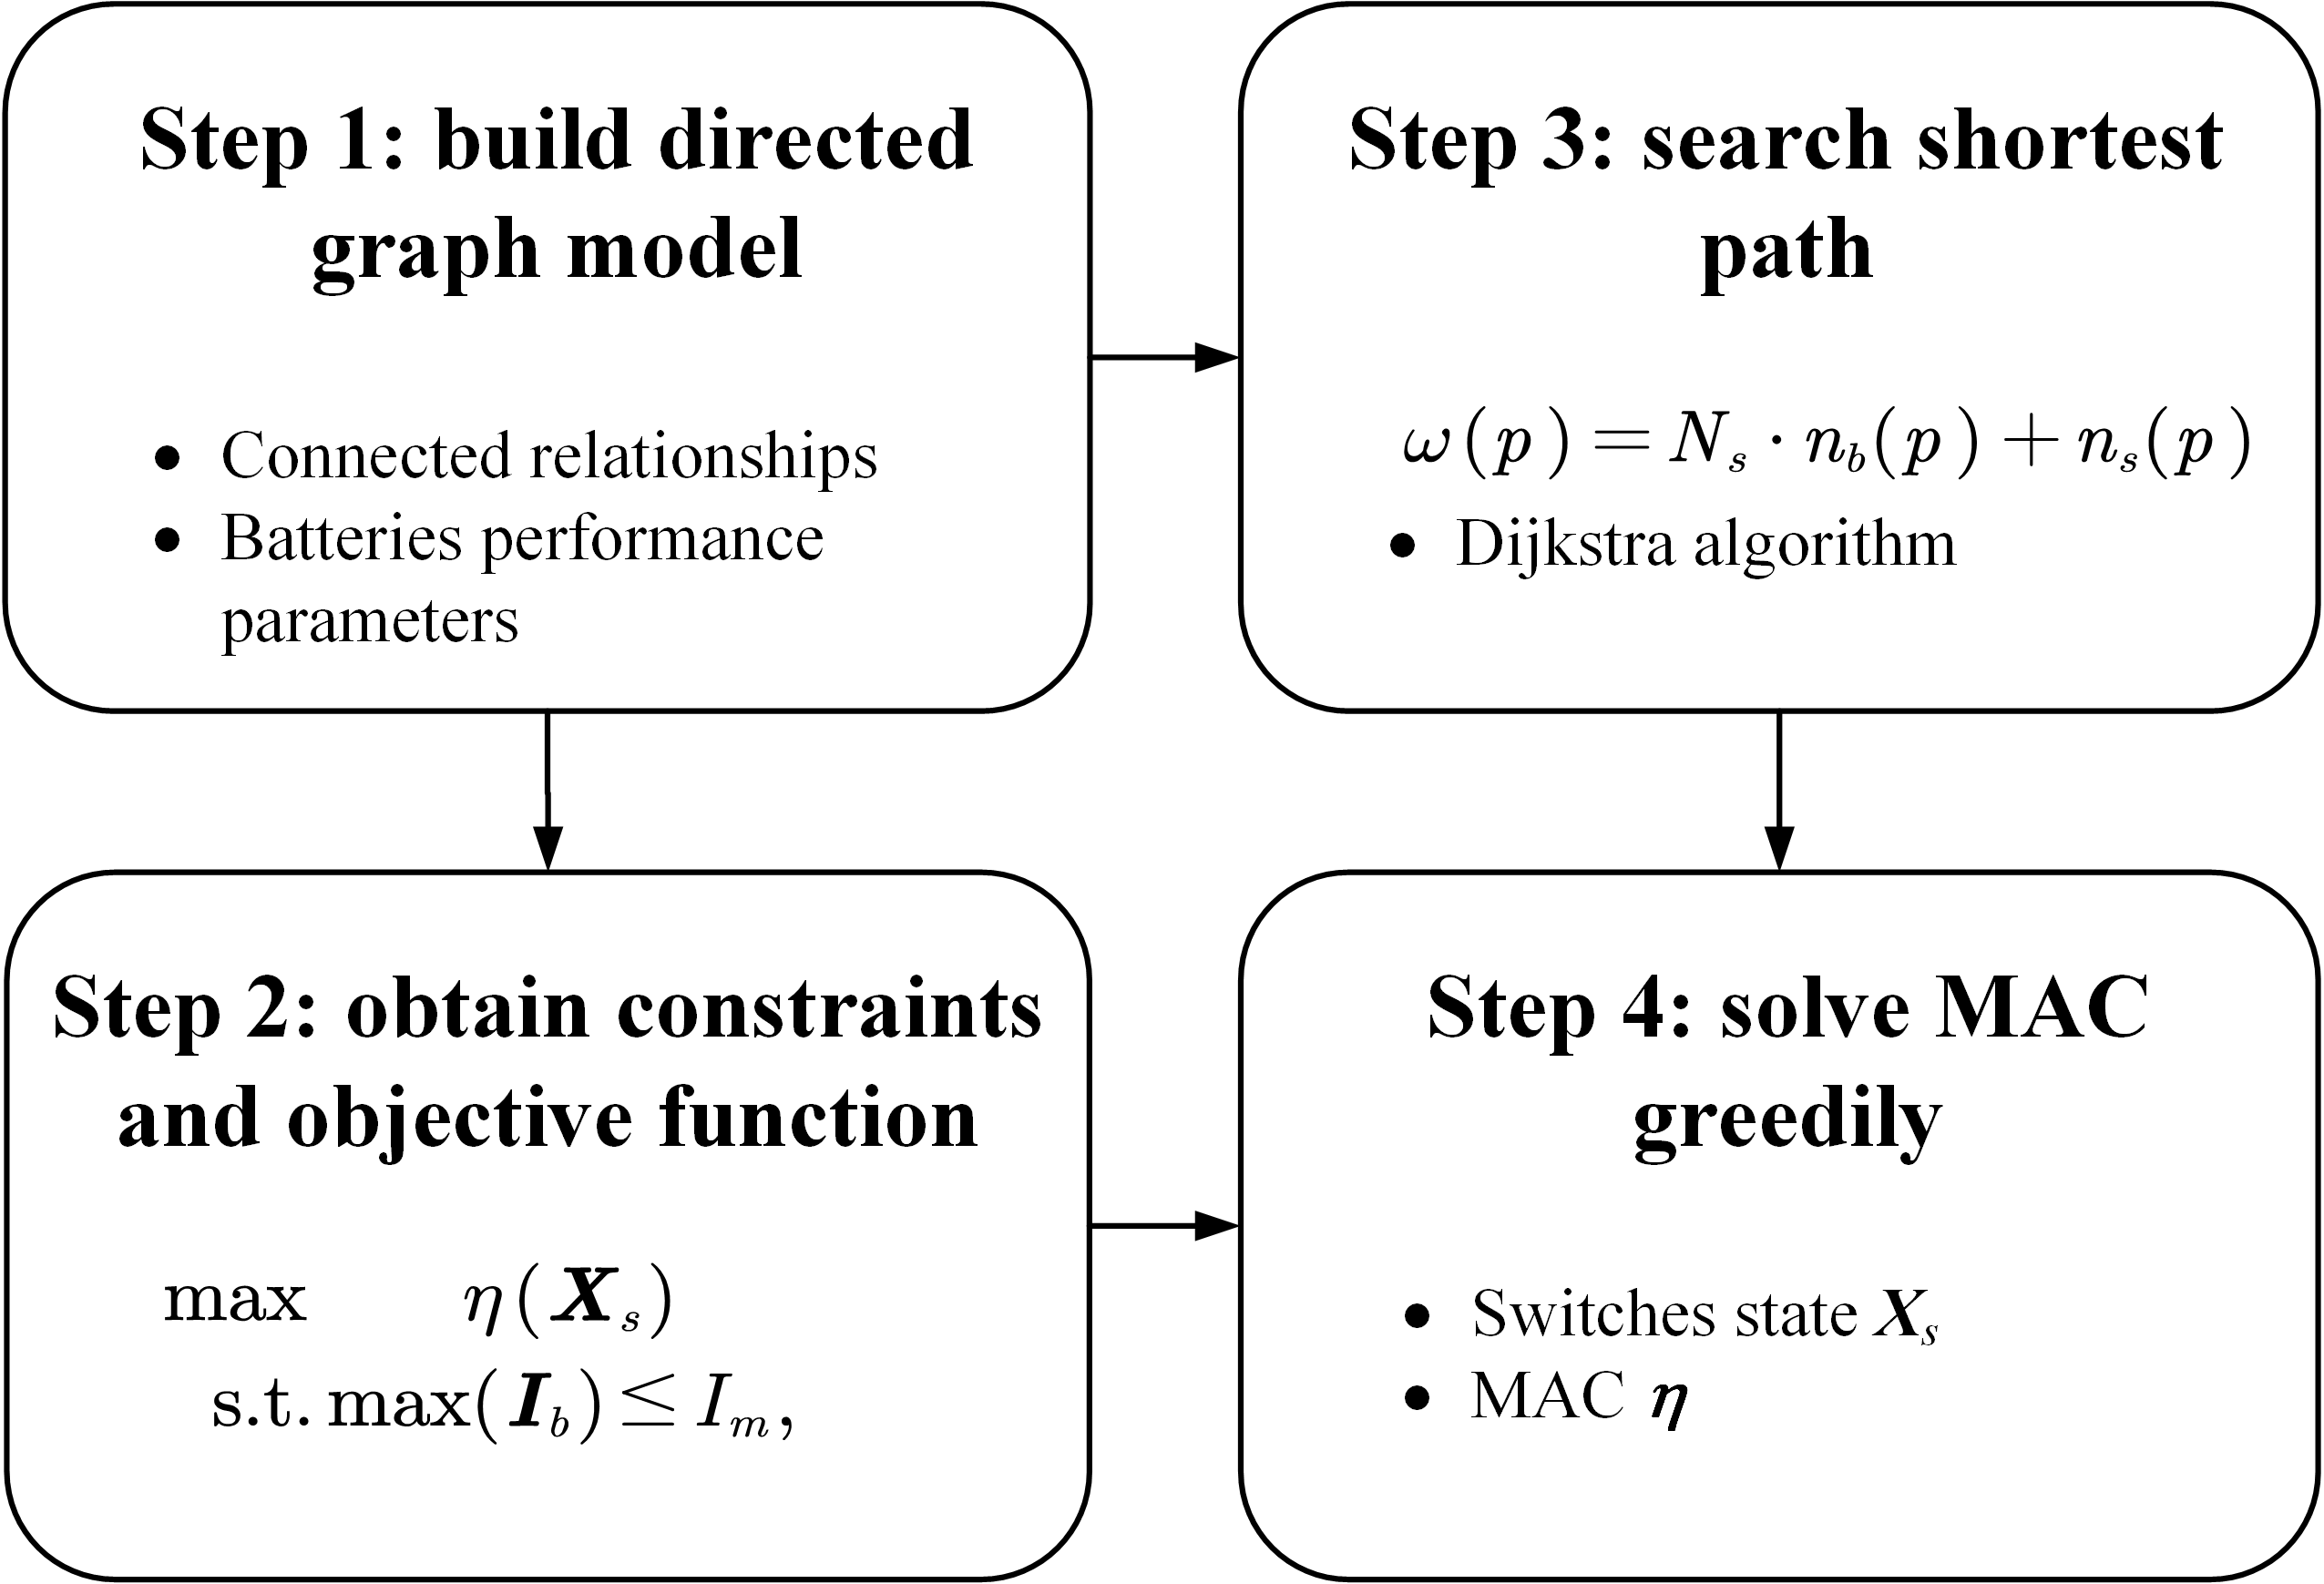
\includegraphics[width=\textwidth]{main.png}
    \end{subfigure}
    \caption{ 
        \DIFdelbeginFL \DIFdelFL{Diagram }\DIFdelendFL \DIFaddbeginFL \DIFaddFL{A diagram }\DIFaddendFL of \DIFdelbeginFL \DIFdelFL{this }\DIFdelendFL \DIFaddbeginFL \DIFaddFL{the proposed }\DIFaddendFL method, which contains four main steps.
    }
    \label{fig:main}
\end{figure}

\subsection{Directed graph model}

\begin{figure}[htbp]
    \centering
    \begin{subfigure}[b]{0.31\textwidth}
        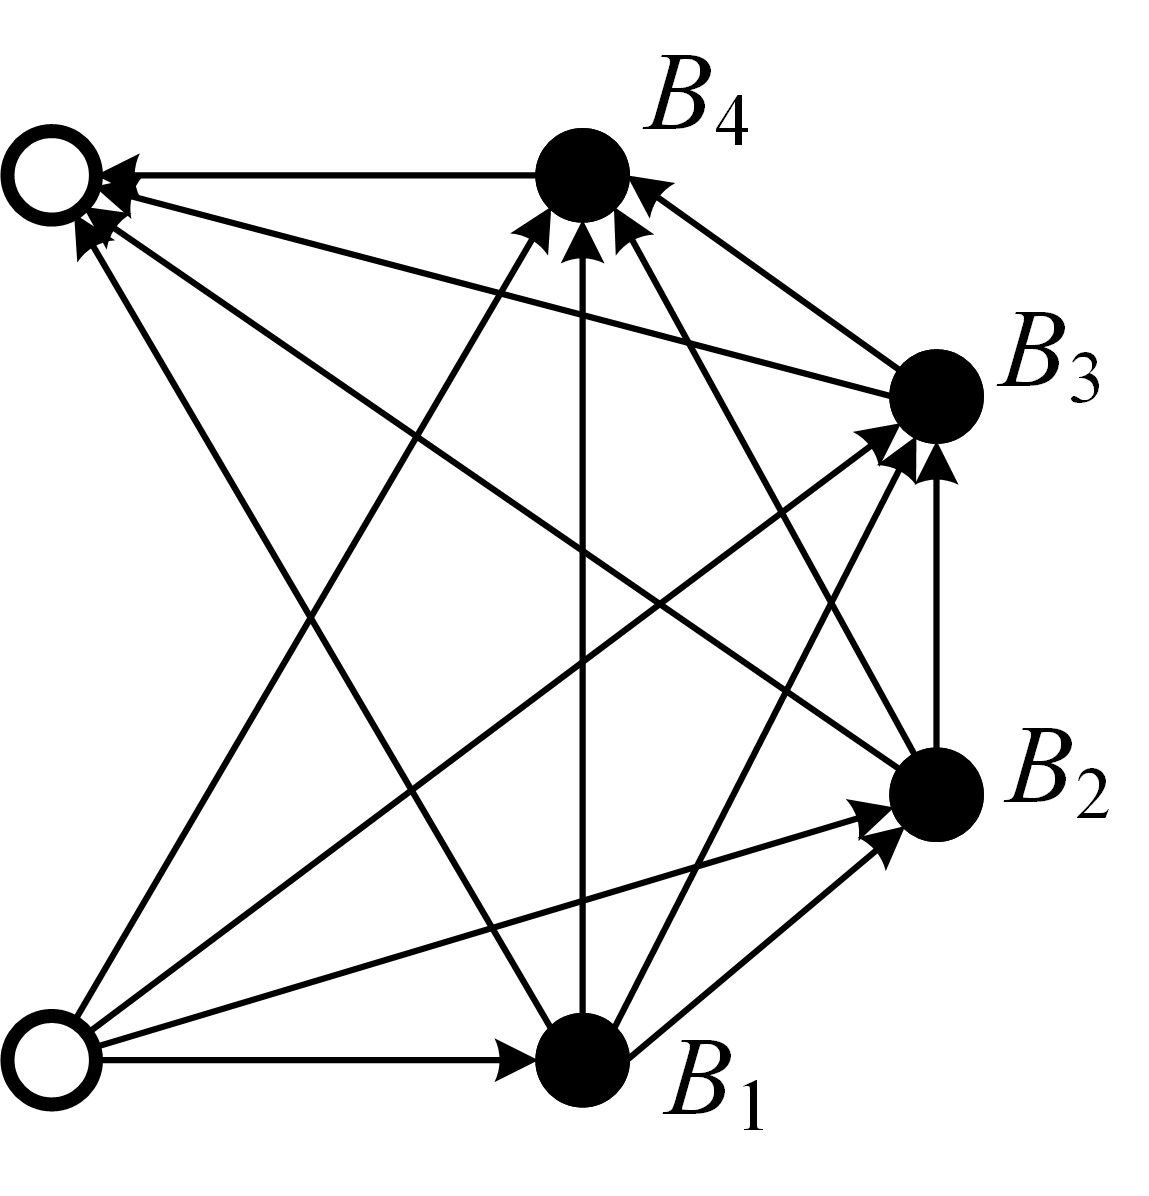
\includegraphics[width=\textwidth]{direct-graph-he.png}
        \caption{}
        \label{fig:direct-graph-he}
    \end{subfigure}
    \hspace{0.02\textwidth}
    \begin{subfigure}[b]{0.23\textwidth}
        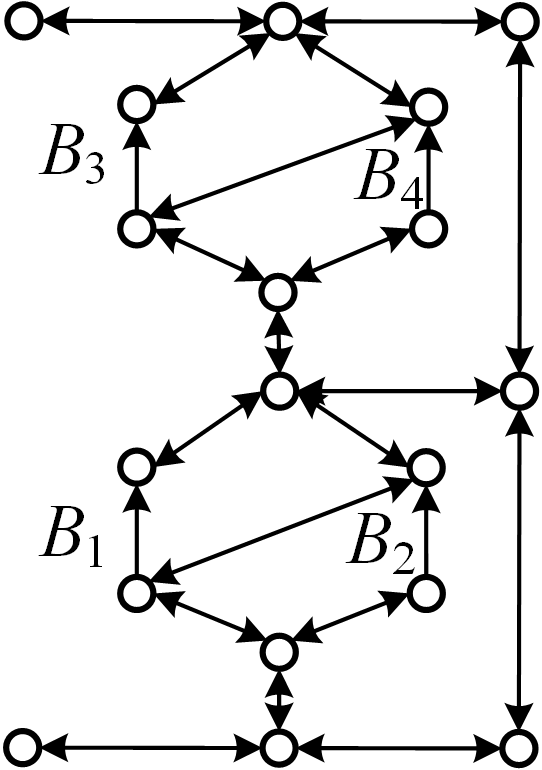
\includegraphics[width=\textwidth]{direct-graph-xu.png}
        \caption{}
        \label{fig:direct-graph-xu}
    \end{subfigure}
    \hspace{0.02\textwidth}
    \begin{subfigure}[b]{0.24\textwidth}
        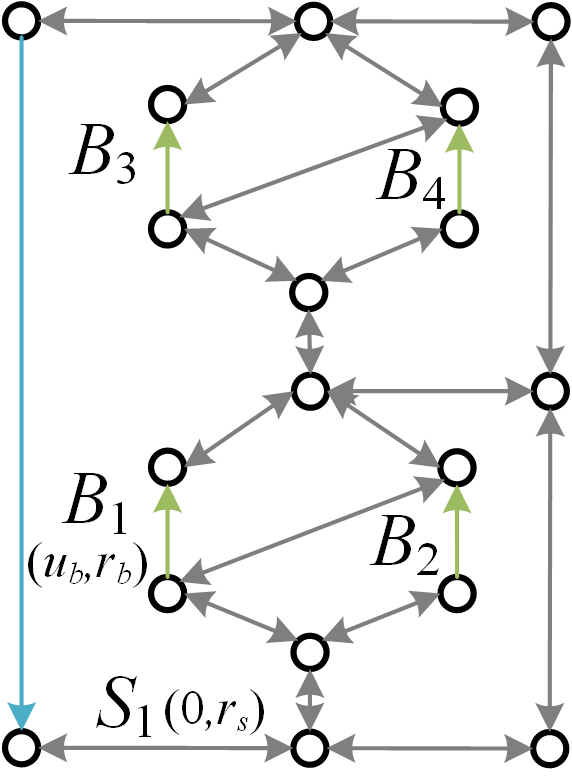
\includegraphics[width=\textwidth]{direct-graph-my.png}
        \caption{}
        \label{fig:direct-graph-my}
    \end{subfigure}
    \\
    \begin{subfigure}[b]{0.8\textwidth}
        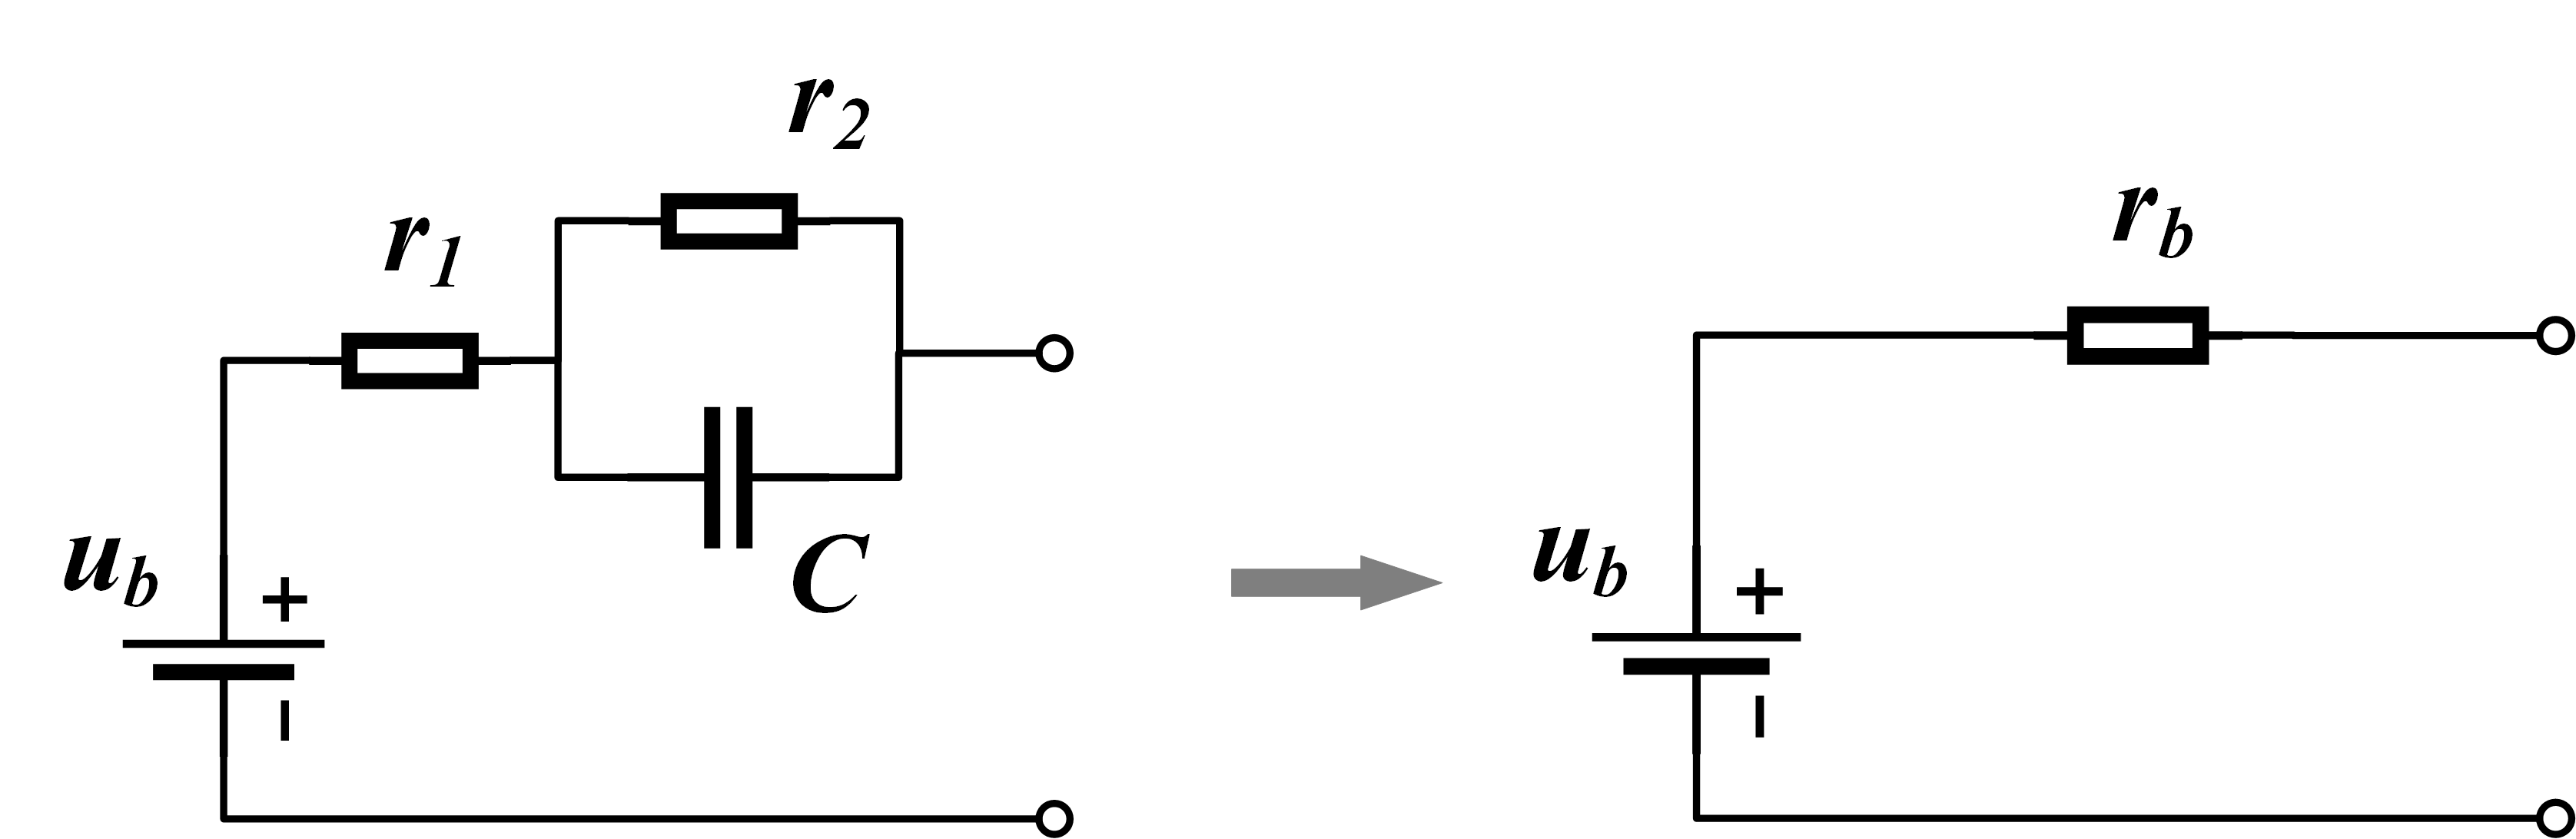
\includegraphics[width=\textwidth]{battery_simple.png}
        \caption{}
        \label{fig:battery_simple}
    \end{subfigure}
    \caption{ 
        \DIFdelbeginFL \DIFdelFL{Directed }\DIFdelendFL \DIFaddbeginFL \DIFaddFL{The directed }\DIFaddendFL graph models used in (a) \DIFdelbeginFL \DIFdelFL{He's }\DIFdelendFL \DIFaddbeginFL \DIFaddFL{the }\DIFaddendFL work \DIFaddbeginFL \DIFaddFL{of He et al. }\DIFaddendFL \cite{heExploringAdaptiveReconfiguration2013}, (b) our previous work, and (c) the improved model in this paper.
        (d) The equivalent circuit of a battery in this method.
    }
\end{figure}

He et al. \cite{heExploringAdaptiveReconfiguration2013} proposed an abstracted directed graph model for an RBS, where the nodes represent the batteries, the edges represent the configuration flexibility, and the weight of each vertex corresponds to the battery voltage (Fig. \ref{fig:direct-graph-he}). 
The model captures all potential system configurations and offers a direct metric for configuration flexibility, but it does not specify the physical implementation of the connectivity between batteries, meaning that one graph might correspond to multiple RBS structures.
We previously proposed a directed graph model that differs \DIFdelbegin \DIFdel{completely from He }\DIFdelend \DIFaddbegin \DIFadd{significantly from He et al.}\DIFaddend 's model by using nodes to represent the connections between batteries and switches and directed edges to represent batteries and switches (Fig. \ref{fig:direct-graph-xu}), allowing for a one-to-one correspondence between \DIFdelbegin \DIFdel{the }\DIFdelend \DIFaddbegin \DIFadd{an }\DIFaddend RBS structure and \DIFdelbegin \DIFdel{the }\DIFdelend \DIFaddbegin \DIFadd{its }\DIFaddend directed graph model. 
This model accurately and comprehensively represents the RBS topological structure but cannot be used for quantitative MAC calculations because it does not consider the voltage, internal resistance, \DIFdelbegin \DIFdel{and }\DIFdelend \DIFaddbegin \DIFadd{or }\DIFaddend MAC of the battery. 
To address this issue, we improve our previous model by adding electromotive force and resistance attributes on the edges based on \DIFdelbegin \DIFdel{its }\DIFdelend \DIFaddbegin \DIFadd{the corresponding }\DIFaddend equivalent circuits.
The model also considers the external load as an equivalent resistance and integrates it into the analysis, making it a complete circuit model for later circuit \DIFdelbegin \DIFdel{analyses}\DIFdelend \DIFaddbegin \DIFadd{analysis}\DIFaddend .
Fig. \ref{fig:direct-graph-my} shows the improved directed graph model used in this paper.
The following provides a detailed explanation of the method \DIFaddbegin \DIFadd{used }\DIFaddend for equating components in RBSs and constructing the directed graph model.


To use circuit analysis methods to solve the MAC of the RBS, the components in the RBS are equated to ideal circuit elements.
For instance, as shown in Fig. \ref{fig:battery_simple}, the battery in the RBS is represented as a black-box circuit consisting of two resistors $r_1$ and $r_2$ and a capacitor $C$, \DIFaddbegin \DIFadd{in what is }\DIFaddend known as the Thevenin model \cite{hongwenheStateofChargeEstimationLithiumIon2011,mousavig.VariousBatteryModels2014}.
With an emphasis on the stable output of the RBS, the capacitor in the Thevenin model can be considered as an open circuit without affecting the steady-state current.
Therefore, battery $B_i$ in the RBS can be simplified as a series connection between a constant voltage source $u_{i}$ and a resistor $r_{i}$.
Furthermore, the state of \DIFaddbegin \DIFadd{the }\DIFaddend switch $S_j$ in the RBS is represented by a binary variable $x_j$, where 0 is ON and 1 is OFF.
When the switch is closed, the circuit can be regarded as a resistor with a very small resistance $r_{j}$.
Finally, the external load is considered as a resistor with resistance $R_o$.


For a given RBS structure, its directed graph model $G(V,E)$ is constructed as follows:
\begin{enumerate}
    \item Nodes:
        The nodes in the directed graph correspond to the connection points of components in the actual RBS. 
        Assuming there are a total of $N$ nodes in the RBS, for the sake of convenience, the anode of the RBS is denoted as $v_1$ and the cathode as $v_N$.
    \item Edges:
        The edges in the directed graph correspond to the batteries, switches, and external electrical loads in the actual RBS.
        Therefore, there are three types of directed edges. 
        For battery $B_i$, its directed edge $e_i$ is drawn from the cathode to the anode because the battery in operation only allows current to flow in one direction.
        For switch $S_j$, since it is allowed to work under bidirectional currents, it is represented by a pair of directed edges with two-way directions. 
        \DIFdelbegin \DIFdel{Regarding the external electronic }\DIFdelend \DIFaddbegin \DIFadd{For the external electrical }\DIFaddend load, because it is connected to the anode and cathode of the RBS, a directed edge from $v_N$ to $v_1$ \DIFdelbegin \DIFdel{represents }\DIFdelend \DIFaddbegin \DIFadd{is used to represent }\DIFaddend it. 
        In conclusion, for a given RBS structure with $N_b$ batteries and $N_s$ switches, the number of directed edges is $N_b+2N_s+1$, where 1 \DIFdelbegin \DIFdel{refers to }\DIFdelend \DIFaddbegin \DIFadd{represents }\DIFaddend the external electrical load.
    \item Attributes of edges:
        Each edge is assigned two attributes, \DIFaddbegin \DIFadd{a }\DIFaddend voltage difference and \DIFaddbegin \DIFadd{a }\DIFaddend resistance, based on the equivalent method mentioned above.
        The values for battery $B_i$, switch $S_j$, and \DIFaddbegin \DIFadd{the }\DIFaddend external loads correspond to $(u_i, r_i)$, $(0, r_j)$, and $(0, R_o)$, respectively.
\end{enumerate}

\subsection{Constraints and objective function}

For a given RBS, determining \DIFdelbegin \DIFdel{its }\DIFdelend \DIFaddbegin \DIFadd{the }\DIFaddend MAC involves maximizing the RBS output current while ensuring that all battery currents do not exceed the batteries' MAC. 
This subsection establishes the constraints and objective function \DIFaddbegin \DIFadd{used }\DIFaddend to determine the \DIFdelbegin \DIFdel{RBS's }\DIFdelend MAC through circuit analysis based on the directed graph model provided in the previous section.


First, the topology in the directed graph model is represented in \DIFdelbegin \DIFdel{matrix form }\DIFdelend \DIFaddbegin \DIFadd{the form of a matrix }\DIFaddend $\bm{A}$, \DIFaddbegin \DIFadd{which is }\DIFaddend known as the incidence matrix and \DIFaddbegin \DIFadd{is }\DIFaddend defined as follows:
\begin{align}\label{eq:A}
    a_{kl}=
    \begin{cases}
        1,  & \text{edge $l$ leaves node $k$},\\
        -1, & \text{edge $l$ enters node $k$},\\
        0,  & \text{otherwise}.
    \end{cases}
\end{align}
For a directed graph consisting of $N$ nodes and $N_b+2N_s+1$ directed edges, \DIFdelbegin \DIFdel{its }\DIFdelend \DIFaddbegin \DIFadd{the }\DIFaddend incidence matrix $\bm{A}$ is an $N\times(N_b+2N_s+1)$ matrix. 
In this matrix, the rows and columns represent the nodes and edges of the directed graph, respectively.
By distinguishing the components in the RBS corresponding to each column, $\bm{A}$ can be rewritten as
\begin{equation}\label{eq:A_bso}
    \bm{A} =
    \begin{bmatrix}
        \bm{A}_b & \bm{A}_s & \bm{A}_o
    \end{bmatrix},
\end{equation}
where $\bm{A}_b$, $\bm{A}_s$, and $\bm{A}_o$ are the submatrices corresponding to the batteries, switches, and external electrical load, respectively.
To reduce the computational complexity, the dimensions of matrix $\bm{A}$ are reduced.
Since each directed edge has one node to leave and one to enter, the values in every column of $\bm{A}$ sum to zero.
Therefore, removing the last row will not result in a loss of information. 
Conversely, since each switch in the RBS is represented by a pair of directed edges with two-way directions, the two columns corresponding to the switch are mutually opposite.
Thus, for the submatrix $\bm{A}_s$, only one column is retained for each pair of columns representing the same switch.
As a result, $\bm{A}$ can be reduced to an $(N-1)\times(N_b+N_s+1)$ matrix, denoted $\bm{\tilde{A}}$, for further calculation of \DIFaddbegin \DIFadd{the }\DIFaddend current and voltage.
Similar to Eq. (\ref{eq:A_bso}), $\bm{\tilde{A}}$ can be rewritten as
\begin{equation}\label{eq:A_bso_tilde}
    \bm{\tilde{A}} =
    \begin{bmatrix}
        \bm{\tilde{A}}_b & \bm{\tilde{A}}_s & \bm{\tilde{A}}_o
    \end{bmatrix}.
\end{equation}


After obtaining the incidence matrix, the currents of all batteries and output in the RBS are determined by solving the circuit equations.
According to Kirchhoff's laws, we have
\begin{align}\label{eq:Kirchhoffs_law}
    \begin{cases}
        \bm{\tilde{A}} \bm{I} = \bm{0}, \\
        \bm{U}        = \bm{\tilde{A}}^\T \bm{U}_n,
    \end{cases}
\end{align}
where $\bm{I}$ and $\bm{U}$ indicate the current and voltage difference arrays of the $N_b+N_s+1$ edges, respectively, and
$\bm{U}_n$ is the voltage array of the $N-1$ nodes.
These directed edges are treated as generalized branches and expressed in matrix form as follows:
\begin{equation}\label{eq:generalized_branches}
    \bm{I} = \bm{Y}\bm{X} \bm{U} - \bm{Y}\bm{X} \bm{U}_s +\bm{I}_s,
\end{equation}
where $\bm{U}_s$ and $\bm{I}_s$ denote the source voltage and source current of the generalized branches, respectively.
Because all batteries have been \DIFaddbegin \DIFadd{made }\DIFaddend equivalent to voltage sources rather than current sources in the previous subsection, all elements of the array $\bm{I}_s$ are zero, 
whereas the elements of the array $\bm{U}_s$ are equal to the first attribute of the corresponding edges in the directed graph.
The matrix $\bm{Y}$ in Eq. (\ref{eq:generalized_branches}) is the admittance matrix of the circuit and is defined as the inverse of the impedance matrix.
The elements on the diagonal of matrix $\bm{Y}$ are equal to the reciprocal of the resistance, which is the second attribute of the corresponding edges in the directed graph. The off-diagonal elements of $\bm{Y}$ are zero.
$\bm{X}$ is the state matrix that determines whether the RBS batteries and switches can pass current.
It is defined as
\begin{equation}\label{eq:X}
    \bm{X} = \diag(
    \underbrace{1, 0, \dots, 1}_{N_b~\text{of}~0/1},
    \underbrace{1, 0, \dots, 1}_{N_s~\text{of}~0/1},
    1)
    =\begin{bmatrix}
        \bm{X}_b & & \\
        & \bm{X}_s &\\
        & & 1
    \end{bmatrix},
\end{equation}
where element $x_i$ of matrix $\bm{X}_b$ indicates whether battery $B_i$ has been removed from the circuit, with $x_i=1$ indicating removal and $x_i=0$ indicating that battery $B_i$ is still available to supply power. 
When all batteries are healthy and capable of providing current to the external load, $\bm{X}_b$ is the identity matrix. 
The elements $x_j$ of matrix $\bm{X}_s$ determine whether switch $S_j$ is closed, with $x_j=1$ indicating a closed switch and $x_j=0$ indicating an open switch, \DIFdelbegin \DIFdel{which is consistent }\DIFdelend \DIFaddbegin \DIFadd{consistently }\DIFaddend with the previous subsection.


Theoretically, the output current $I_o$ and the currents of each battery $\bm{I}_b$ in the RBS can be determined by solving Eqs. (\ref{eq:Kirchhoffs_law})--(\ref{eq:X}) under any given state $\bm{X}$.
To further simplify the problem, it is assumed that all batteries have the same electromotive force and internal resistance, which are denoted $u_b$ and $r_b$, respectively.
This allows us to derive explicit expressions for $I_o$ and $\bm{I}_b$.
After derivation and simplification, the output current $I_o$ and the currents of each battery $\bm{I}_b$ are ultimately represented as \DIFaddbegin \DIFadd{in }\DIFaddend Eqs. (\ref{eq:I_o}) and (\ref{eq:I_b}), respectively:
\begin{equation}\label{eq:I_o}
    I_o = \frac{1}{R_o r_b} \bm{\tilde{A}}_o^\T \bm{Y}_n^{-1}(\bm{X}) \bm{\tilde{A}}_b \bm{U}_b,
\end{equation}
\begin{equation}\label{eq:I_b}
    \bm{I}_b = \frac{1}{r_b^2}[\bm{\tilde{A}}_b^\T \bm{Y}_n^{-1}(\bm{X}) \bm{\tilde{A}}_b\bm{U}_b -r_b \bm{U}_b],
\end{equation}
where $\bm{U}_b$ is an $N_b\times 1$ array with all elements equal to $u_b$,
and $\bm{Y}_n$ is the equivalent admittance matrix of the circuit and is defined as
\begin{equation}\label{eq:Yn}
    \bm{Y}_n (\bm{X}) = \frac{1}{R_o} \bm{\tilde{A}}_o\bm{\tilde{A}}_o^\T + \frac{1}{r_b} \bm{\tilde{A}}_b\bm{X}_b\bm{\tilde{A}}_b^\T + \frac{1}{r_s}\bm{\tilde{A}}_s\bm{X}_s\bm{\tilde{A}}_s^\T.
\end{equation}


To characterize the current output capacity of the RBS structure under different switching states, an indicator $\eta$ is defined by the ratio of $I_o$ to $\max (\bm{I}_b)$:
\begin{equation}\label{eq:eta}
    \eta = \frac{I_o}{\max (\bm{I}_b)}.
\end{equation}
Finally\DIFaddbegin \DIFadd{, }\DIFaddend the problem of finding the MAC can be formulated as
\begin{align}
    & \max \eta(\bm{X}_s) \label{eq:max_eta}\\
    \text{s.t. } & \max (\bm{I}_b) \leq I_m, \label{eq:Ib_leq_Im}
\end{align}
where $I_m$ is the MAC of the battery.


However, it remains computationally difficult to solve Eq. (\ref{eq:max_eta}) because of $\bm{Y}_n^{-1}$.
\DIFdelbegin \DIFdel{On one hand}\DIFdelend \DIFaddbegin \DIFadd{Firstly}\DIFaddend , the introduction of nonlinear terms \DIFdelbegin \DIFdel{by }\DIFdelend \DIFaddbegin \DIFadd{through }\DIFaddend $\bm{Y}_n^{-1}$ renders many methods in linear optimization unsuitable for this problem.
\DIFdelbegin \DIFdel{On the other hand}\DIFdelend \DIFaddbegin \DIFadd{Secondly}\DIFaddend , the rank of $Y_{n}$ is proportional to the number of batteries and switches, which can be very large for a large RBS, leading to a significant computational burden.
As a result, intelligent algorithms that rely on evolution by iteration may face efficiency problems when dealing with a large RBS.
To address this issue, the problem should be considered from the perspective of guiding the RBS to reconstruct as many parallel structures as possible.
Consequently, a greedy algorithm based on the shortest path is proposed. 
The detailed implementation of this algorithm is presented in the following two subsections.

\subsection{Shortest path}

The path $p$ used in this method is defined as the complete route that passes through one battery (or a consecutive series of batteries) and closed switches, connecting the anode $v_1$ to the cathode $v_N$ of the RBS.
By applying a penalty to the series-connected batteries on the path, where additional batteries imply a greater distance, the algorithm encourages the RBS to form parallel structures to the \DIFaddbegin \DIFadd{maximum }\DIFaddend extent possible.
In addition, to reduce the number of switches controlled during the reconstruction process, a penalty is also applied to the total number of switches on the path while ensuring the minimum number of batteries.
Therefore, the distance $\omega$ of path $p$ is 
\begin{equation}\label{eq:weight}
    \omega(p) = N_s  n_b (p) + n_s (p),
\end{equation}
where $N_s$ is the total number of switches in the system, 
and $n_b(p)$ and $n_s(p)$ are \DIFaddbegin \DIFadd{the }\DIFaddend number of batteries and switches \DIFdelbegin \DIFdel{in }\DIFdelend \DIFaddbegin \DIFadd{along }\DIFaddend path $p$, respectively. 
Moreover, the shortest path $SP_i$ is defined as the path with the minimum $\omega$ for battery $B_i$:
\begin{equation}\label{eq:def_sp}
    SP_i = \mathop{\arg\min}_{p \in P_i} \omega(p),
\end{equation}
where $P_i$ is the set of all paths from $v_1$ to $v_N$ that pass through directed edge $i$.


$SP_i$ can be solved \DIFdelbegin \DIFdel{by }\DIFdelend \DIFaddbegin \DIFadd{using }\DIFaddend the Dijkstra algorithm.
The Dijkstra algorithm is a graph-search method that finds the shortest path between two given nodes in a weighted graph, efficiently solving the single-source shortest-path problem.
Denoting the cathode and anode of battery $B_i$ as $v_i^-$ and $v_i^+$ respectively, \DIFdelbegin \DIFdel{then }\DIFdelend path $p$ of battery $B_i$ can be divided into three segments: $v_1 \rightarrow v_i^-$, $v_i^+ \rightarrow v_N$, and $v_i^- \rightarrow v_i^+$. $v_i^- \rightarrow v_i^+$ is the directed edge corresponding to battery $B_i$. 
With the Dijkstra algorithm, \DIFaddbegin \DIFadd{the }\DIFaddend shortest paths for $v_1 \rightarrow v_i^-$ and $v_i^+ \rightarrow v_N$ can be calculated under the weights given in Eq. (\ref{eq:weight}) and denoted $SP(v_i^- \rightarrow v_i^+)$ and $SP(v_i^+ \rightarrow v_N)$, respectively.
Finally, $SP_i$ for battery $B_i$ is formed by the complete path, which consists of $SP(v_1 \rightarrow v_i^-)$, $v_i^- \rightarrow v_i^+$, and $SP(v_i^+ \rightarrow v_N)$.

\subsection{Greedy algorithm}\label{subsec:greedy_solution}

From the perspective of series vs\DIFaddbegin \DIFadd{. }\DIFaddend parallel connections, integrating more batteries into the circuit through their shortest paths (SPs) results in more batteries connected in parallel, thereby increasing the total output current of the RBS.
However, conflicts may arise between the SPs of different batteries. 
For instance, the SPs of two batteries might form a short-circuit RBS structure, which is not allowed. 
To address this issue, a greedy algorithm incorporates as many SPs as possible while satisfying the reconstruction requirements.

The algorithm (see \DIFdelbegin \DIFdel{pseudo-code }\DIFdelend \DIFaddbegin \DIFadd{the pseudocode }\DIFaddend in Algorithm 1) is illustrated in Fig. \ref{fig:flowchart} and is summarized as follows:
First, the SPs are obtained by using Eqs. (\ref{eq:weight}) and (\ref{eq:def_sp}) in conjunction with the Dijkstra search. 
Next, the matrix $\bm{A}$ is calculated using Eq. (\ref{eq:A}), and the initial $N_{\text{set}}$ is set to $N_b$. 
The algorithm uses a dichotomy method to iteratively check until convergence different combinations of $c_b$ batteries from $N_b$ and updates $N_{\text{set}}$. 
For each combination, the algorithm constructs an effective solution if possible\DIFaddbegin \DIFadd{, }\DIFaddend and calculates the currents $I_o$ and $\bm{I}_b$ \DIFdelbegin \DIFdel{by }\DIFdelend using Eqs. (\ref{eq:I_o}) and (\ref{eq:I_b}). 
If the maximum current $\bm{I}_b$ is less than or equal to $I_m$, $\eta$ is calculated \DIFdelbegin \DIFdel{by }\DIFdelend using Eq. (\ref{eq:eta}), and the maximum $\eta$ is updated accordingly. 
Finally, the algorithm outputs the maximum $\eta$ once $N_{\text{set}}$ converges.

\tikzset{
  meta box/.style={draw, black, very thick, text centered, },
  punkt/.style={meta box, rectangle, rounded corners, inner sep=.25em, minimum height=2em, minimum width=4em, align=center, text width=10em },
  round/.style={meta box, circle, minimum size=0, inner sep=0pt, outer sep=0pt },
  every fit/.style={draw, thick, dashed, gray, inner xsep=.5em, inner ysep=.75em }
}
\begin{figure}
\begin{tikzpicture}[font=\small, node font=\small, node distance=1.5em]
    \node[punkt]     (input) {Input: RBS structure};
    \node[punkt, below=0.3of input] (get_SP) {get SPs by Eqs. (\ref{eq:weight}) and (\ref{eq:def_sp}) and Dijkstra Search};
    \node[punkt, below=0.3of get_SP] (get_A) {get $\bm{A}$ from Eq. (\ref{eq:A})};
    \node[punkt, below=0.3of get_A] (get_Nset) {init $N_{\text{set}}=N_b$ };
    \node[punkt, below=0.3of get_Nset] (get_cb) {get $c_b$s by combinating $N_{\text{set}}$ batteries from $N_b$};
    \node[draw, diamond, aspect=2, below=0.3of get_cb] (is_check_all_cb) {are all $c_b$s checked?};
    \node[draw, diamond, aspect=2, right=1of is_check_all_cb] (is_Nset_converged) {is $N_{\text{set}}$ converged?};
    \node[punkt, above=0.3of is_Nset_converged] (reset_Nset) {reset $N_{\text{set}}$ by dichotomy};
    \node[punkt, text width=15em, below=0.3of is_check_all_cb] (get_Xs) {
        select an unchecked $c_b$, and get its $\bm{X}_m$ by \\ 
        if switch $j$ $\in \bigcup_{i\in c_b}SP_i$:\\
        $\bm{X}[j]=1$ else $0$};
    \node[punkt, below=0.3of get_Xs] (get_Yn) {get $\bm{Y}_n$ by Eq. (\ref{eq:Yn})};
    \node[draw, diamond, aspect=2, below=0.3of get_Yn] (is_Yn_invertible) {is $\bm{Y}_n$ invertible?};
    \node[punkt, right=1.3of is_Yn_invertible] (construct) {construct an effective solution};
    \node[punkt, below=0.3of is_Yn_invertible] (get_I) {get $I_o$ and $\bm{I}_b$ by Eqs. (\ref{eq:I_o}) and (\ref{eq:I_b})};
    \node[draw, diamond, aspect=2, below=0.3of get_I] (is_leq_Im) {is $\max \bm{I}_b \leq I_m$?};
    \node[punkt, right=1.3of is_leq_Im] (drop_eta) {drop this $\eta$};
    \node[punkt, below=0.3of is_leq_Im] (get_eta) {get $\eta$ by Eq. (\ref{eq:eta})};
    \node[punkt, below=0.3of get_eta] (update_max_eta) {update $\max \eta$};
    \node[punkt, right=1of is_Nset_converged] (output) {Output: $\max \eta$};
    \node[round,left=1.5of update_max_eta](point1){};

    \graph{
      (input) -> (get_SP) -> (get_A) -> (get_Nset) -> (get_cb) -> (is_check_all_cb) ->["No"] (get_Xs) -> (get_Yn) -> (is_Yn_invertible) ->["Yes"] (get_I) -> (is_leq_Im) ->["Yes"] (get_eta) -> (update_max_eta);
      (is_check_all_cb) ->["Yes"] (is_Nset_converged) ->["No"] (reset_Nset) -> (get_cb);
      (is_Yn_invertible) ->["No"] (construct) ->[to path={|- (\tikztotarget)}] (get_I);
      (is_leq_Im) ->["No"] (drop_eta) ->[to path={|- (\tikztotarget)}] (update_max_eta);
      (is_Nset_converged) ->["Yes"] (output);
      (update_max_eta) -- (point1) ->[to path={|- (\tikztotarget)}] (is_check_all_cb);
    };
\end{tikzpicture}
\caption{The computational flowchart of the MAC for a given RBS.}\label{fig:flowchart}
\end{figure}

%DIF <  \begin{figure}[htbp]
%DIF <      \centering
%DIF <      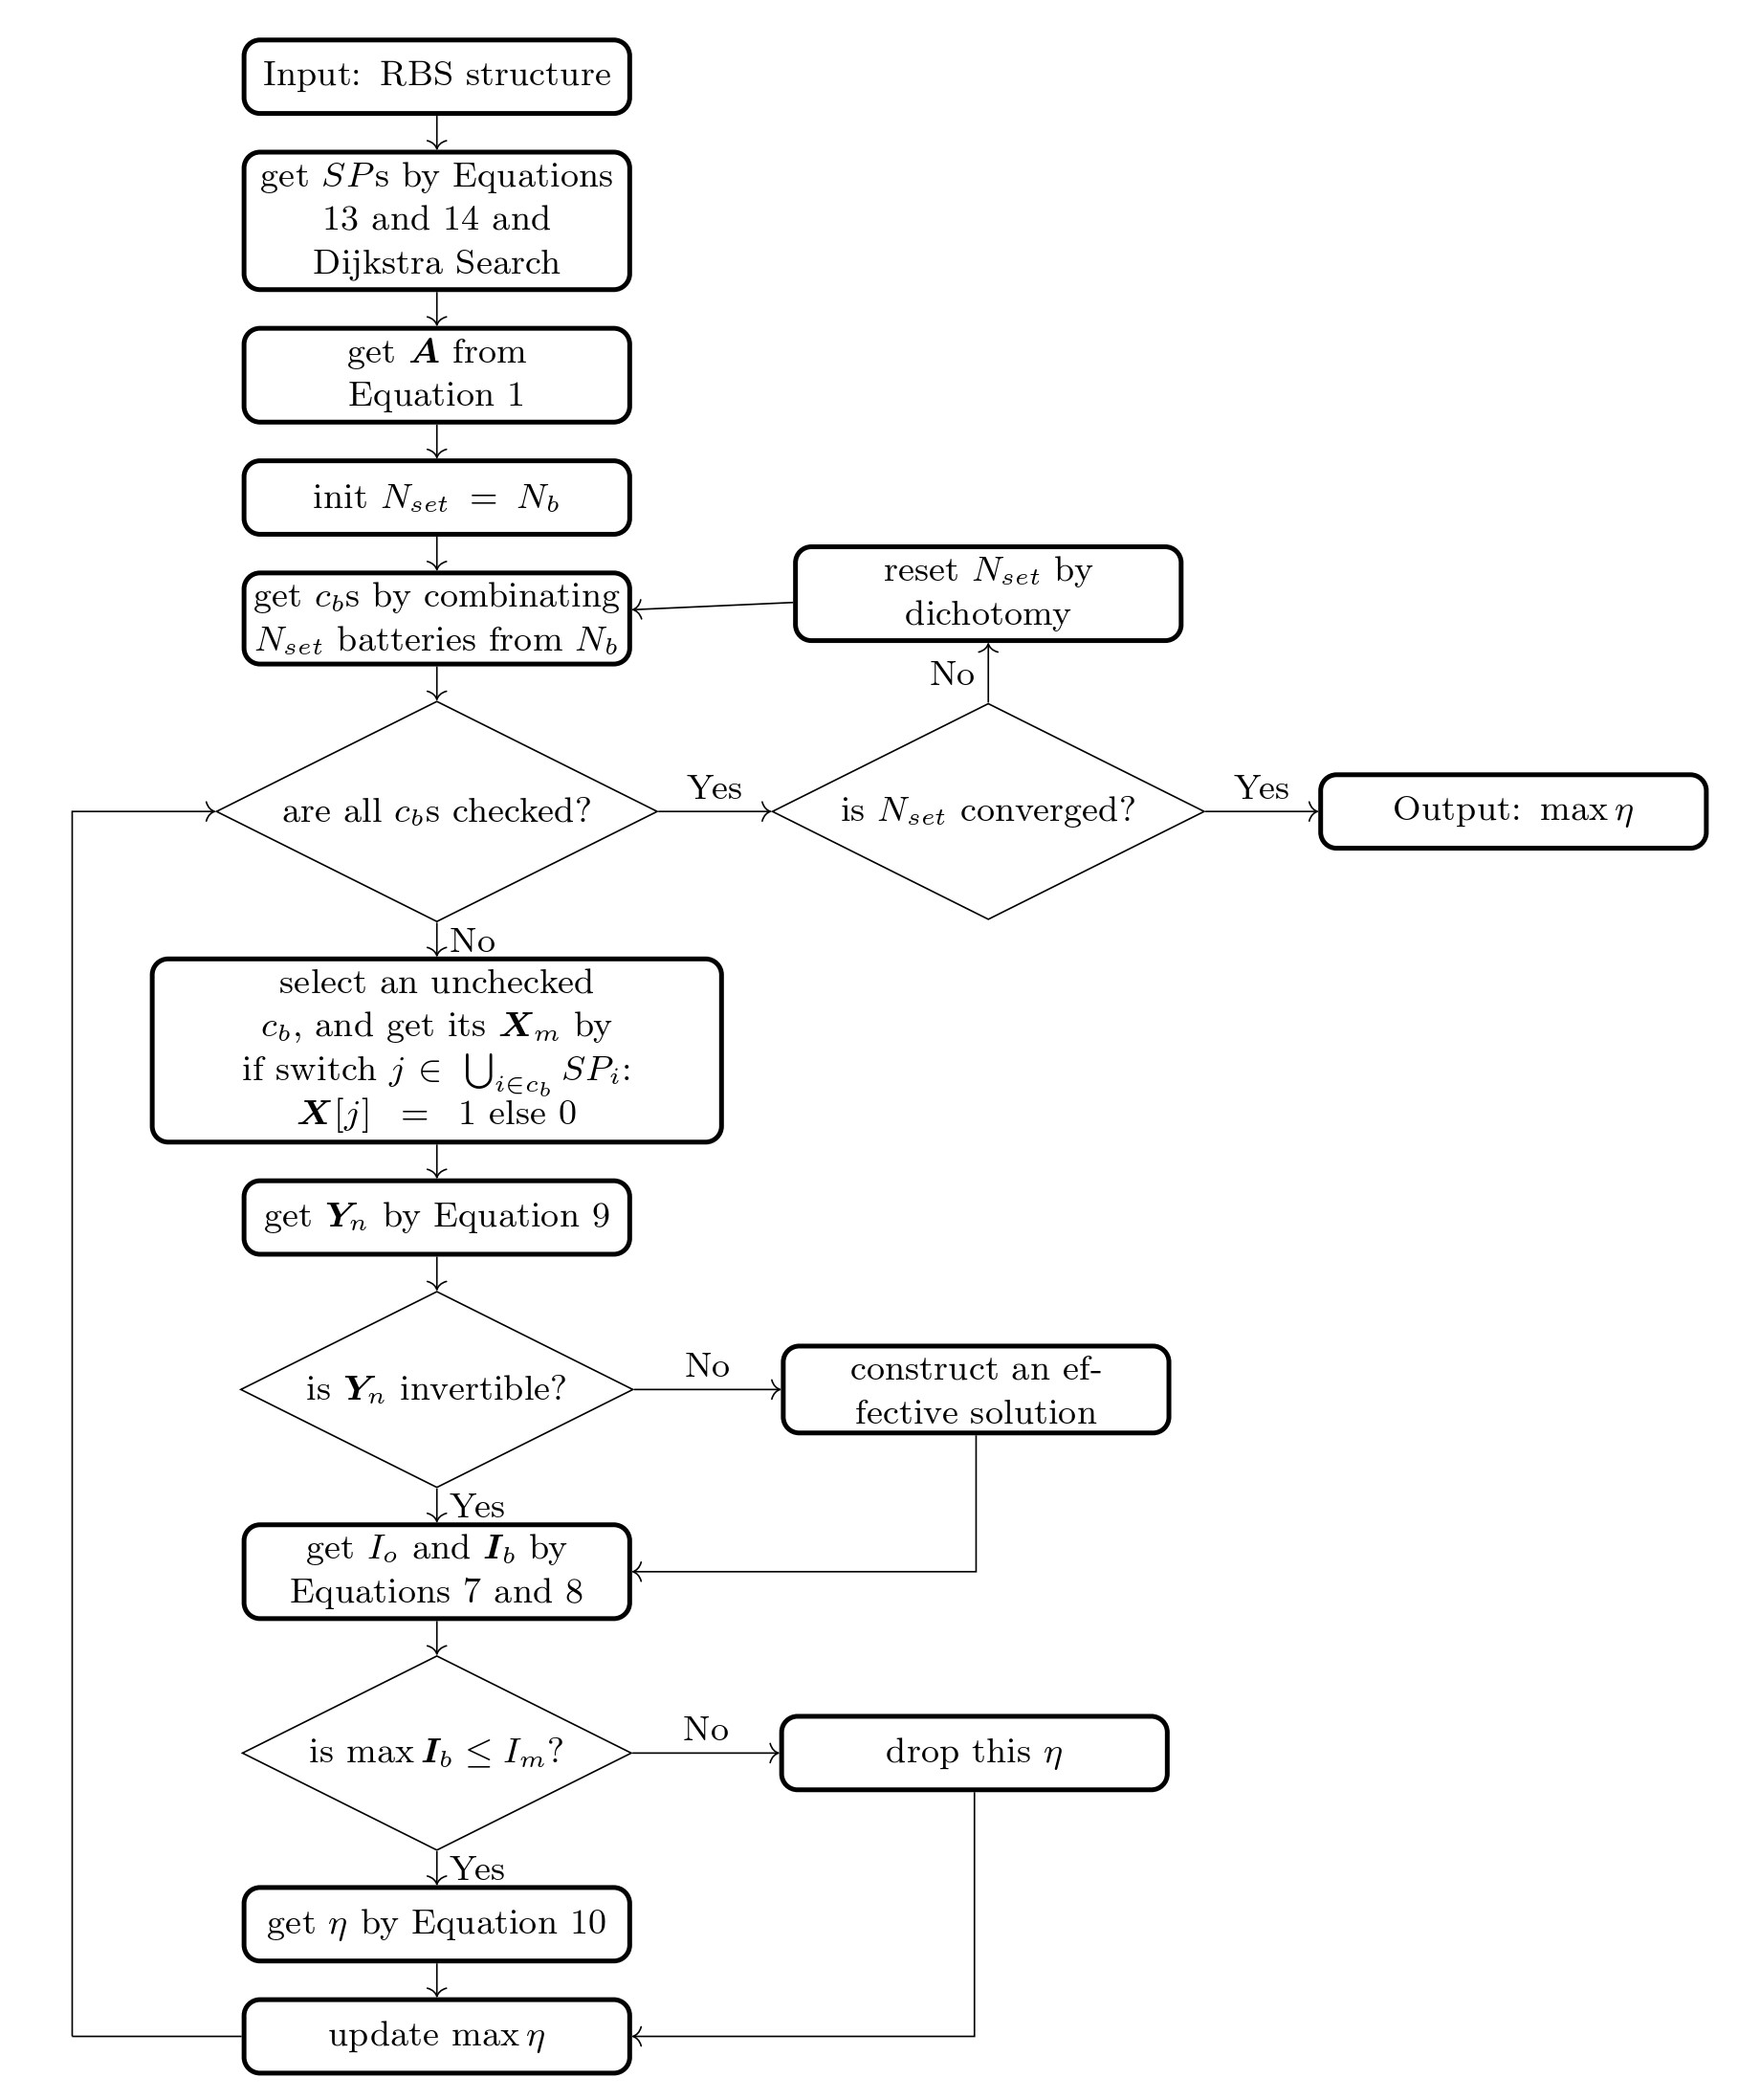
\includegraphics[width=\textwidth]{flowchart.jpg}
%DIF <      \caption{Computational flowchart of MAC for a given RBS.}\label{fig:flowchart}
%DIF <  \end{figure}
\DIFdelbegin %DIFDELCMD < 

%DIFDELCMD < %%%
\DIFdelend \section{Case Study}

\subsection{Structures \DIFaddbegin \DIFadd{and details}\DIFaddend }

\begin{figure}[htbp]
    \centering
    \begin{subfigure}[b]{0.2\textwidth}
        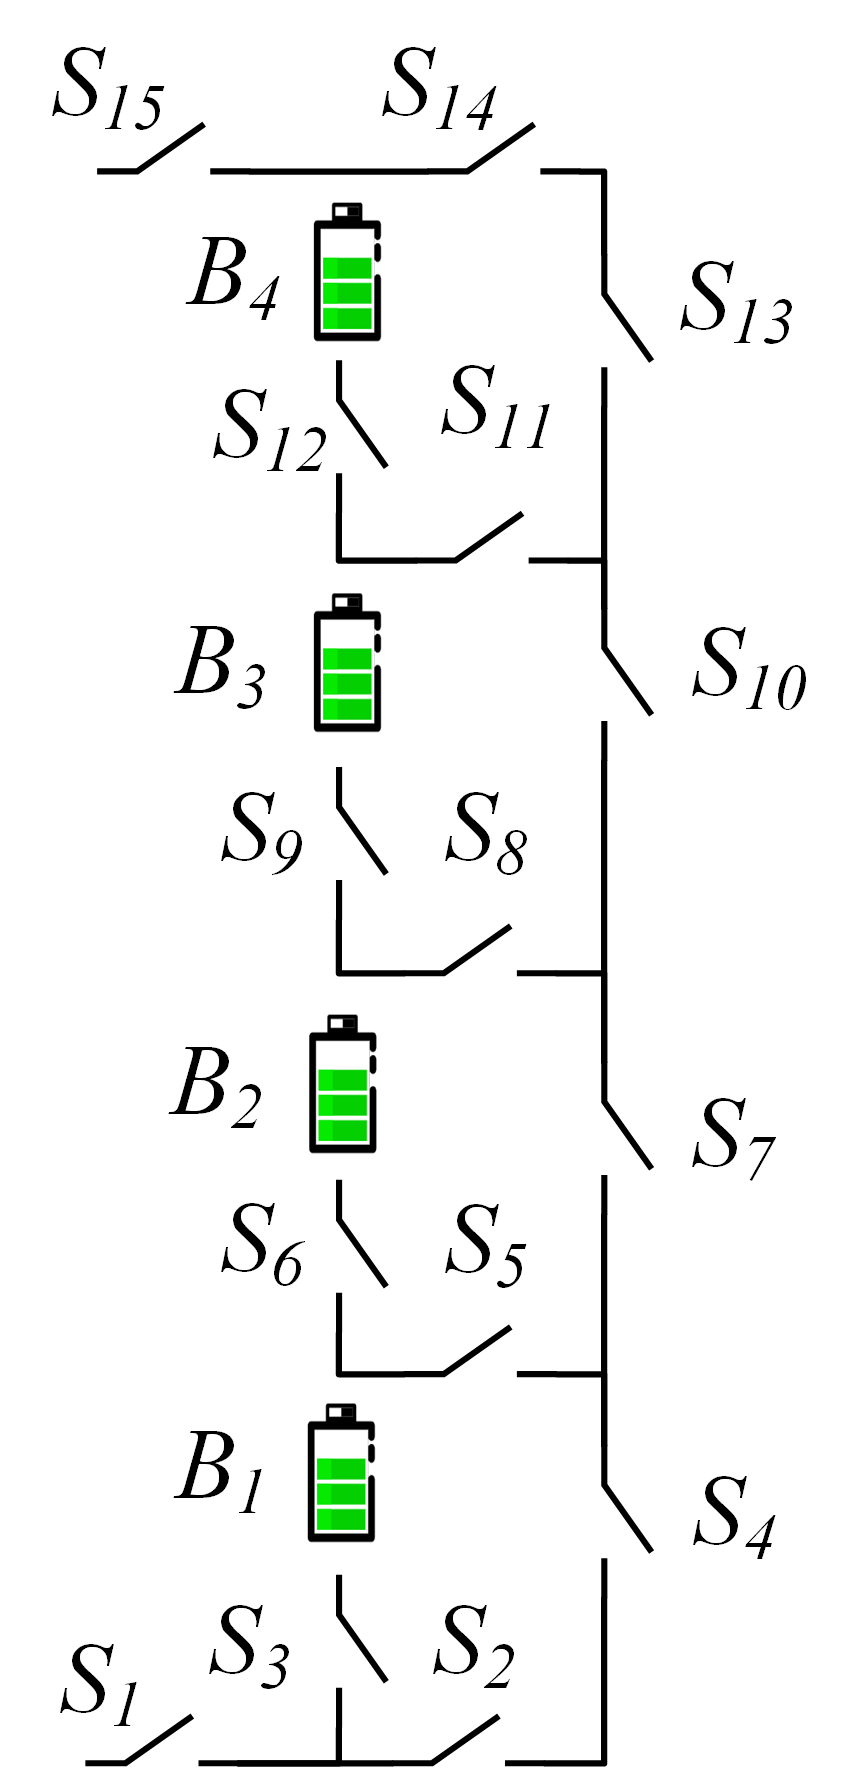
\includegraphics[width=\textwidth]{stru-L-origin.png}
        \caption{}
        \label{fig:study-stru-Lawson}
    \end{subfigure}
    \hspace{0.02\textwidth}
    \begin{subfigure}[b]{0.4\textwidth}
        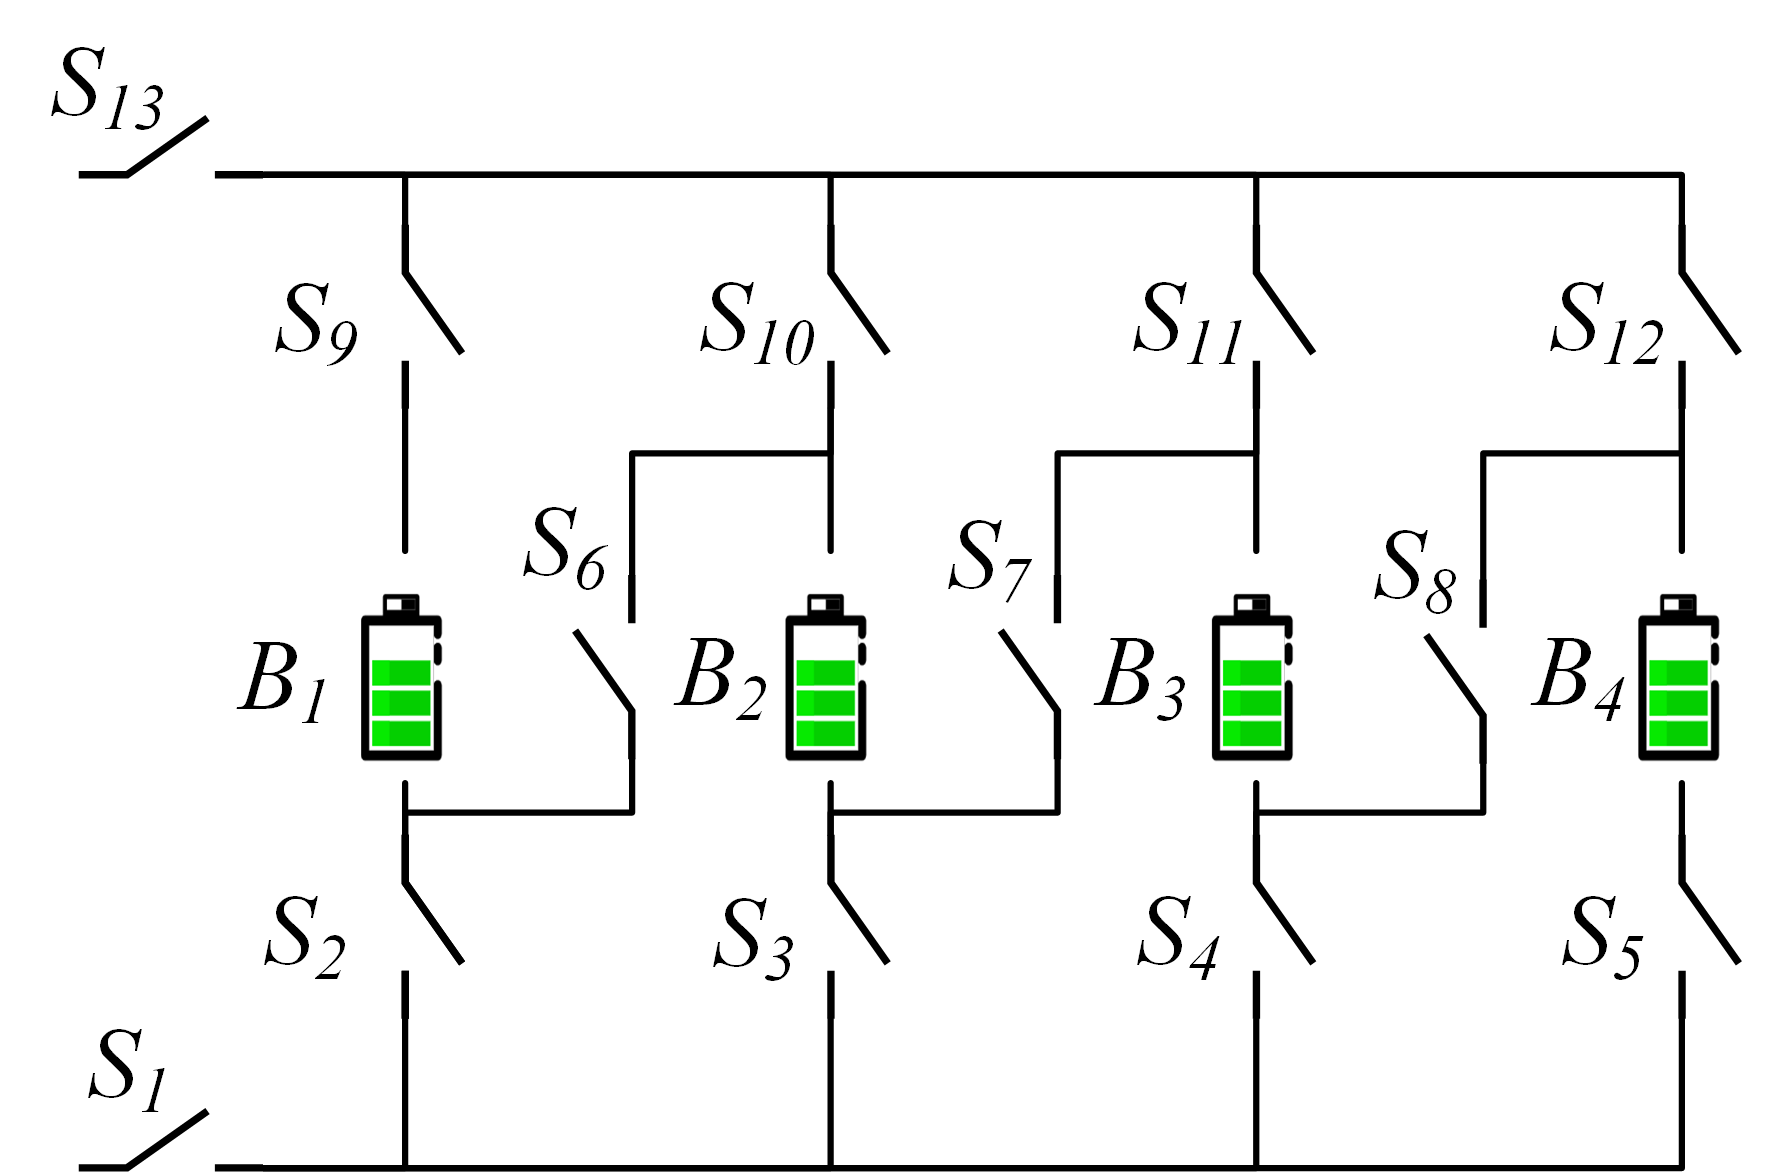
\includegraphics[width=\textwidth]{stru-V-origin.png}
        \caption{}
        \label{fig:study-stru-Visairo}
    \end{subfigure}
    \hspace{0.02\textwidth}
    \begin{subfigure}[b]{0.31\textwidth}
        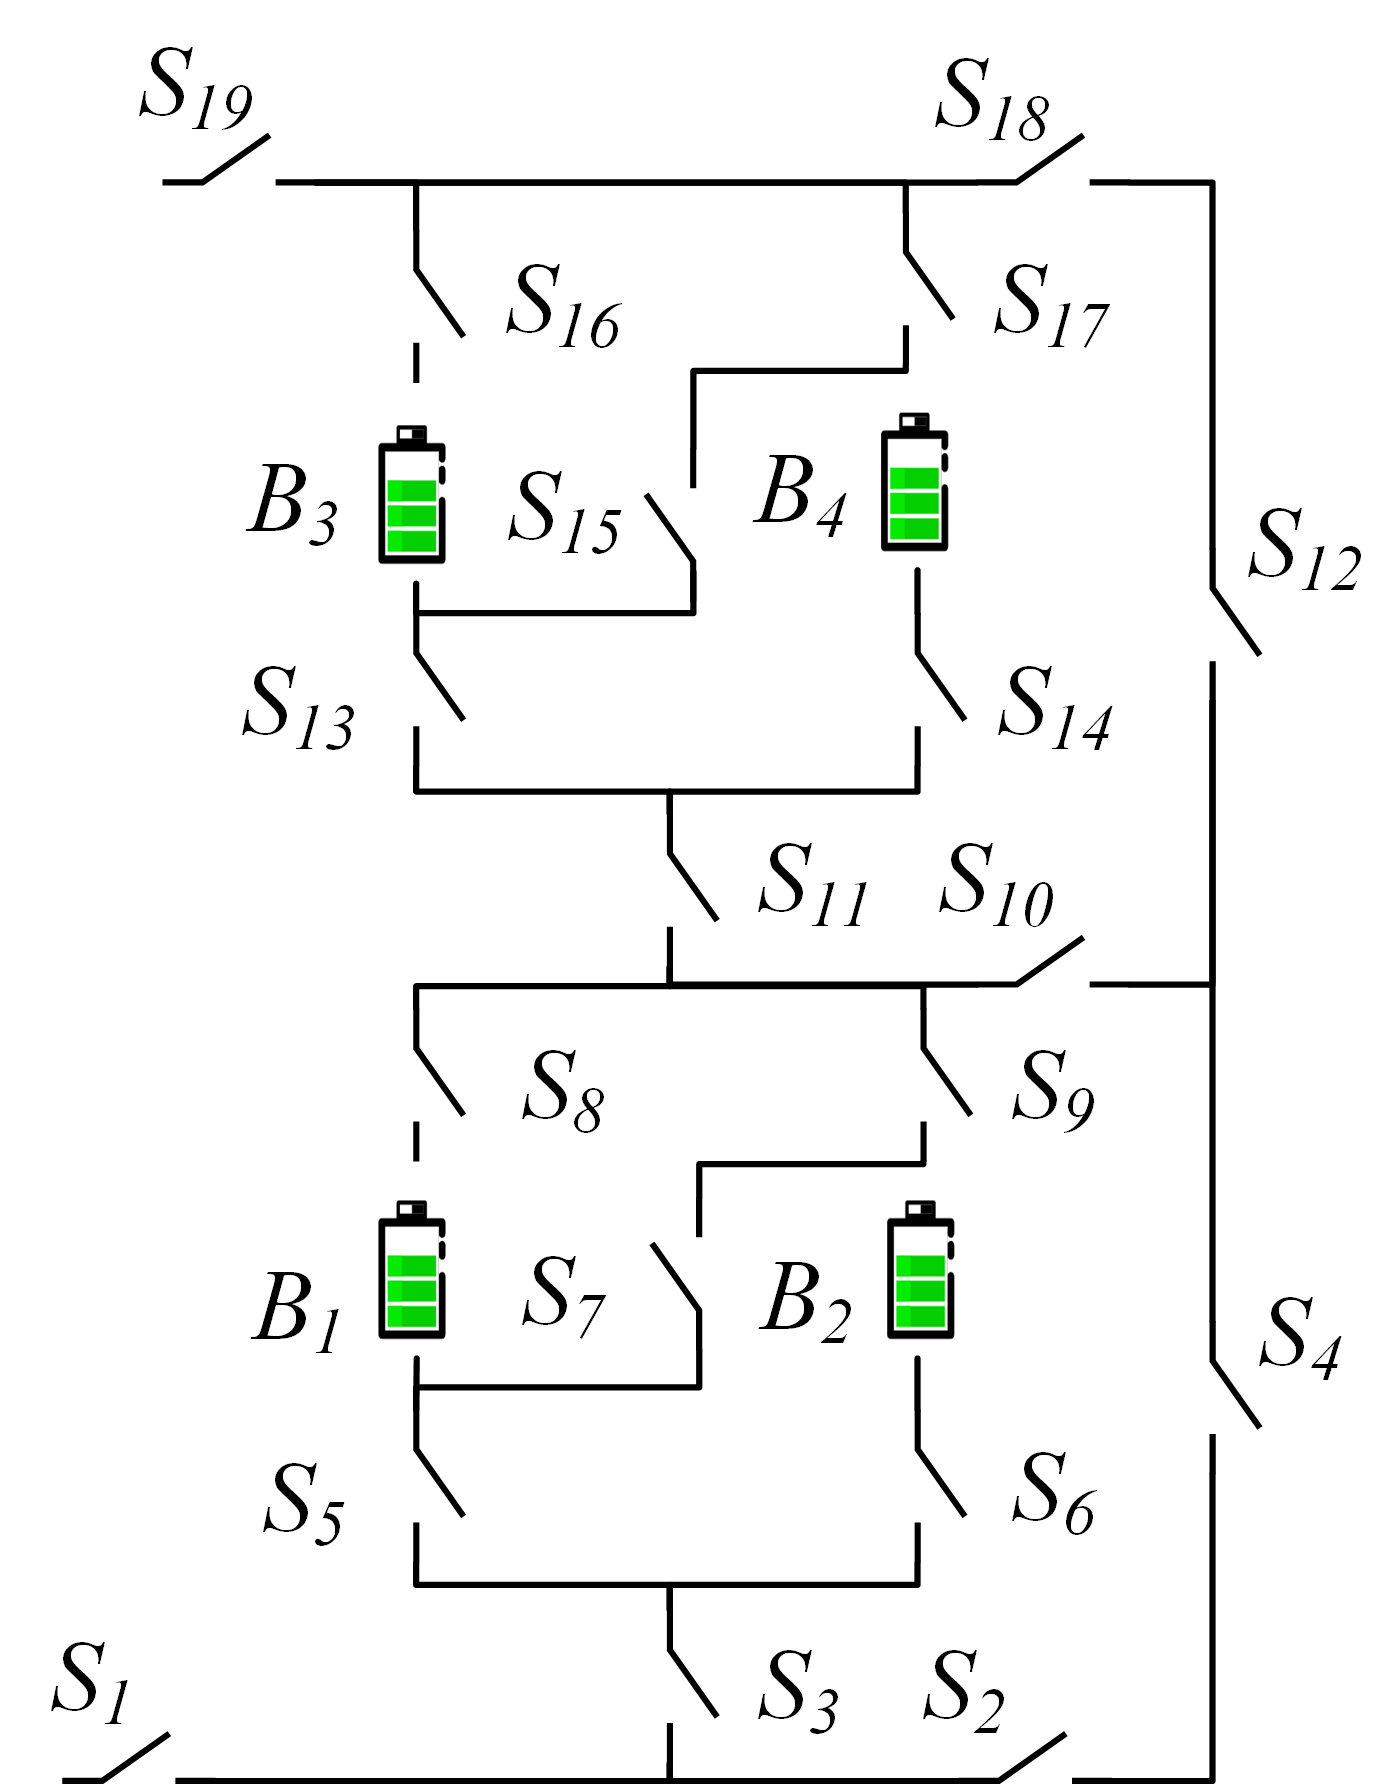
\includegraphics[width=\textwidth]{stru-my-origin.png}
        \caption{}
        \label{fig:study-stru-my}
    \end{subfigure}
    \caption{The four-battery RBS structures proposed by (a) Lawson \cite{lawsonSoftwareConfigurableBattery2012}, (b) Visairo \DIFaddbeginFL \DIFaddFL{and Kumar }\DIFaddendFL \cite{visairoReconfigurableBatteryPack2008}, and (c) this paper.}
\end{figure}

Currently, \DIFaddbegin \DIFadd{there are }\DIFaddend two types of RBS structures \DIFdelbegin \DIFdel{have been proposed by Visairo et al. }\DIFdelend \DIFaddbegin \DIFadd{in the existing literature --- those of Visairo and Kumar }\DIFaddend \cite{visairoReconfigurableBatteryPack2008} and Lawson \DIFdelbegin \DIFdel{et al. }\DIFdelend \cite{lawsonSoftwareConfigurableBattery2012}, both of which have seen real use. 
The primary goal of Visairo \DIFaddbegin \DIFadd{and Kumar}\DIFaddend 's structure (Fig. \ref{fig:study-stru-Visairo}) is to dynamically adjust the RBS output power. However, the isolation of unhealthy batteries is not sufficiently addressed in their work. 
Lawson \DIFdelbegin \DIFdel{et al. }\DIFdelend designed the RBS structure shown in Fig. \ref{fig:study-stru-Lawson} to isolate batteries. 
Although this structure easily isolates batteries, it cannot dynamically adjust the output current of the RBS. 
Based on the \DIFdelbegin \DIFdel{structures }\DIFdelend \DIFaddbegin \DIFadd{structure }\DIFaddend of Visairo and \DIFaddbegin \DIFadd{Kumar and that of }\DIFaddend Lawson, this paper proposes the structure shown in Fig. \ref{fig:study-stru-my}.
By integrating the Visairo \DIFaddbegin \DIFadd{and Kumar }\DIFaddend RBS structure into the Lawson RBS structure, the proposed structure not only has the flexibility to switch the batteries between series, parallel, and mixed series-parallel modes\DIFaddbegin \DIFadd{, }\DIFaddend but also allows the isolation of highly degraded batteries from the RBS.
\DIFdelbegin \DIFdel{These four-battery RBS structures are investigated in }\DIFdelend \DIFaddbegin 


\DIFadd{In }\DIFaddend the case study, \DIFdelbegin \DIFdel{including the scenarios with random isolated batteries.
}%DIFDELCMD < 

%DIFDELCMD < %%%
\subsection{\DIFdel{Result}}
%DIFAUXCMD
\addtocounter{subsection}{-1}%DIFAUXCMD
%DIFDELCMD < 

%DIFDELCMD < %%%
\DIFdel{As shown }\DIFdelend \DIFaddbegin \DIFadd{the following RBS systems are investigated and compared: (a) three different structures (Figs. \ref{fig:study-stru-Lawson}--\ref{fig:study-stru-my}) with the same four batteries; (b) the same structure as }\DIFaddend in Fig. \ref{fig:study-stru-my} \DIFdelbegin \DIFdel{, the new RBS structure consists of fourbatteries }\DIFdelend \DIFaddbegin \DIFadd{with two/four/six batteries; and (c) the four-battery structure in Fig. \ref{fig:study-stru-my} with random isolated batteries. 
The greedy algorithm proposed in this work is also compared with the brute-force algorithm, SA, }\DIFaddend and \DIFdelbegin \DIFdel{19 switches. Figure \ref{fig:study-dirgraph-my} shows the corresponding directed graph, which is composed of 18 nodes and 43 edges. 
Batteries $B_1$, $B_2$, $B_3$, and $B_4$ are denoted by green directed edges in the graph, and the 19 switches are represented by gray directed edges with bidirectional arrows. 
The external electrical load is treated as a directed edge from the cathode of the RBS (i.e., node 18) to the anode (i.e., node }\DIFdelend \DIFaddbegin \DIFadd{GA to validate its effectiveness and efficiency.
In order to adapt the two heuristic algorithms to the system's structure and scale, the number of state neighbors of SA and the population size of GA are both set to $N_b \cdot N_s$, which increases with the number of batteries and switches in the system. 
The parameters of the other algorithms are shown in Tab. \ref{tab:algorithm-parameter}.
}

\begin{table}[htbp]
  \centering
  \caption{\DIFaddFL{The SA and GA algorithm parameters.}}
    \begin{tabular}{lr}
    \toprule
    \DIFaddFL{Algorithm/parameter }& \multicolumn{1}{l}{Value} \\
    \midrule
    \DIFaddFL{SA/initial temperature }& \DIFaddFL{100 }\\
    \DIFaddFL{SA/final temperature }& \DIFaddendFL 1 \DIFdelbeginFL \DIFdelFL{), as indicated by the blue directed edge in the graph. }\DIFdelendFL \DIFaddbeginFL \\
    \DIFaddFL{SA/cooling rate }& \DIFaddFL{0.95 }\\
    \DIFaddFL{GA/total generations }& \DIFaddFL{100 }\\
    \DIFaddFL{GA/crossover probability }& \DIFaddFL{0.8 }\\
    \DIFaddFL{GA/mutation probability }& \DIFaddFL{0.02 }\\
    \bottomrule
    \end{tabular}
  \label{tab:algorithm-parameter}
\end{table}

\subsection{\DIFadd{Result}}

\subsubsection{\DIFadd{The shortest path}}

\DIFaddend Using Eq. (\ref{eq:weight}) and the Dijkstra algorithm, the SPs of the four batteries in the RBS \DIFdelbegin \DIFdel{structure of Fig. \ref{fig:study-stru-my} are highlighted in red in Figs. \ref{fig:sp1} and \ref{fig:sp4}.
Finally, the calculated }\DIFdelend \DIFaddbegin \DIFadd{structures of Figs. \ref{fig:study-stru-Lawson}, \ref{fig:study-stru-Visairo}, and \ref{fig:study-stru-my} are calculated and highlighted with different colors in Figs. \ref{fig:e4-sp}, \ref{fig:f4-sp}, and \ref{fig:e2f2-sp}, respectively.
}

\begin{figure}[htbp]
    \centering
    \begin{subfigure}[b]{0.2\textwidth}
        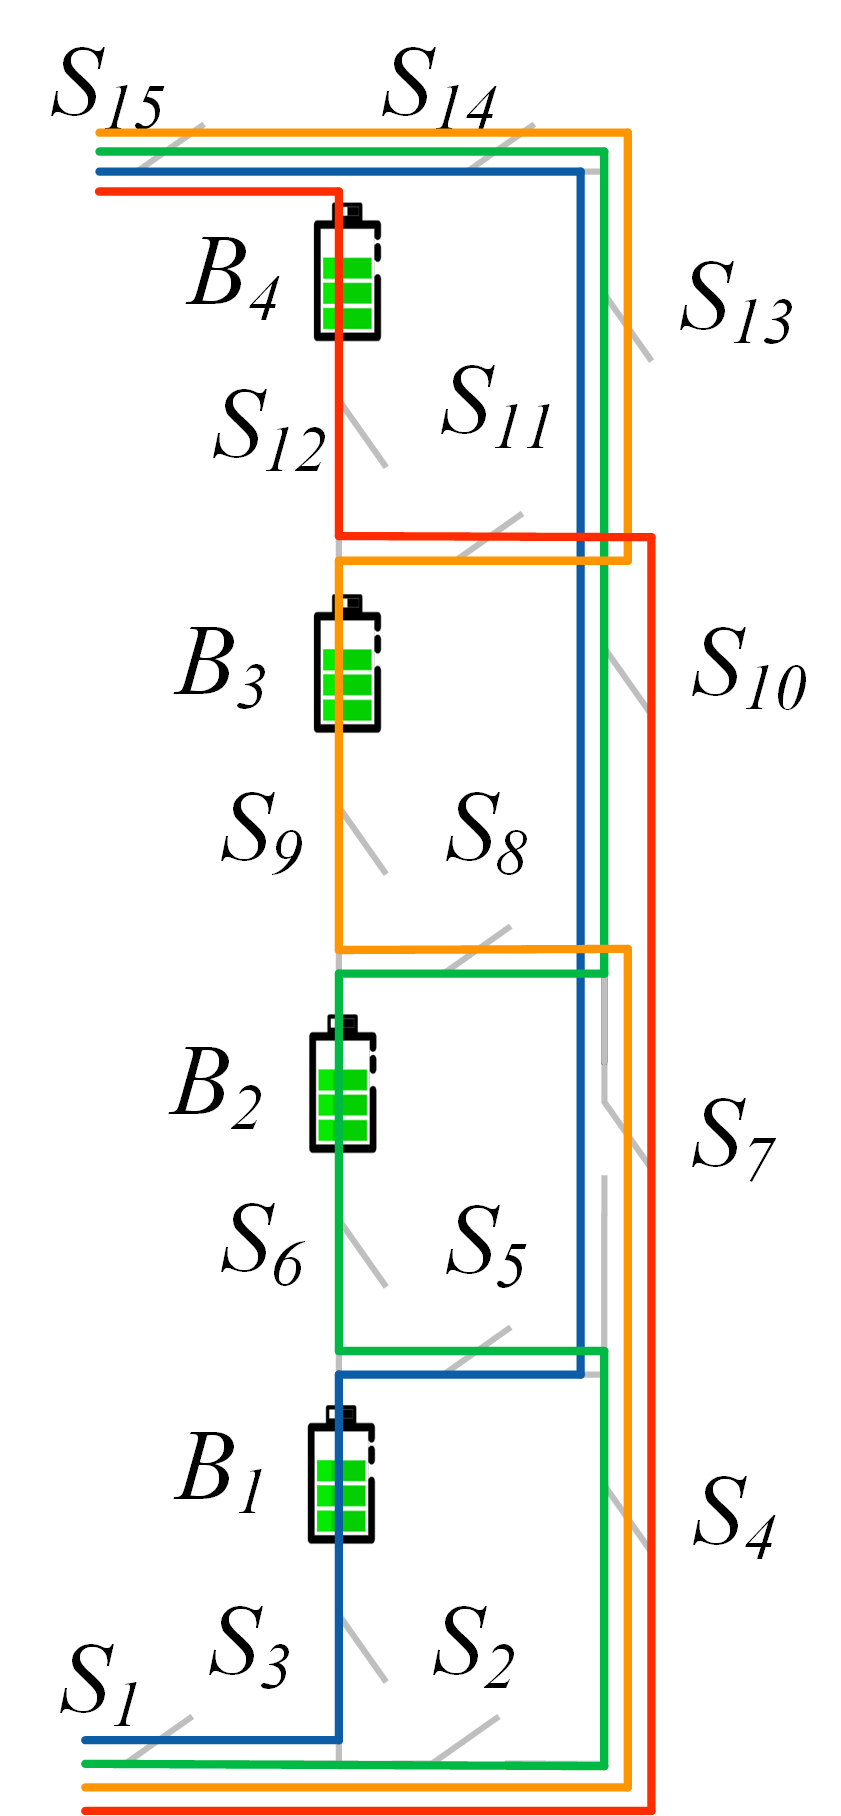
\includegraphics[width=\textwidth]{e4-sp.png}
        \caption{}
        \label{fig:e4-sp}
    \end{subfigure}
    \DIFaddFL{\hspace{0.02\textwidth}
    }\begin{subfigure}[b]{0.4\textwidth}
        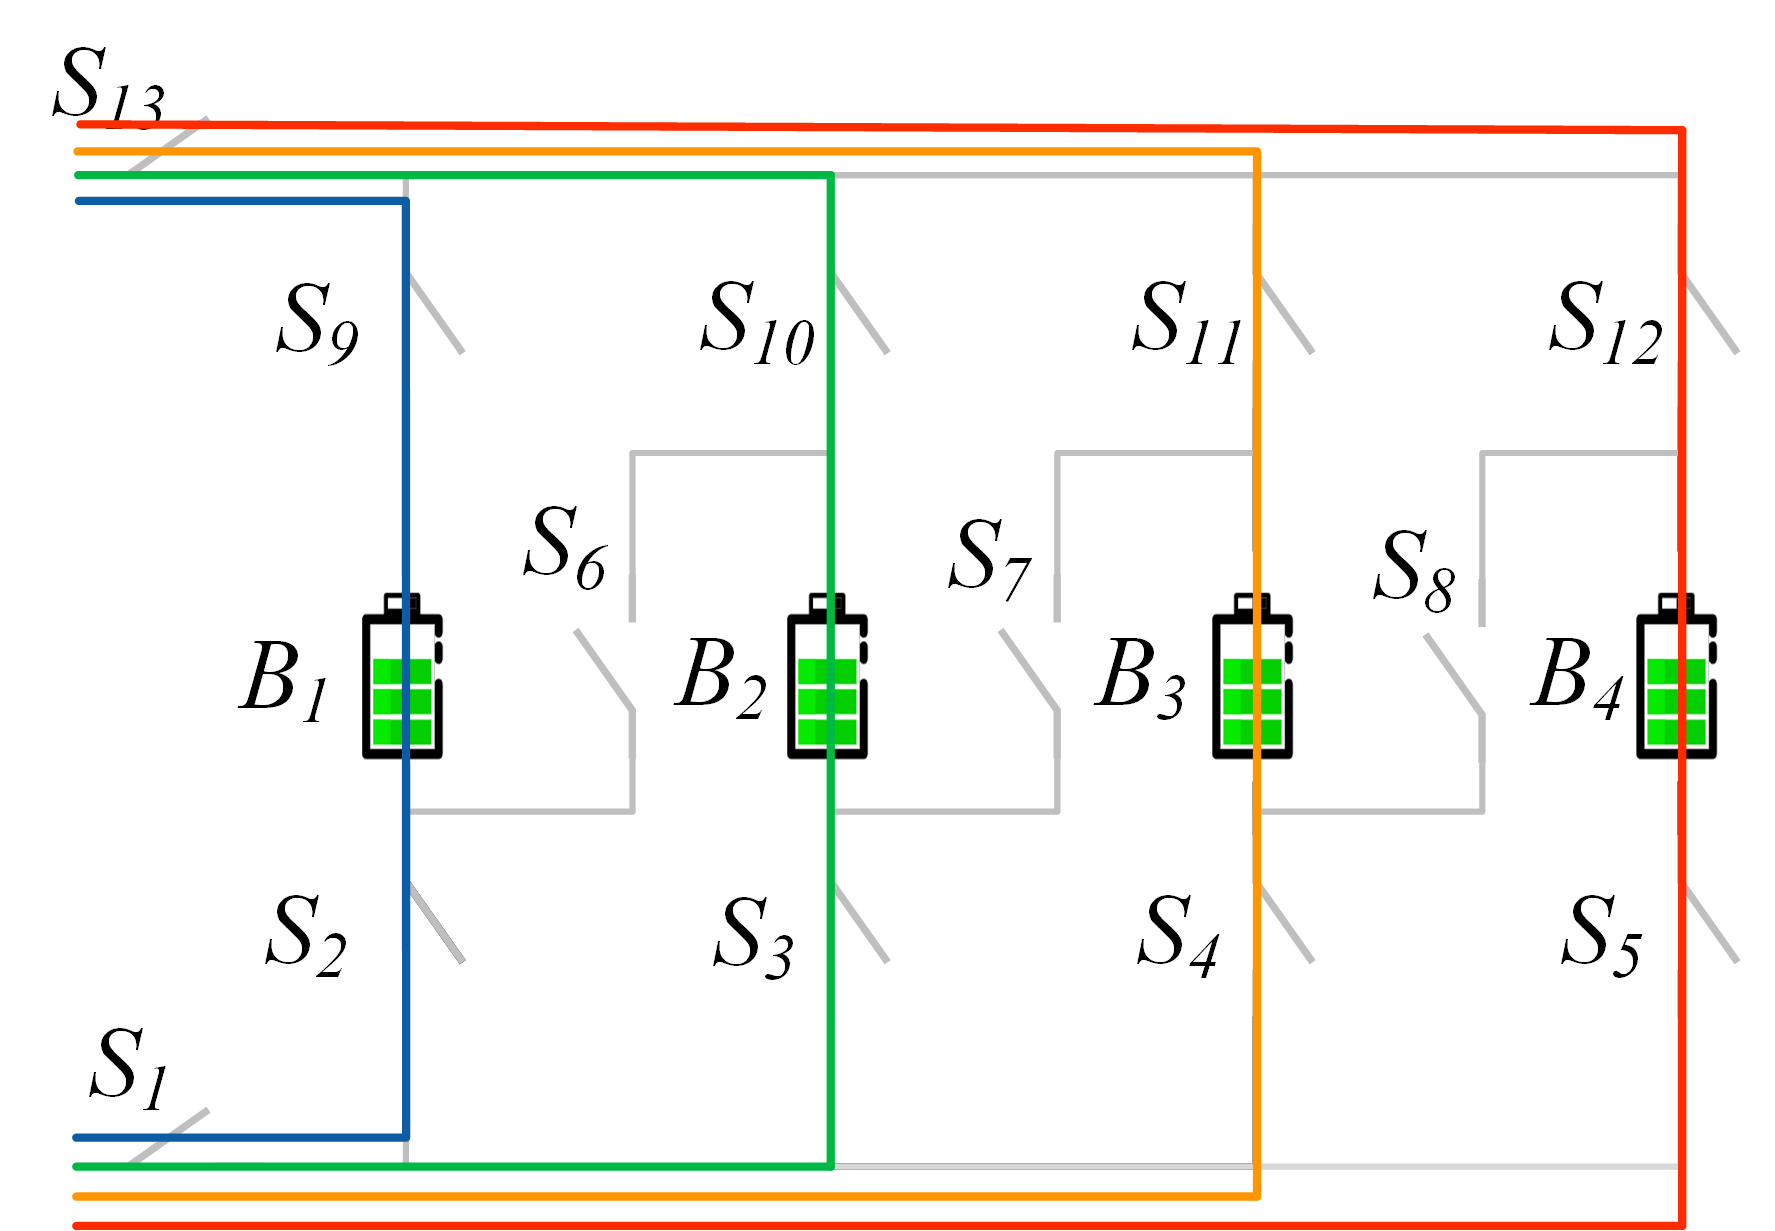
\includegraphics[width=\textwidth]{f4-sp.png}
        \caption{}
        \label{fig:f4-sp}
    \end{subfigure}
    \DIFaddFL{\hspace{0.02\textwidth}
    }\begin{subfigure}[b]{0.31\textwidth}
        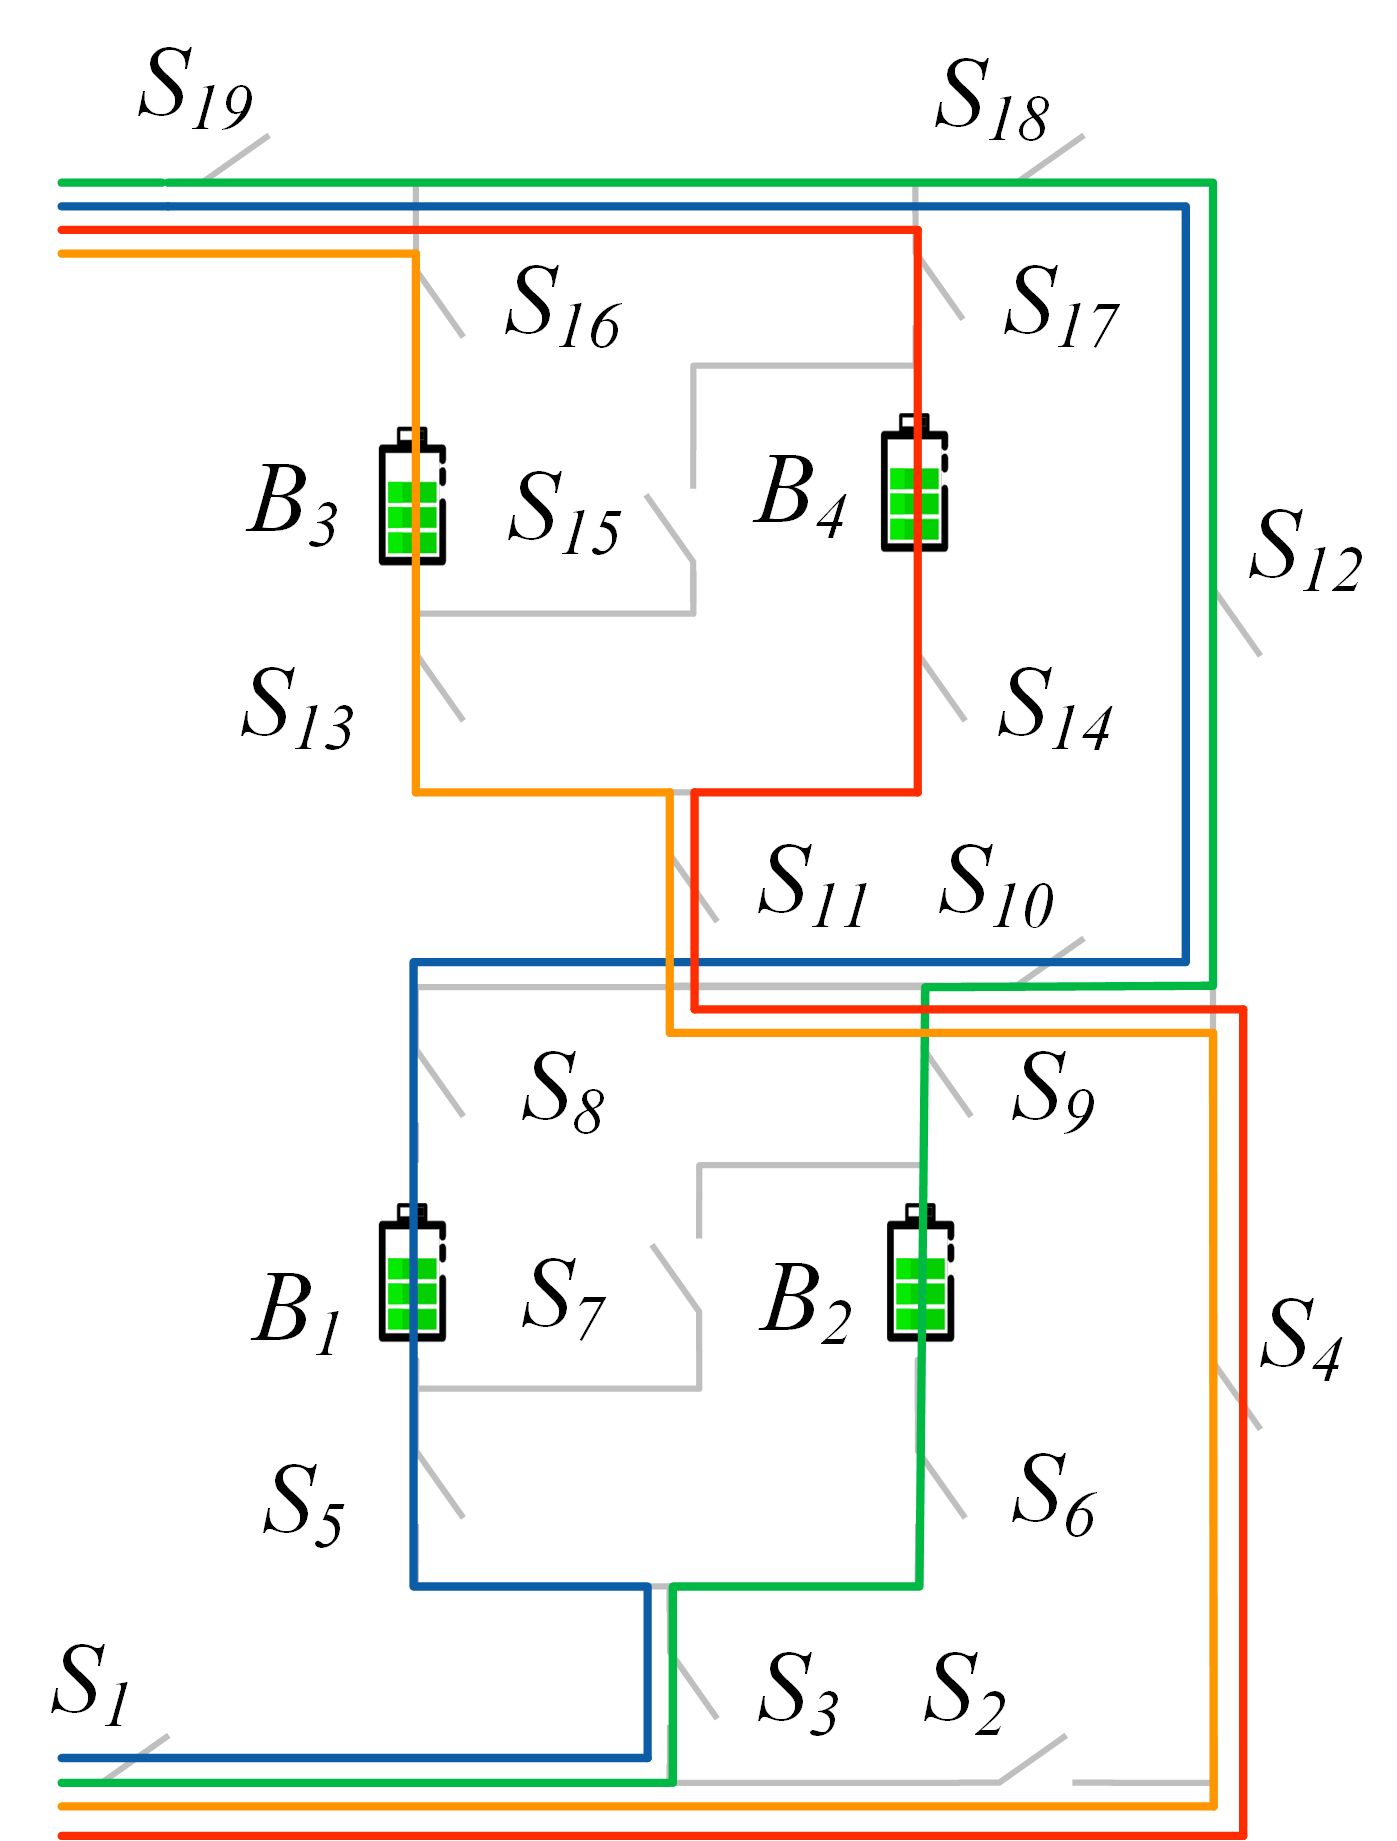
\includegraphics[width=\textwidth]{e2f2-sp.png}
        \caption{}
        \label{fig:e2f2-sp}
    \end{subfigure}
    \caption{\DIFaddFL{The SPs of the four batteries in the RBS structures of (a) Fig. \ref{fig:study-stru-Lawson}, (b) Fig. \ref{fig:study-stru-Visairo}, and (c) Fig. \ref{fig:study-stru-my}.}}
\end{figure}

\subsubsection{\DIFadd{Three structures with four batteries}}

\DIFadd{After obtaining the SPs, the }\DIFaddend MACs of the \DIFdelbegin \DIFdel{structure in Fig. \ref{fig:study-stru-my} are listed in Tab. \ref{tab:study-results-my} and shown in Fig. \ref{fig:study-results-my}, as obtained by the greedy algorithm \ref{alg:greedy}.
Tab. \ref{tab:study-results-my}}\DIFdelend \DIFaddbegin \DIFadd{three RBS structures with four batteries are calculated using the proposed greedy algorithm, and the results are shown in Tabs. \ref{tab:study-results-Lawson}, \ref{tab:study-results-Visairo}, and \ref{tab:study-results-my}, each of which }\DIFaddend contains the states of the switches, the output current $I_o$, the battery current $\bm{I}_b$, and the ratio $\eta$ \DIFdelbegin \DIFdel{of the RBS structure with all batteries in good health when the RBS }\DIFdelend \DIFaddbegin \DIFadd{when the system }\DIFaddend output reaches the MAC.
\DIFdelbegin \DIFdel{Fig. \ref{fig:study-results-my} presents the corresponding circuit, with the red highlight indicating that the current is flowing through the respective branches.
}%DIFDELCMD < 

%DIFDELCMD < \begin{figure}[htbp]
%DIFDELCMD <     \centering
%DIFDELCMD <     \begin{subfigure}[b]{0.28\textwidth}
%DIFDELCMD <         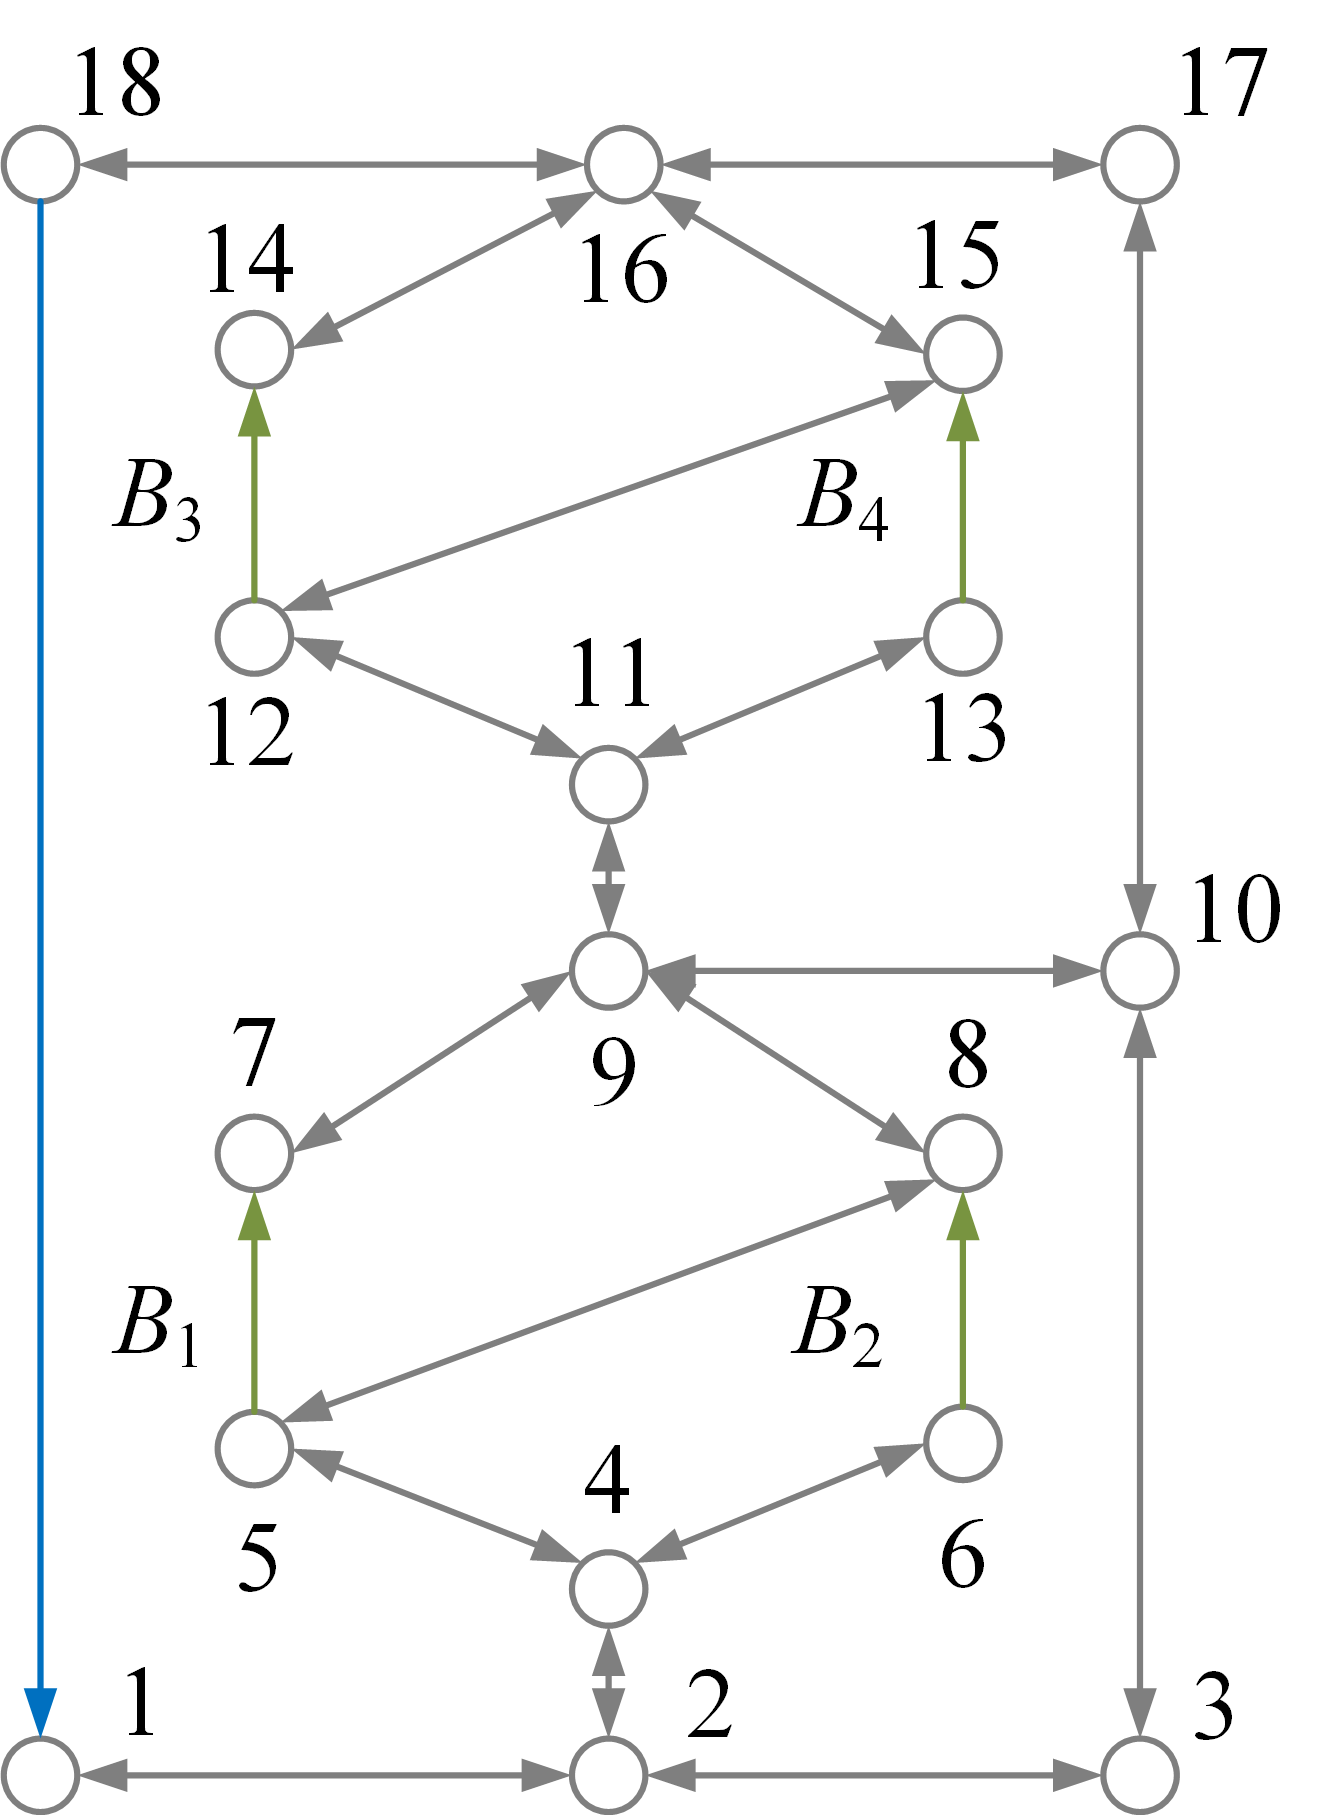
\includegraphics[width=\textwidth]{ef-topo.png}
%DIFDELCMD <         %%%
%DIFDELCMD < \caption{%
{%DIFAUXCMD
}
        %DIFAUXCMD
%DIFDELCMD < \label{fig:study-dirgraph-my}
%DIFDELCMD <     \end{subfigure}
%DIFDELCMD <     %%%
\DIFdelFL{\hspace{0.05\textwidth}
    }%DIFDELCMD < \begin{subfigure}[b]{0.28\textwidth}
%DIFDELCMD <         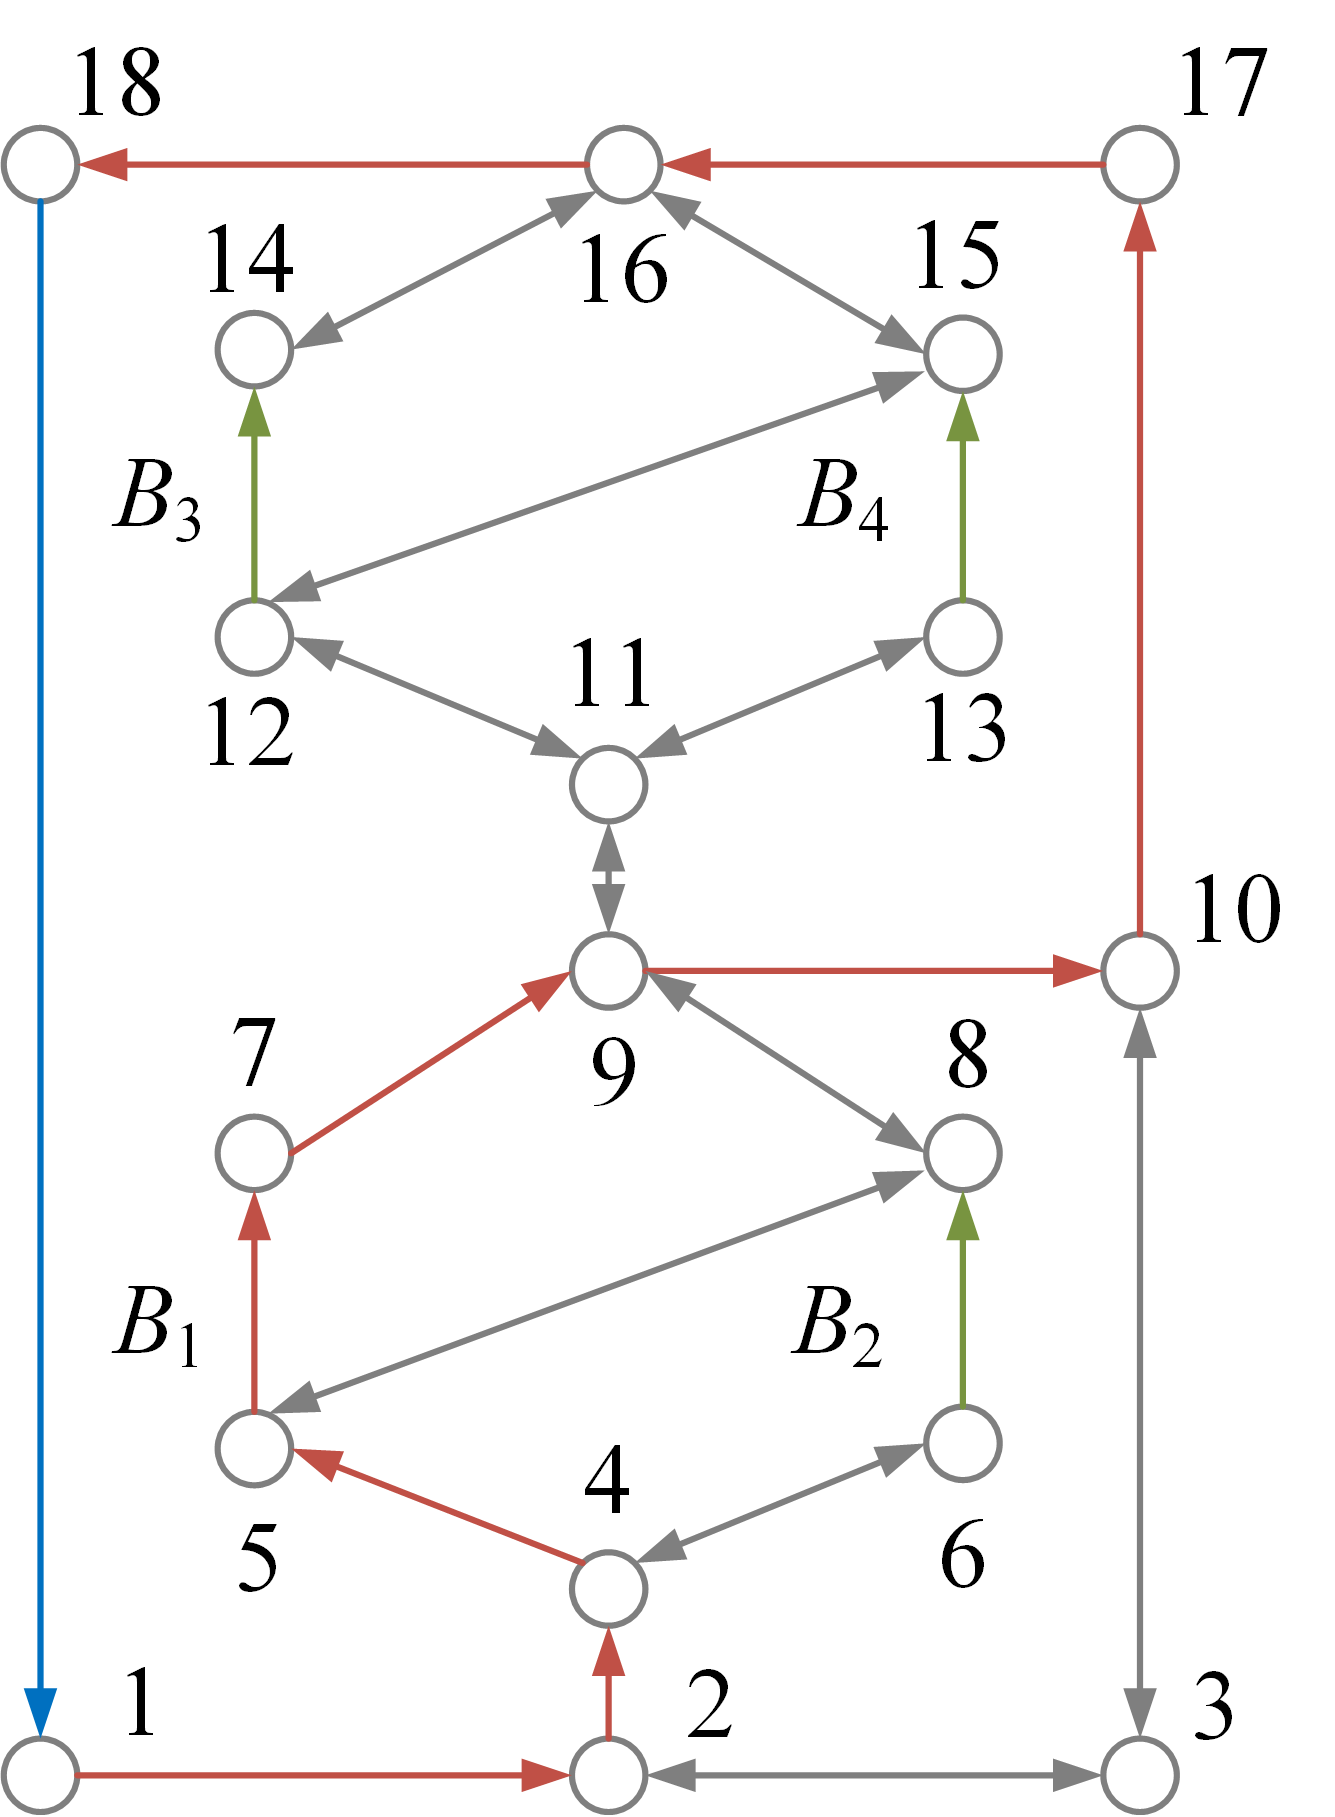
\includegraphics[width=\textwidth]{ef-sp1.png}
%DIFDELCMD <         %%%
%DIFDELCMD < \caption{%
{%DIFAUXCMD
}
        %DIFAUXCMD
%DIFDELCMD < \label{fig:sp1}
%DIFDELCMD <     \end{subfigure}
%DIFDELCMD <     %%%
\DIFdelFL{\hspace{0.05\textwidth}
    }%DIFDELCMD < \begin{subfigure}[b]{0.28\textwidth}
%DIFDELCMD <         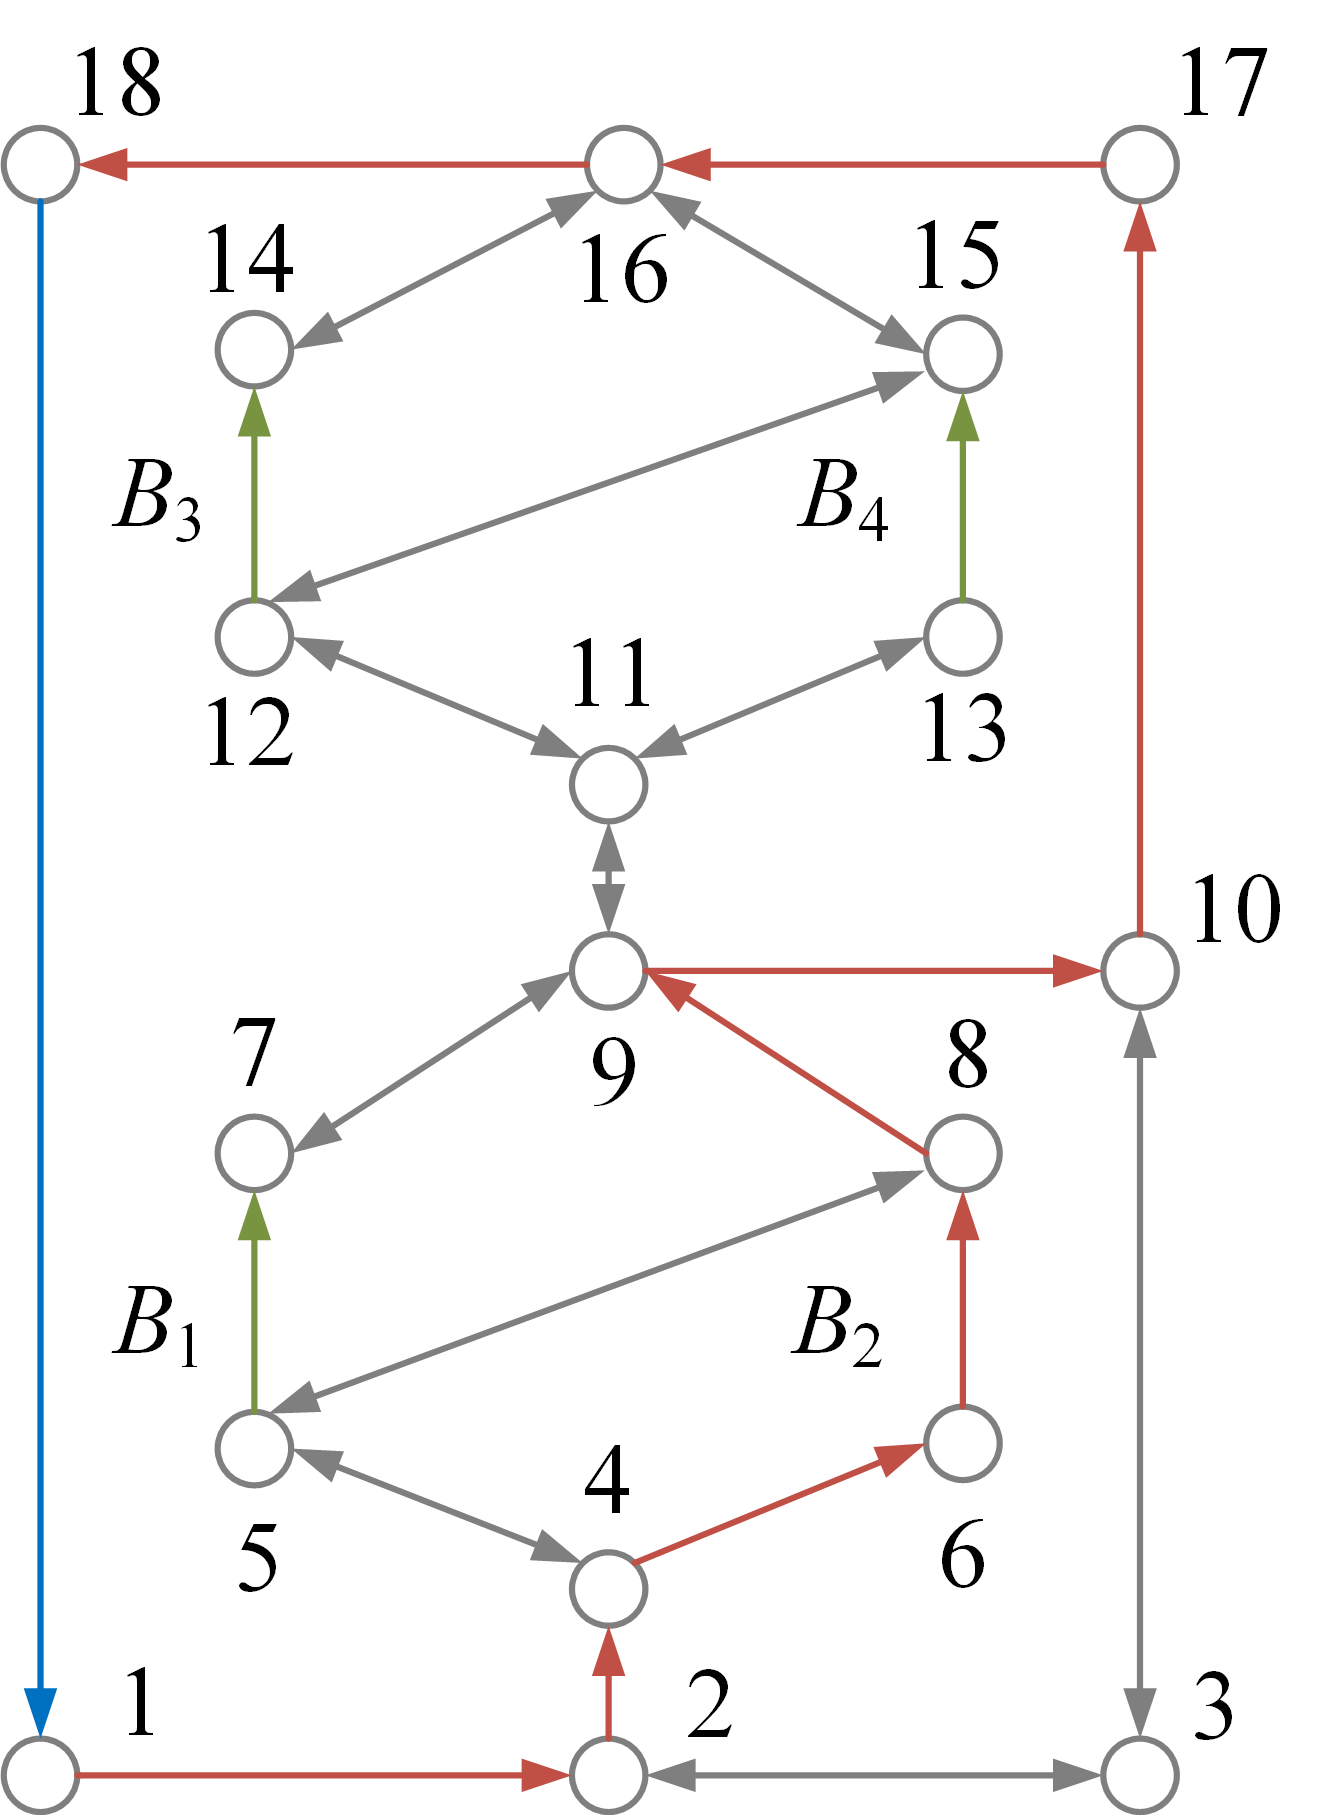
\includegraphics[width=\textwidth]{ef-sp2.png}
%DIFDELCMD <         %%%
%DIFDELCMD < \caption{%
{%DIFAUXCMD
}
        %DIFAUXCMD
%DIFDELCMD < \label{fig:sp2}
%DIFDELCMD <     \end{subfigure}
%DIFDELCMD <     \\
%DIFDELCMD <     \begin{subfigure}[b]{0.28\textwidth}
%DIFDELCMD <         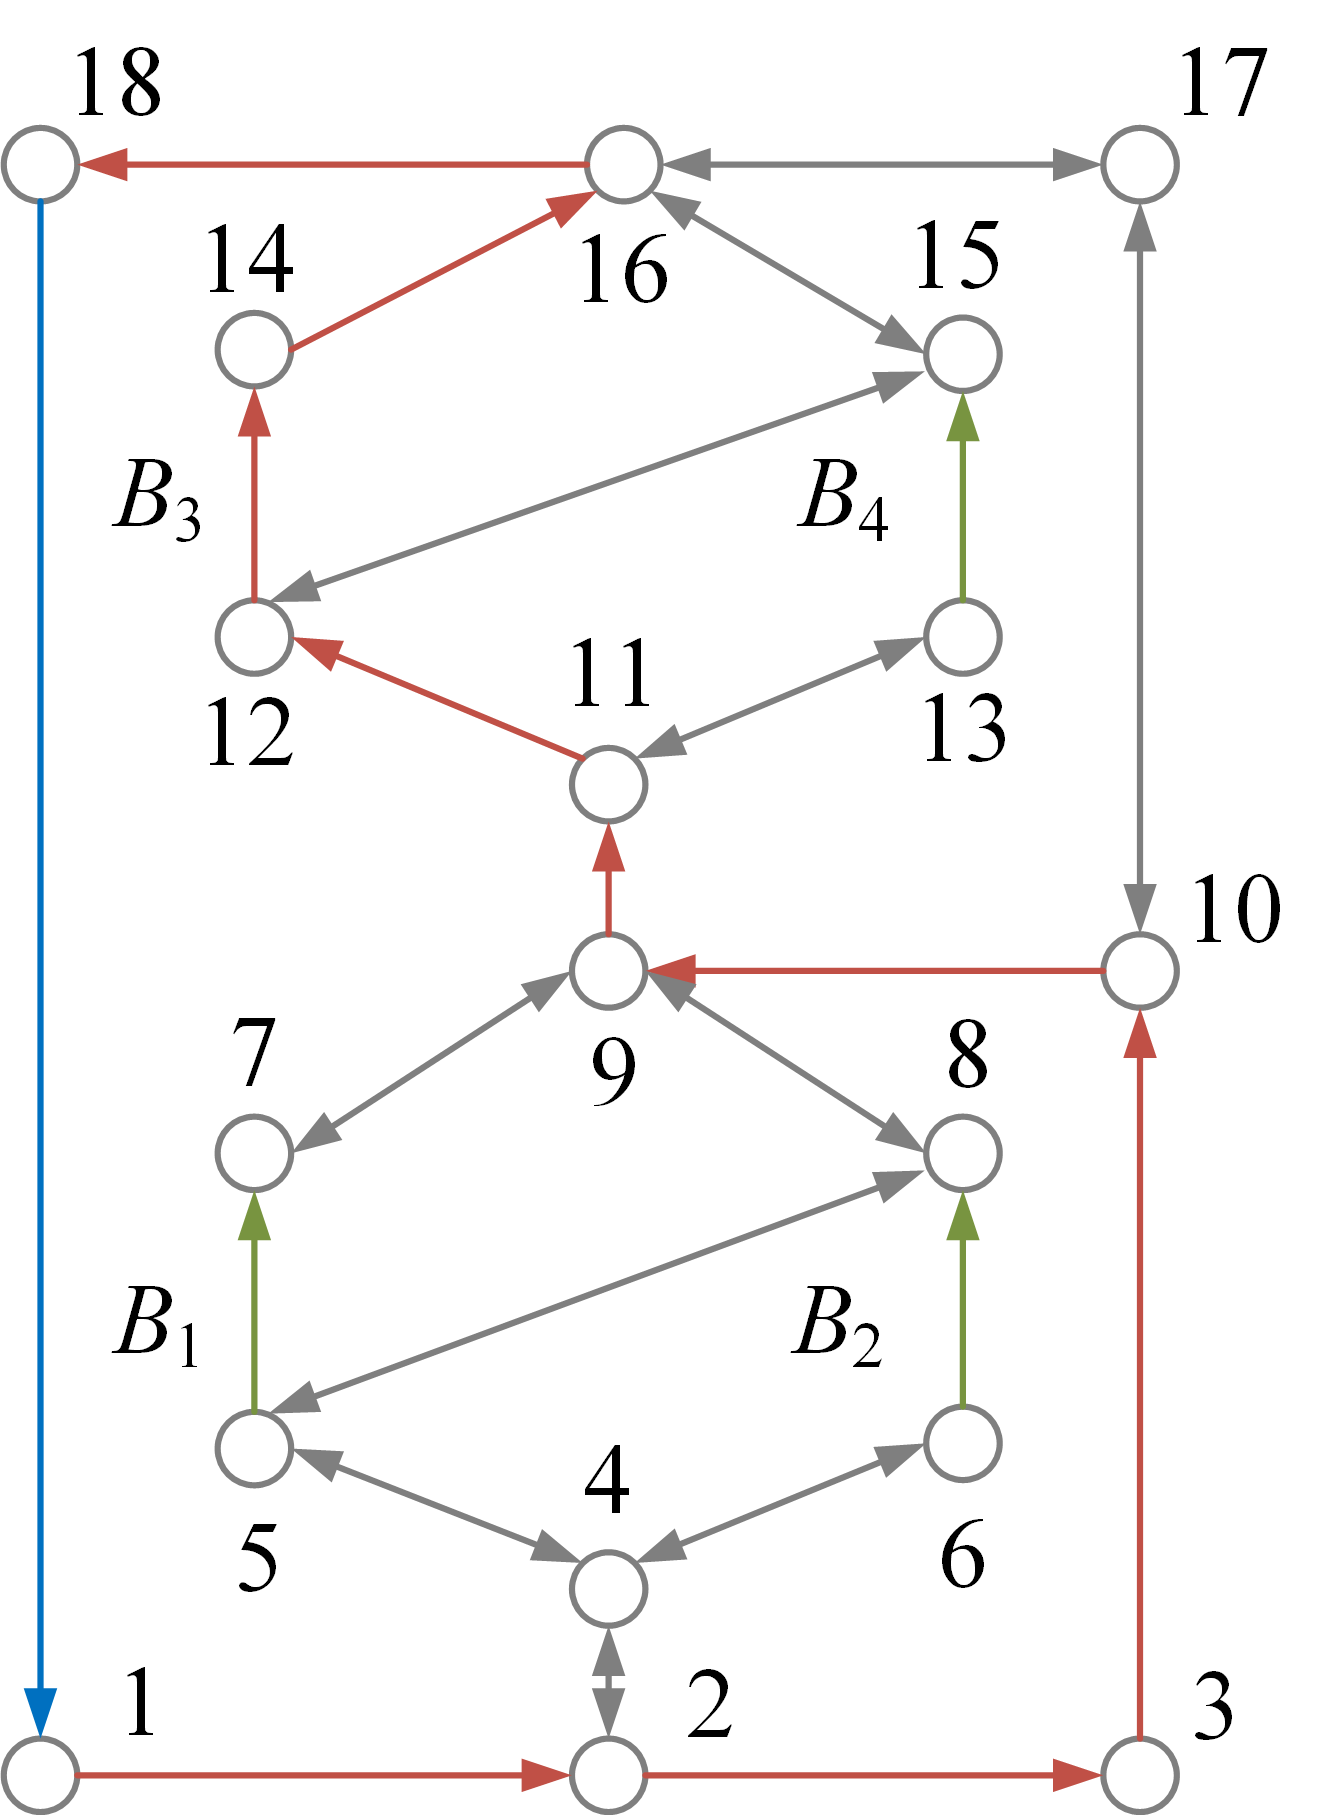
\includegraphics[width=\textwidth]{ef-sp3.png}
%DIFDELCMD <         %%%
%DIFDELCMD < \caption{%
{%DIFAUXCMD
}
        %DIFAUXCMD
%DIFDELCMD < \label{fig:sp3}
%DIFDELCMD <     \end{subfigure}
%DIFDELCMD <     %%%
\DIFdelFL{\hspace{0.05\textwidth}
    }%DIFDELCMD < \begin{subfigure}[b]{0.28\textwidth}
%DIFDELCMD <         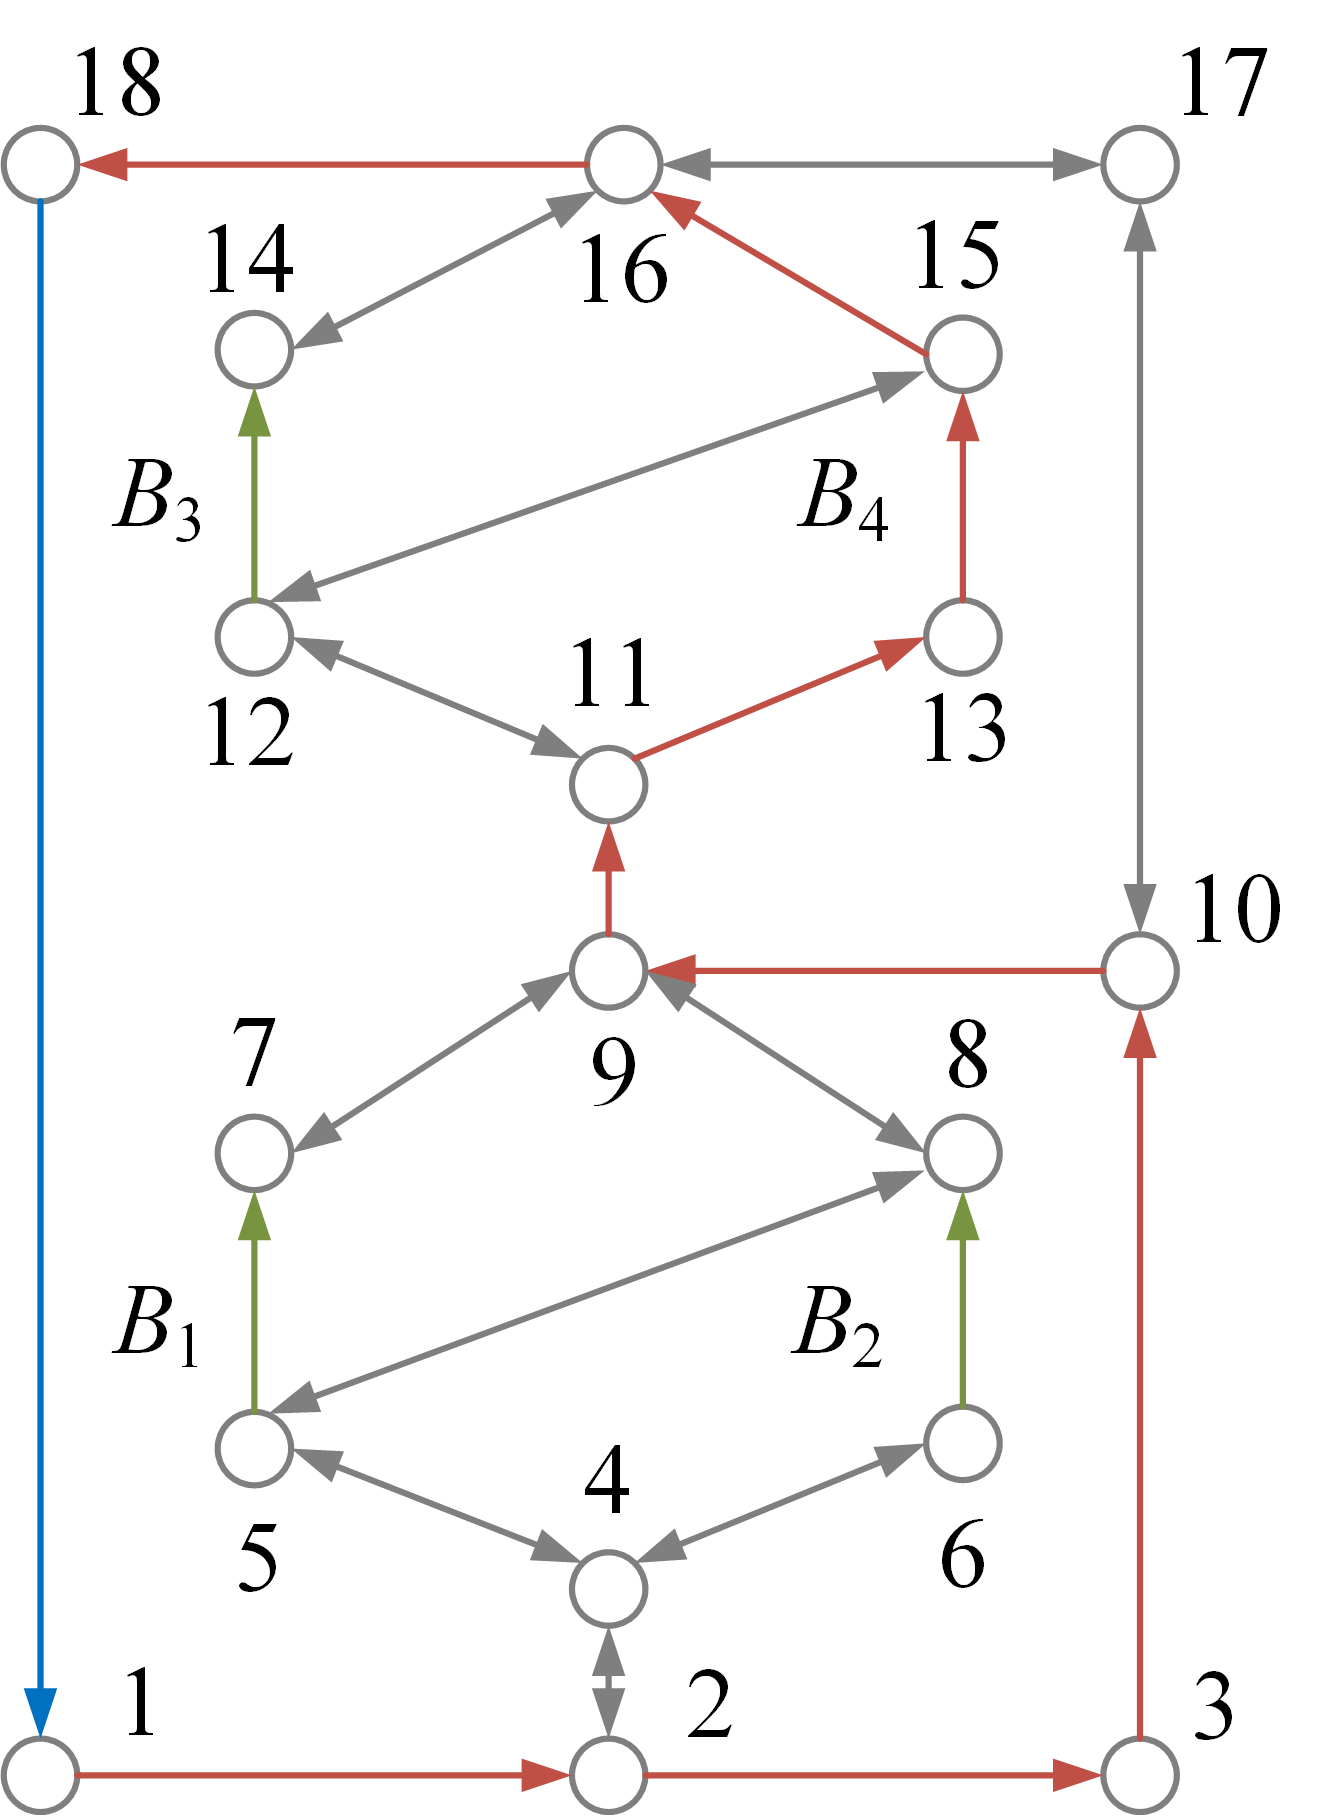
\includegraphics[width=\textwidth]{ef-sp4.png}
%DIFDELCMD <         %%%
%DIFDELCMD < \caption{%
{%DIFAUXCMD
}
        %DIFAUXCMD
%DIFDELCMD < \label{fig:sp4}
%DIFDELCMD <     \end{subfigure}
%DIFDELCMD <     %%%
\DIFdelFL{\hspace{0.05\textwidth}
    }%DIFDELCMD < \begin{subfigure}[b]{0.28\textwidth}
%DIFDELCMD <         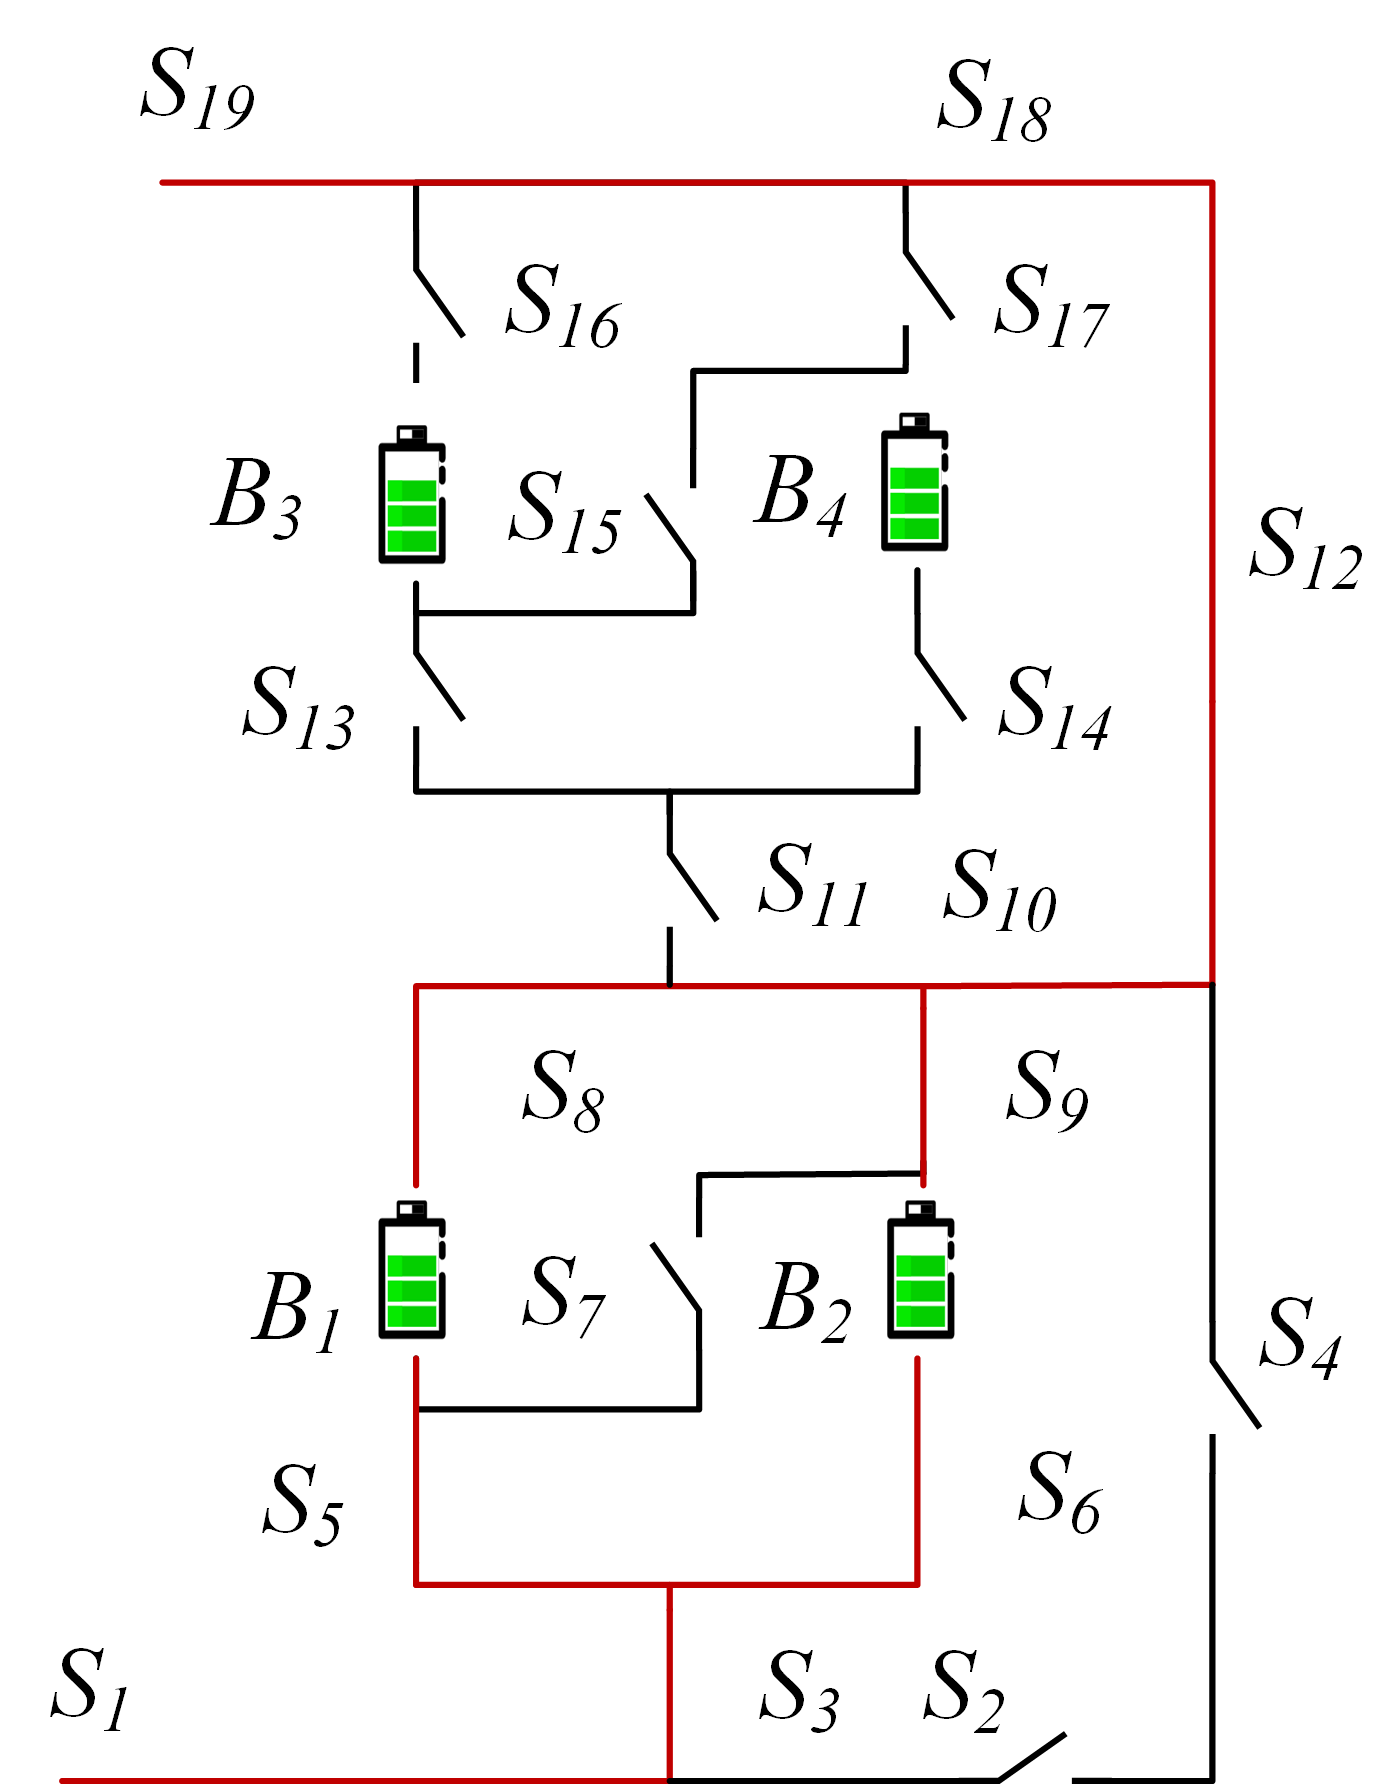
\includegraphics[width=\textwidth]{ef-mac.png}
%DIFDELCMD <         %%%
%DIFDELCMD < \caption{%
{%DIFAUXCMD
}
        %DIFAUXCMD
%DIFDELCMD < \label{fig:study-results-my}
%DIFDELCMD <     \end{subfigure}
%DIFDELCMD <     %%%
%DIFDELCMD < \caption{%
{%DIFAUXCMD
\DIFdelFL{For the RBS structure in Fig. \ref{fig:study-stru-my}, 
        (a) its directed graph 
        and the SPs (highlighted in red) of battery (b) $B_1$, (c) $B_2$, (d) $B_3$, and (e) $B_4$.
        (f) Circuit of RBS with its output reaching the MAC.
        }}
    %DIFAUXCMD
%DIFDELCMD < \label{fig:all-results-my}
%DIFDELCMD < \end{figure}
%DIFDELCMD < 

%DIFDELCMD < \begin{table}[htbp]
%DIFDELCMD <   \centering
%DIFDELCMD <     %%%
%DIFDELCMD < \caption{%
{%DIFAUXCMD
\DIFdelFL{Calculated MAC for four-battery RBS structure in Fig. \ref{fig:study-stru-my}.}}
    %DIFAUXCMD
%DIFDELCMD < \begin{tabular}{cc}
%DIFDELCMD <     \toprule
%DIFDELCMD <         %%%
\DIFdelFL{Structure }%DIFDELCMD < & %%%
\DIFdelFL{Figure \ref{fig:study-stru-my} with four batteries and 19 switches  }%DIFDELCMD < \\
%DIFDELCMD <     \midrule
%DIFDELCMD <     %%%
\DIFdelFL{Switch on }%DIFDELCMD < & %%%
\DIFdelFL{$S_1$,$S_3$,$S_5$,$S_6$,$S_8$,$S_9$,$S_{10}$,$S_{12}$,$S_{18}$,$S_{19}$ }%DIFDELCMD < \\
%DIFDELCMD <     %%%
\DIFdelFL{$I_o$ }%DIFDELCMD < & %%%
\DIFdelFL{$2u_b/(2R_o+r_b)$ }%DIFDELCMD < \\
%DIFDELCMD <     %%%
\DIFdelFL{$\bm{I}_b$ }%DIFDELCMD < & %%%
\DIFdelFL{$[u_b/(2R_o+r_b),u_b/(2R_o+r_b),0,0]$ }%DIFDELCMD < \\
%DIFDELCMD <     %%%
\DIFdelFL{$\max \eta$     }%DIFDELCMD < & %%%
\DIFdelFL{2 }%DIFDELCMD < \\
%DIFDELCMD <     \bottomrule
%DIFDELCMD <     \end{tabular}
%DIFDELCMD <   \label{tab:study-results-my}
%DIFDELCMD < \end{table}
%DIFDELCMD < 

%DIFDELCMD < %%%
\DIFdel{Similarly, the results of the MAC calculation for the structures }\DIFdelend \DIFaddbegin \DIFadd{The corresponding switch-control schemes are shown as blue-highlighted electric currents }\DIFaddend in Figs. \DIFdelbegin \DIFdel{\ref{fig:study-stru-Lawson} and \ref{fig:study-stru-Visairo} are listed in Tabs. \ref{tab:study-results-Lawson} and  \ref{tab:study-results-Visairo}}\DIFdelend \DIFaddbegin \DIFadd{\ref{fig:e4-mac}, \ref{fig:f4-mac}, and \ref{fig:e2f2-mac}}\DIFaddend , respectively.
\DIFdelbegin %DIFDELCMD < 

%DIFDELCMD < %%%
\DIFdelend %DIF > <*reviewer1-comment2a>
To verify and compare the \DIFdelbegin \DIFdel{results from the }\DIFdelend \DIFaddbegin \DIFadd{proposed }\DIFaddend greedy algorithm, we also used \DIFdelbegin \DIFdel{a }\DIFdelend \DIFaddbegin \DIFadd{the }\DIFaddend brute-force algorithm\DIFdelbegin \DIFdel{that }\DIFdelend \DIFaddbegin \DIFadd{, which }\DIFaddend iterates through all possible switch states\DIFaddbegin \DIFadd{, and the heuristic algorithms (SA and GA) }\DIFaddend to calculate the \DIFdelbegin \DIFdel{MAC }\DIFdelend \DIFaddbegin \DIFadd{MACs }\DIFaddend of the same \DIFdelbegin \DIFdel{three }\DIFdelend RBSs. 
The final results \DIFaddbegin \DIFadd{of the brute-force algorithm }\DIFaddend are the same as \DIFdelbegin \DIFdel{the results shown in Tabs. \ref{tab:study-results-my}--\ref{tab:study-results-Visairo}.
The method uses the greedy algorithm to calculate 11, 11, and 1 reconfigured structures for the RBS structure in Figs. \ref{fig:study-stru-my}, \ref{fig:study-stru-Lawson}, and \ref{fig:study-stru-Visairo}, respectively.
For the same RBS, the method }\DIFdelend \DIFaddbegin \DIFadd{those of the greedy algorithm and are shown in Tabs. \ref{tab:study-results-Lawson}, \ref{tab:study-results-Visairo}, and \ref{tab:study-results-my}.
However, the brute-force algorithm }\DIFaddend counts all possible switch states, which equates to \DIFdelbegin \DIFdel{$2^{19}$, }\DIFdelend $2^{15}$, \DIFdelbegin \DIFdel{and }\DIFdelend $2^{13}$\DIFaddbegin \DIFadd{, and $2^{19}$ }\DIFaddend structures, respectively.
\DIFaddbegin \DIFadd{The temporal evolutions of the objective values of the two heuristic algorithms during the iteration process are shown in Figs. \ref{fig:e4-alg}, \ref{fig:f4-alg}, and \ref{fig:e2f2-alg}, respectively, and compared with the proposed greedy algorithm. 
Compared with the SA and GA, the proposed greedy algorithm identifies the correct results within fewer iteration steps. 
%DIF > </reviewer1-comment2a>
}\DIFaddend 

\begin{table}[htbp]
  \centering
    \caption{\DIFaddbeginFL \DIFaddFL{The calculated }\DIFaddendFL MAC \DIFdelbeginFL \DIFdelFL{Calculating result }\DIFdelendFL of the four-battery RBS structure in Fig. \ref{fig:study-stru-Lawson}.}
    \begin{tabular}{cc}
    \toprule
        Structure & Figure \ref{fig:study-stru-Lawson} with \DIFdelbeginFL \DIFdelFL{4 }\DIFdelendFL \DIFaddbeginFL \DIFaddFL{four }\DIFaddendFL batteries and 15 switches  \\
    \midrule
    Switch ON & $S_1$,$S_3$,$S_5$,$S_7$,$S_{10}$,$S_{13}$,$S_{14}$,$S_{15}$ \\
    $I_o$ & $u_b/(R_o+r_b)$ \\
    $\bm{I}_b$ & $[u_b/(R_o+r_b),0,0,0]$ \\
    $\max \eta$     & 1 \\
    \bottomrule
    \end{tabular}
  \label{tab:study-results-Lawson}
\end{table}

\begin{table}[htbp]
  \centering
    \caption{\DIFaddbeginFL \DIFaddFL{The calculated }\DIFaddendFL MAC \DIFdelbeginFL \DIFdelFL{Calculating result }\DIFdelendFL of the four-battery RBS structure in Fig. \ref{fig:study-stru-Visairo}.}
    \begin{tabular}{cc}
    \toprule
        Structure & Figure \ref{fig:study-stru-Visairo} with \DIFdelbeginFL \DIFdelFL{4 }\DIFdelendFL \DIFaddbeginFL \DIFaddFL{four }\DIFaddendFL batteries and 13 switches  \\
    \midrule
    Switch ON & $S_1$,$S_2$,$S_3$,$S_4$,$S_5$,$S_9$,$S_{10}$,$S_{11}$,$S_{12}$,$S_{13}$ \\
    $I_o$ & $4u_b/(4R_o+r_b)$ \\
    $\bm{I}_b$ & $[u_b/(4R_o+r_b),u_b/(4R_o+r_b),u_b/(4R_o+r_b),u_b/(4R_o+r_b)]$ \\
    $\max \eta$     & 4 \\
    \bottomrule
    \end{tabular}
  \label{tab:study-results-Visairo}
\end{table}

\DIFdelbegin \DIFdel{Furthermore,the RBS with isolated batteries is taken into consideration and calculated.
The MAC calculation }\DIFdelend \DIFaddbegin \begin{table}[htbp]
  \centering
    \caption{\DIFaddFL{The calculated MAC of the four-battery RBS structure in Fig. \ref{fig:study-stru-my}.}}
    \begin{tabular}{cc}
    \toprule
        \DIFaddFL{Structure }& \DIFaddFL{Figure \ref{fig:study-stru-my} with four batteries and 19 switches  }\\
    \midrule
    \DIFaddFL{Switch ON }& \DIFaddFL{$S_1$,$S_3$,$S_5$,$S_6$,$S_8$,$S_9$,$S_{10}$,$S_{12}$,$S_{18}$,$S_{19}$ }\\
    \DIFaddFL{$I_o$ }& \DIFaddFL{$2u_b/(2R_o+r_b)$ }\\
    \DIFaddFL{$\bm{I}_b$ }& \DIFaddFL{$[u_b/(2R_o+r_b),u_b/(2R_o+r_b),0,0]$ }\\
    \DIFaddFL{$\max \eta$     }& \DIFaddFL{2 }\\
    \bottomrule
    \end{tabular}
  \label{tab:study-results-my}
\end{table}

\begin{figure}[htbp]
    \centering
    \begin{subfigure}[b]{0.2\textwidth}
        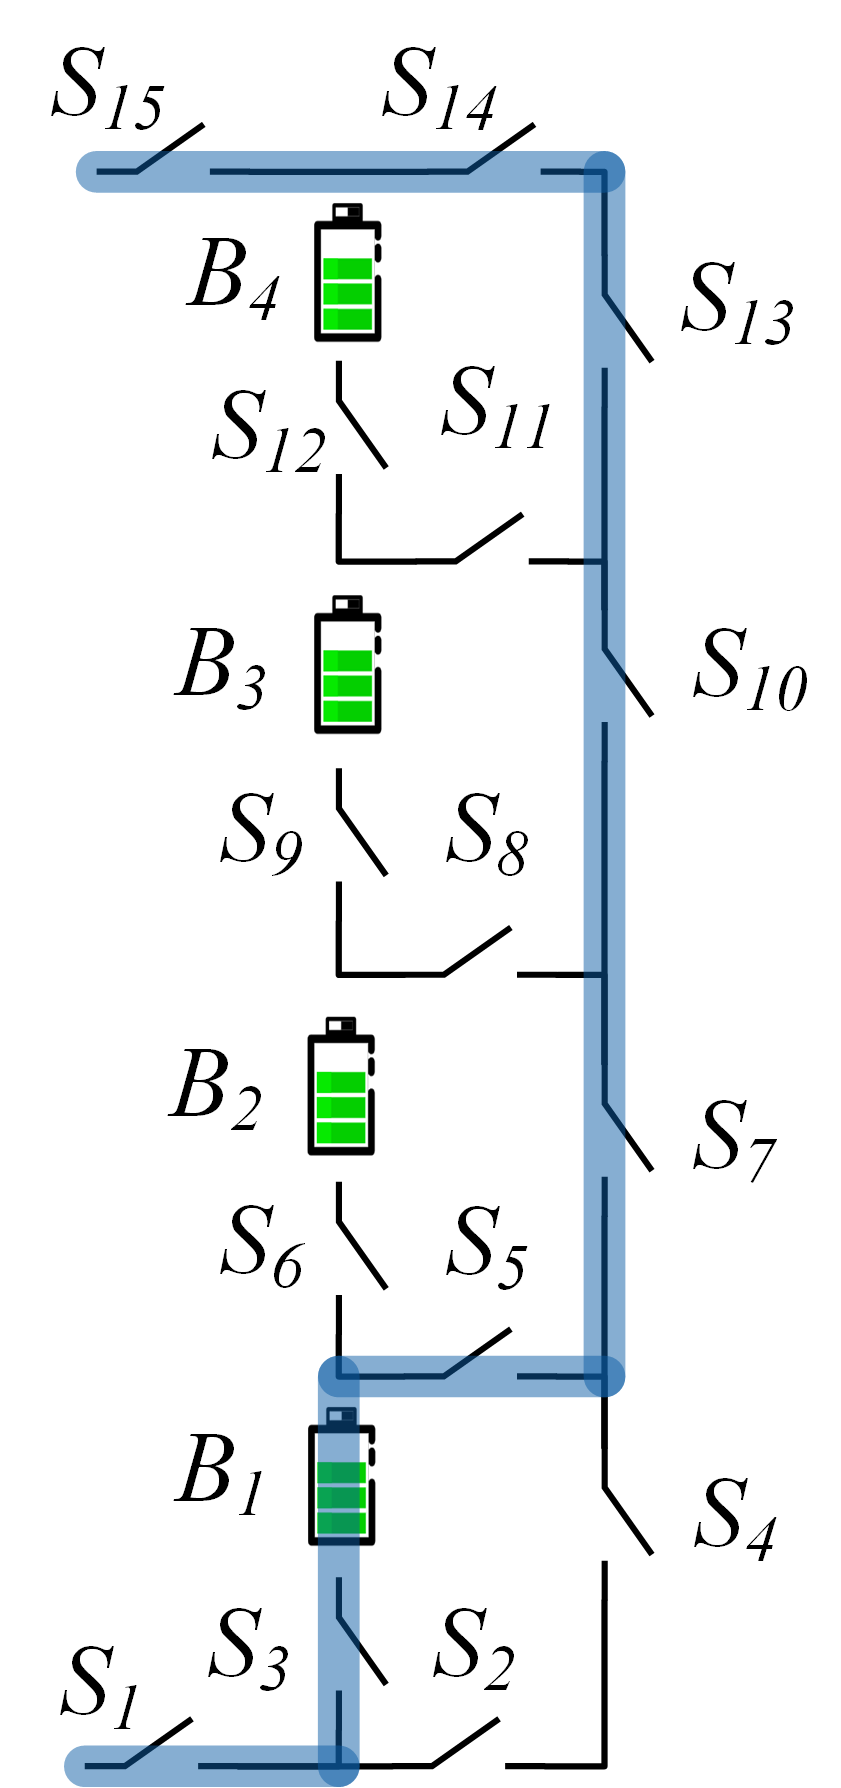
\includegraphics[width=\textwidth]{e4-mac.png}
        \caption{}
        \label{fig:e4-mac}
    \end{subfigure}
    \DIFaddFL{\hspace{0.02\textwidth}
    }\begin{subfigure}[b]{0.4\textwidth}
        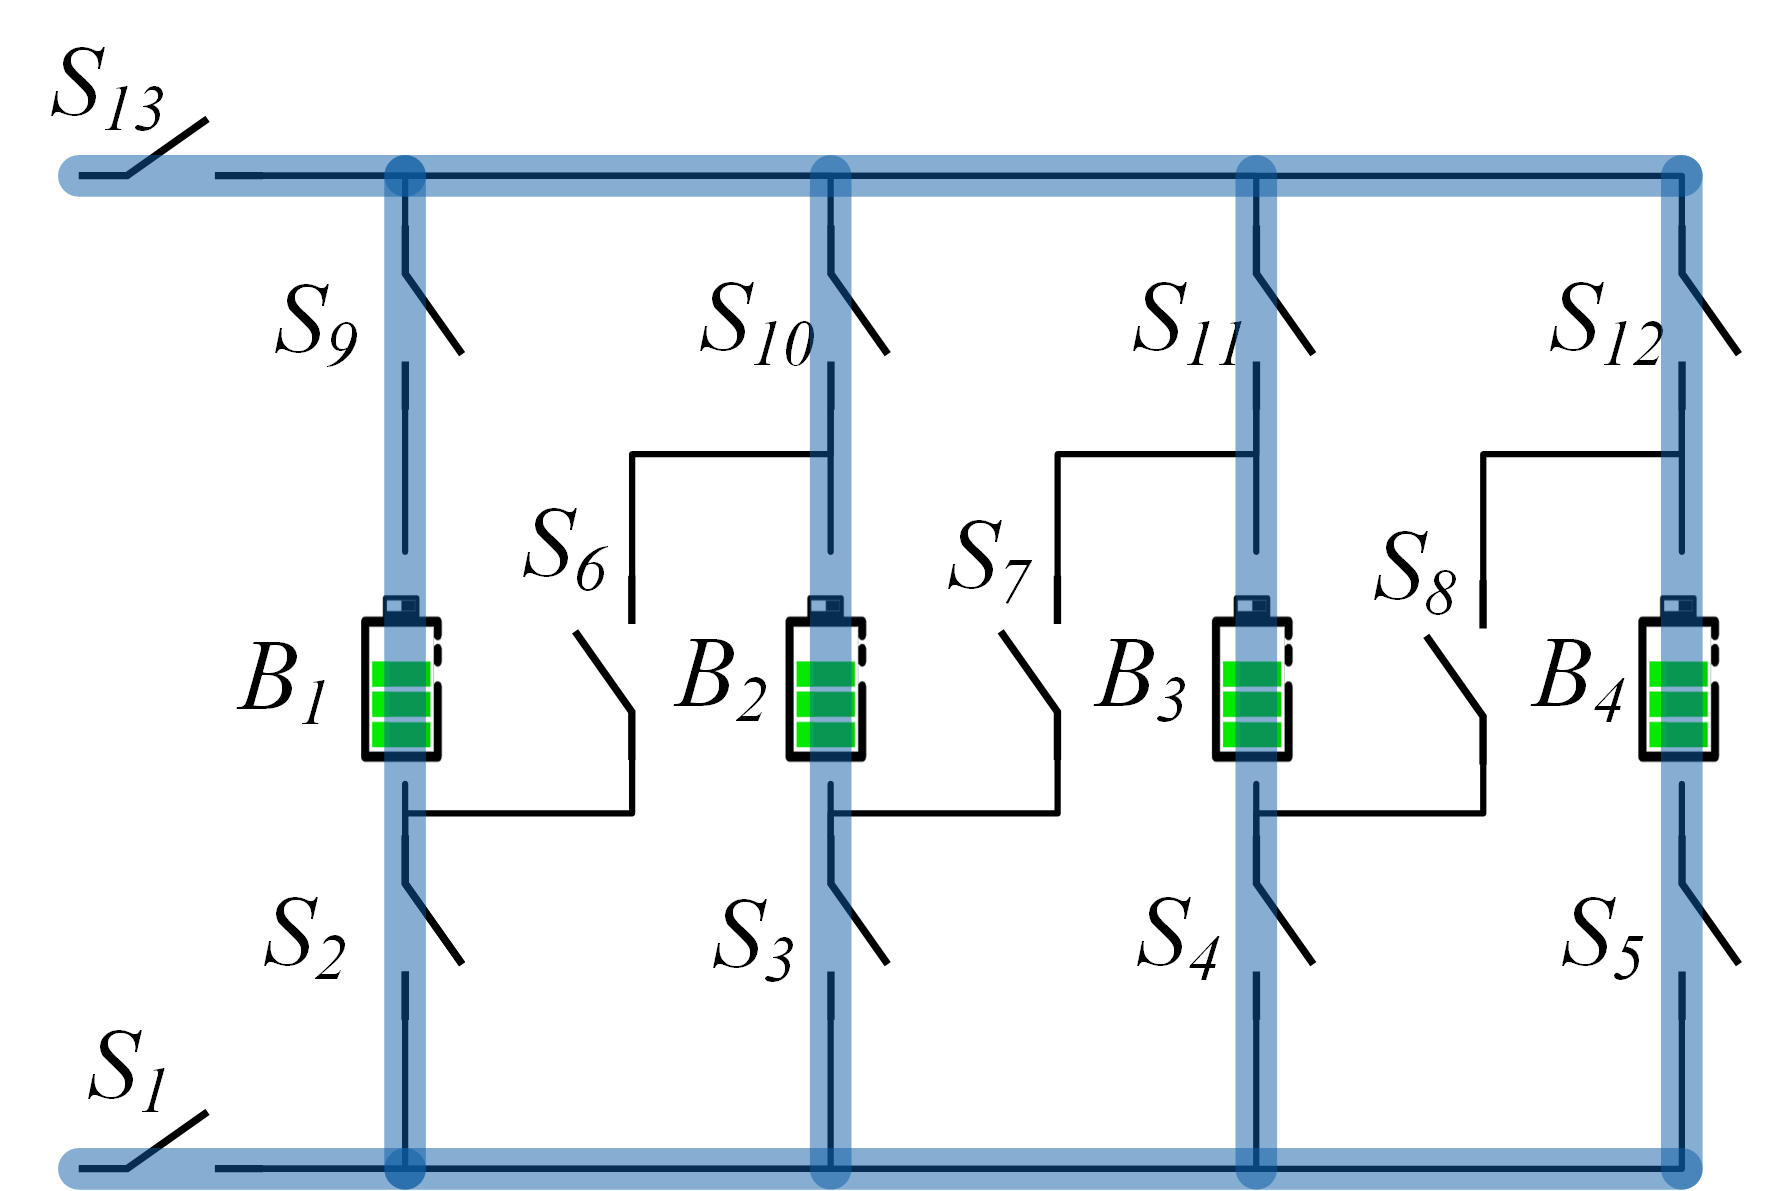
\includegraphics[width=\textwidth]{f4-mac.png}
        \caption{}
        \label{fig:f4-mac}
    \end{subfigure}
    \DIFaddFL{\hspace{0.02\textwidth}
    }\begin{subfigure}[b]{0.31\textwidth}
        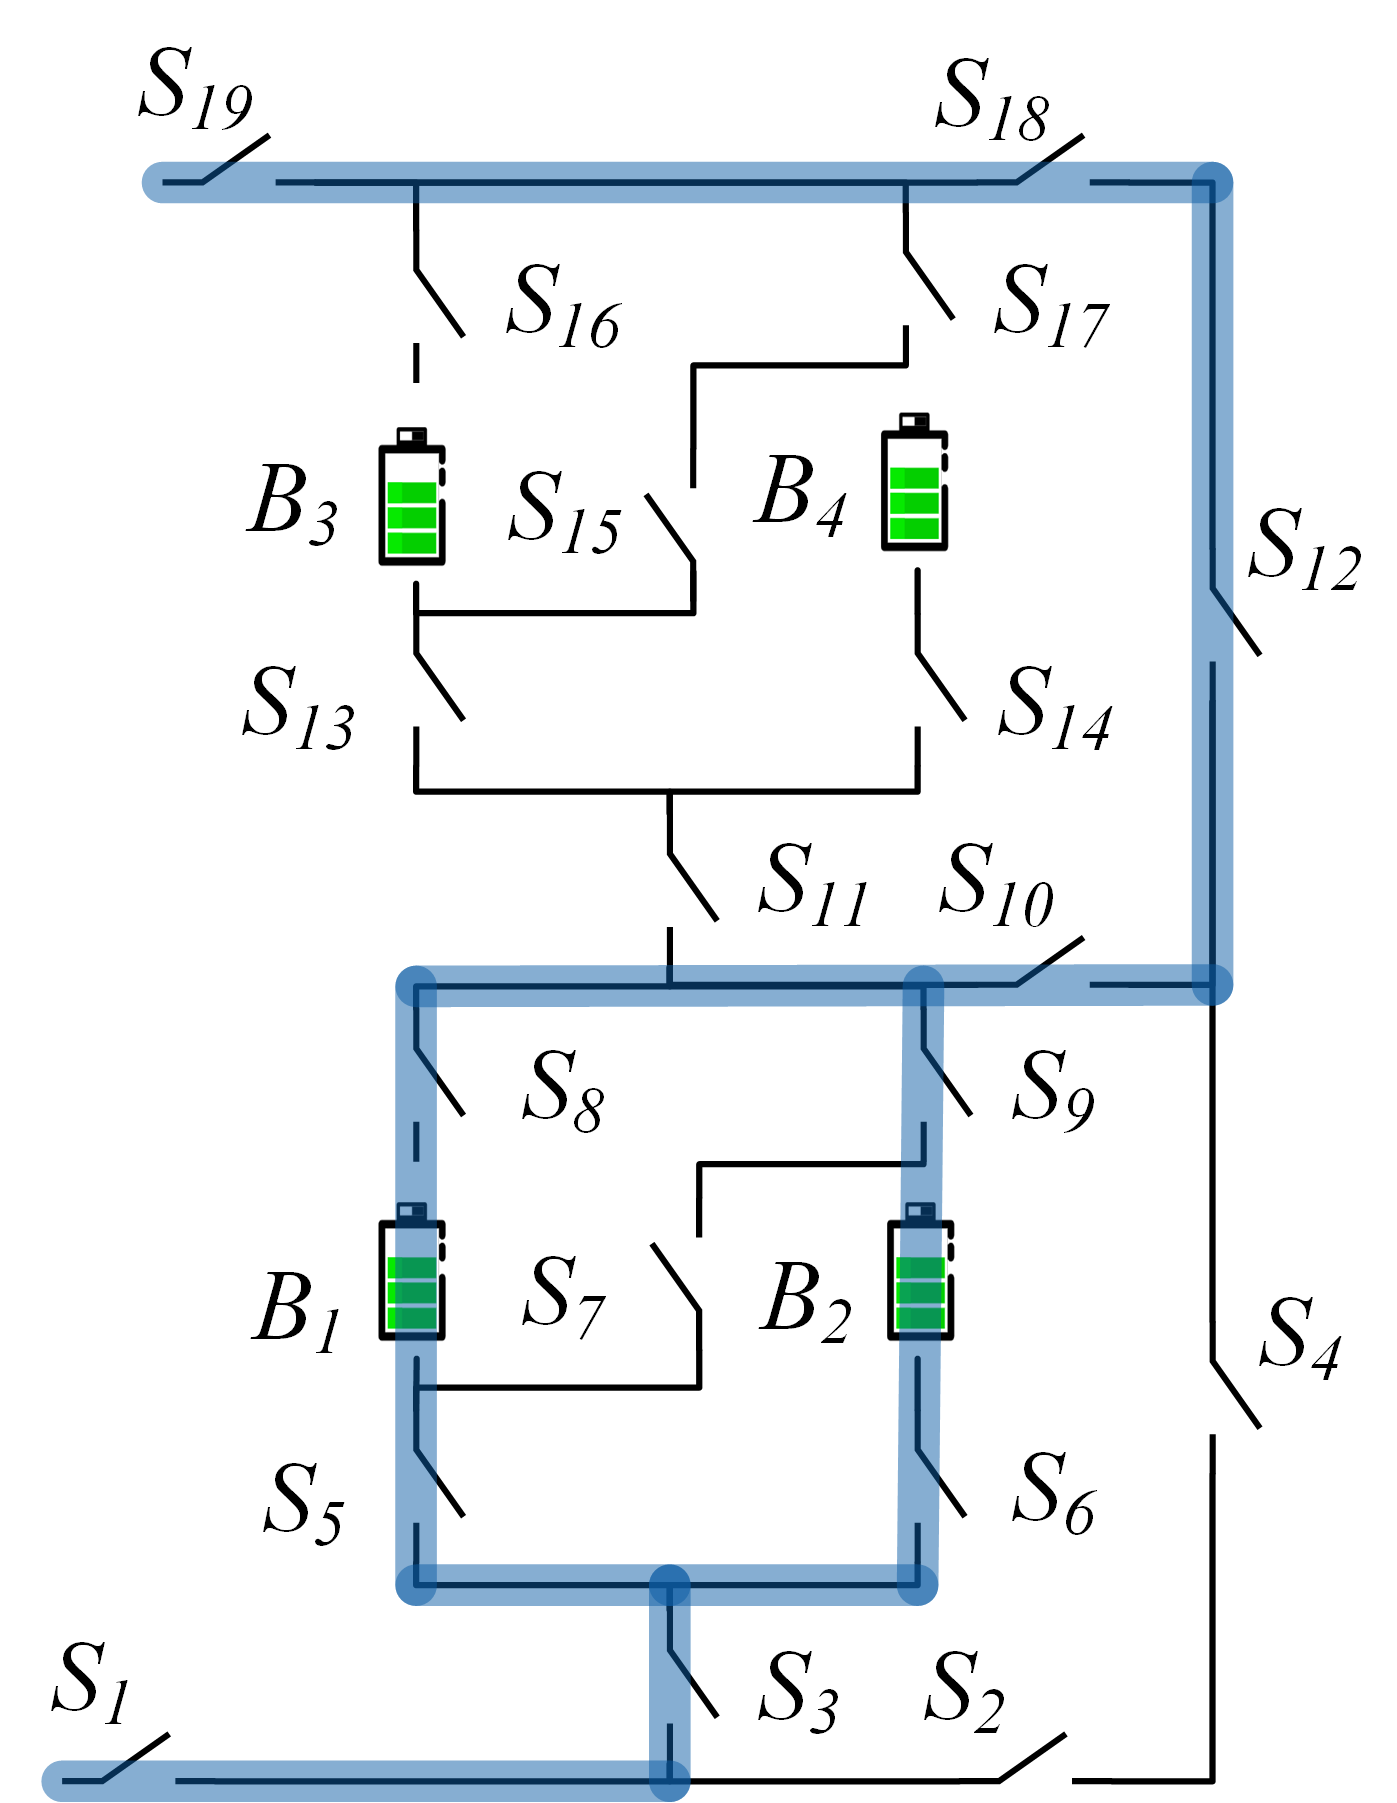
\includegraphics[width=\textwidth]{e2f2-mac.png}
        \caption{}
        \label{fig:e2f2-mac}
    \end{subfigure}
    \caption{\DIFaddFL{The RBS switch-control schemes with the output reaching the MAC.}}
\end{figure}

\begin{figure}[htbp]
    \centering
    \begin{subfigure}[b]{0.32\textwidth}
        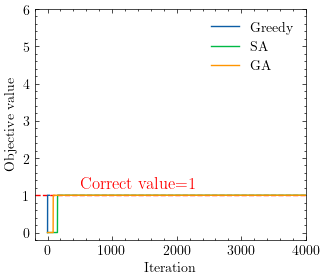
\includegraphics[width=\textwidth]{e4-alg.png}
        \caption{}
        \label{fig:e4-alg}
    \end{subfigure}
    %DIF >  \hspace{0.02\textwidth}
    \begin{subfigure}[b]{0.32\textwidth}
        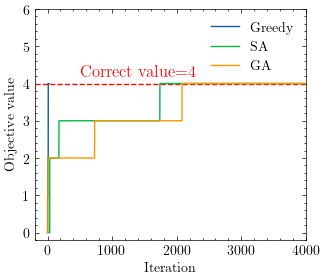
\includegraphics[width=\textwidth]{f4-alg}
        \caption{}
        \label{fig:f4-alg}
    \end{subfigure}
    %DIF >  \hspace{0.02\textwidth}
    \begin{subfigure}[b]{0.32\textwidth}
        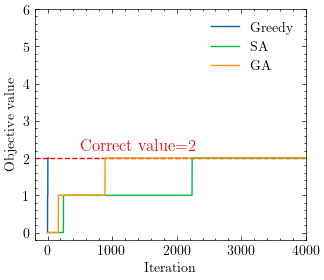
\includegraphics[width=\textwidth]{e2f2-alg}
        \caption{}
        \label{fig:e2f2-alg}
    \end{subfigure}
    \caption{\DIFaddFL{The temporal evolution of the objective values during the iteration process of calculating the RBS structures in (a) Fig. \ref{fig:study-stru-Lawson}, (b) Fig. \ref{fig:study-stru-Visairo}, and (c) Fig. \ref{fig:study-stru-my}}}
\end{figure}

\subsubsection{\DIFadd{Structures with different numbers of batteries}}

\DIFadd{We next examine the RBS configurations depicted in Fig. \ref{fig:study-stru-my}, which consist of two, four, and six batteries.
The }\DIFaddend results for the \DIFdelbegin \DIFdel{three structures under study, with varying numbers of isolated batteries, }\DIFdelend \DIFaddbegin \DIFadd{four-battery configuration }\DIFaddend are presented in Tab. \DIFdelbegin \DIFdel{\ref{tab:isolated_mac}. 
Figs. \ref{fig:my-isolated-1}--\ref{fig:my-isolated-3} illustrate the corresponding }\DIFdelend \DIFaddbegin \DIFadd{\ref{tab:study-results-my} and Figs. \ref{fig:e2f2-mac} and \ref{fig:e2f2-alg}.
The structures and final }\DIFaddend switch-control schemes for the \DIFdelbegin \DIFdel{new structureproposed in this paper under different conditions of isolated batteries}\DIFdelend \DIFaddbegin \DIFadd{two-battery and six-battery systems are illustrated in Figs. \ref{fig:e2f1-mac} and \ref{fig:e2f3-mac}, respectively.
Furthermore, the temporal evolutions of the objective values throughout the iteration process are shown in Figs. \ref{fig:e2f1-alg} and \ref{fig:e2f3-alg}, respectively.
The proposed greedy algorithm still converges the fastest and achieves the correct MAC. 
The SA algorithm fails to obtain the correct MAC within the given number of iteration steps in the case of the six-battery RBS structure}\DIFaddend . 

\DIFdelbegin %DIFDELCMD < \begin{table}[htbp]
%DIFDELCMD <     %%%
\DIFdelendFL \DIFaddbeginFL \begin{figure}[htbp]
    \DIFaddendFL \centering
    \DIFdelbeginFL %DIFDELCMD < \caption{%
{%DIFAUXCMD
\DIFdelFL{Variation of MAC with the number of isolated batteries for different RBS structures, including the structure proposed by Lawson et al., Visairo et al., and the structure proposed in this paper.
      }}
      %DIFAUXCMD
%DIFDELCMD < \label{tab:isolated_mac}
%DIFDELCMD <       \begin{tabular}{cccc}
%DIFDELCMD <       \toprule
%DIFDELCMD <       \multirow{2}[4]{*}{Number of isolated batteries} & \multicolumn{3}{c}{$\eta$ of RBS structure} \\
%DIFDELCMD <   \cmidrule{2-4}          & %%%
\DIFdelFL{This paper  }%DIFDELCMD < & %%%
\DIFdelFL{Visairo  }%DIFDELCMD < & %%%
\DIFdelFL{Lawson  }%DIFDELCMD < \\
%DIFDELCMD <       \midrule
%DIFDELCMD <       %%%
\DIFdelFL{0     }%DIFDELCMD < & %%%
\DIFdelendFL \DIFaddbeginFL \begin{subfigure}[b]{0.27\textwidth}
        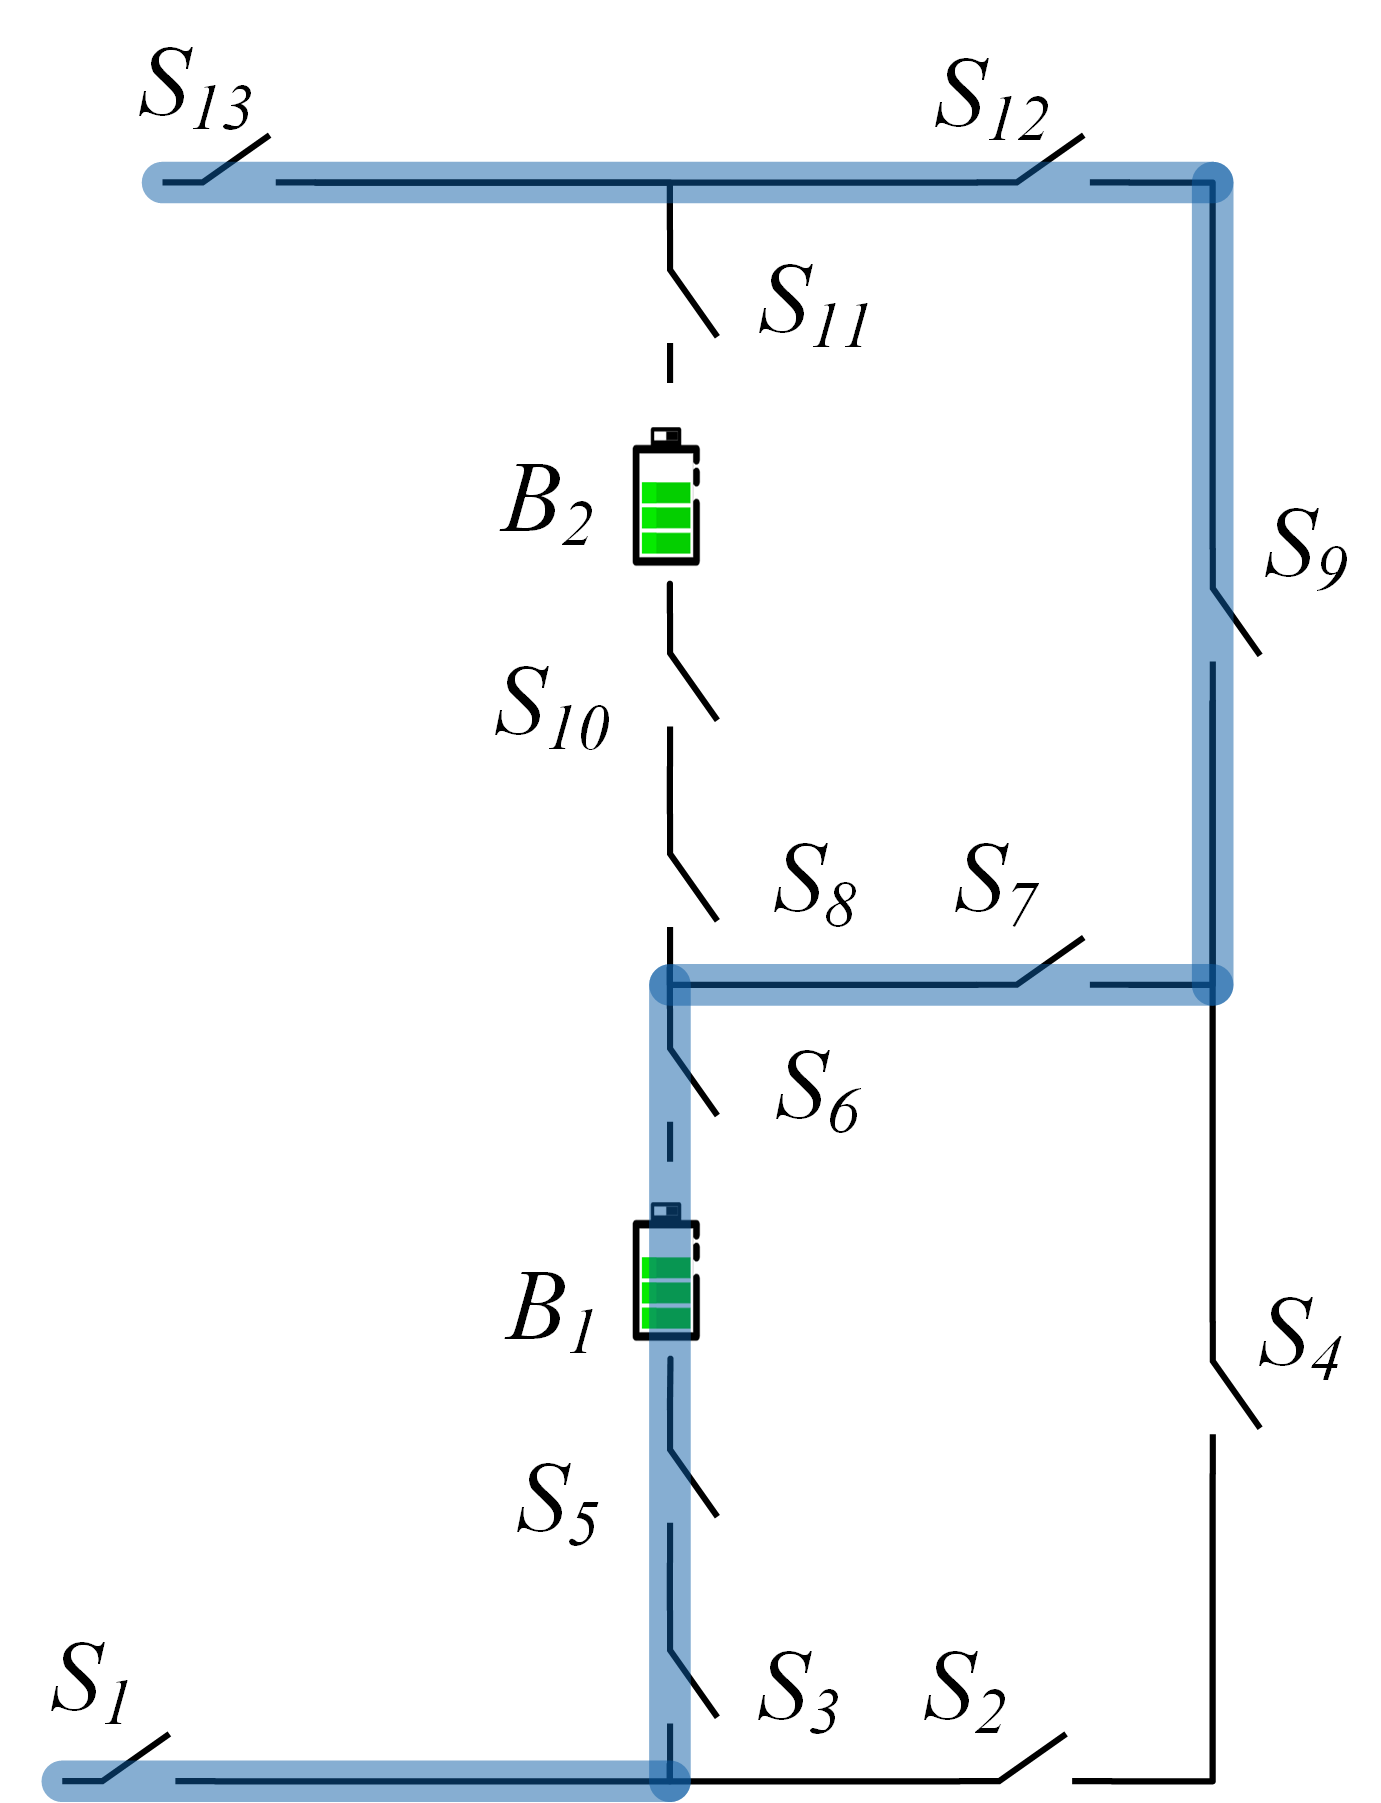
\includegraphics[width=\textwidth]{e2f1-mac.png}
        \caption{}
        \label{fig:e2f1-mac}
    \end{subfigure}
    \DIFaddFL{\hspace{0.02\textwidth}
    }\begin{subfigure}[b]{0.31\textwidth}
        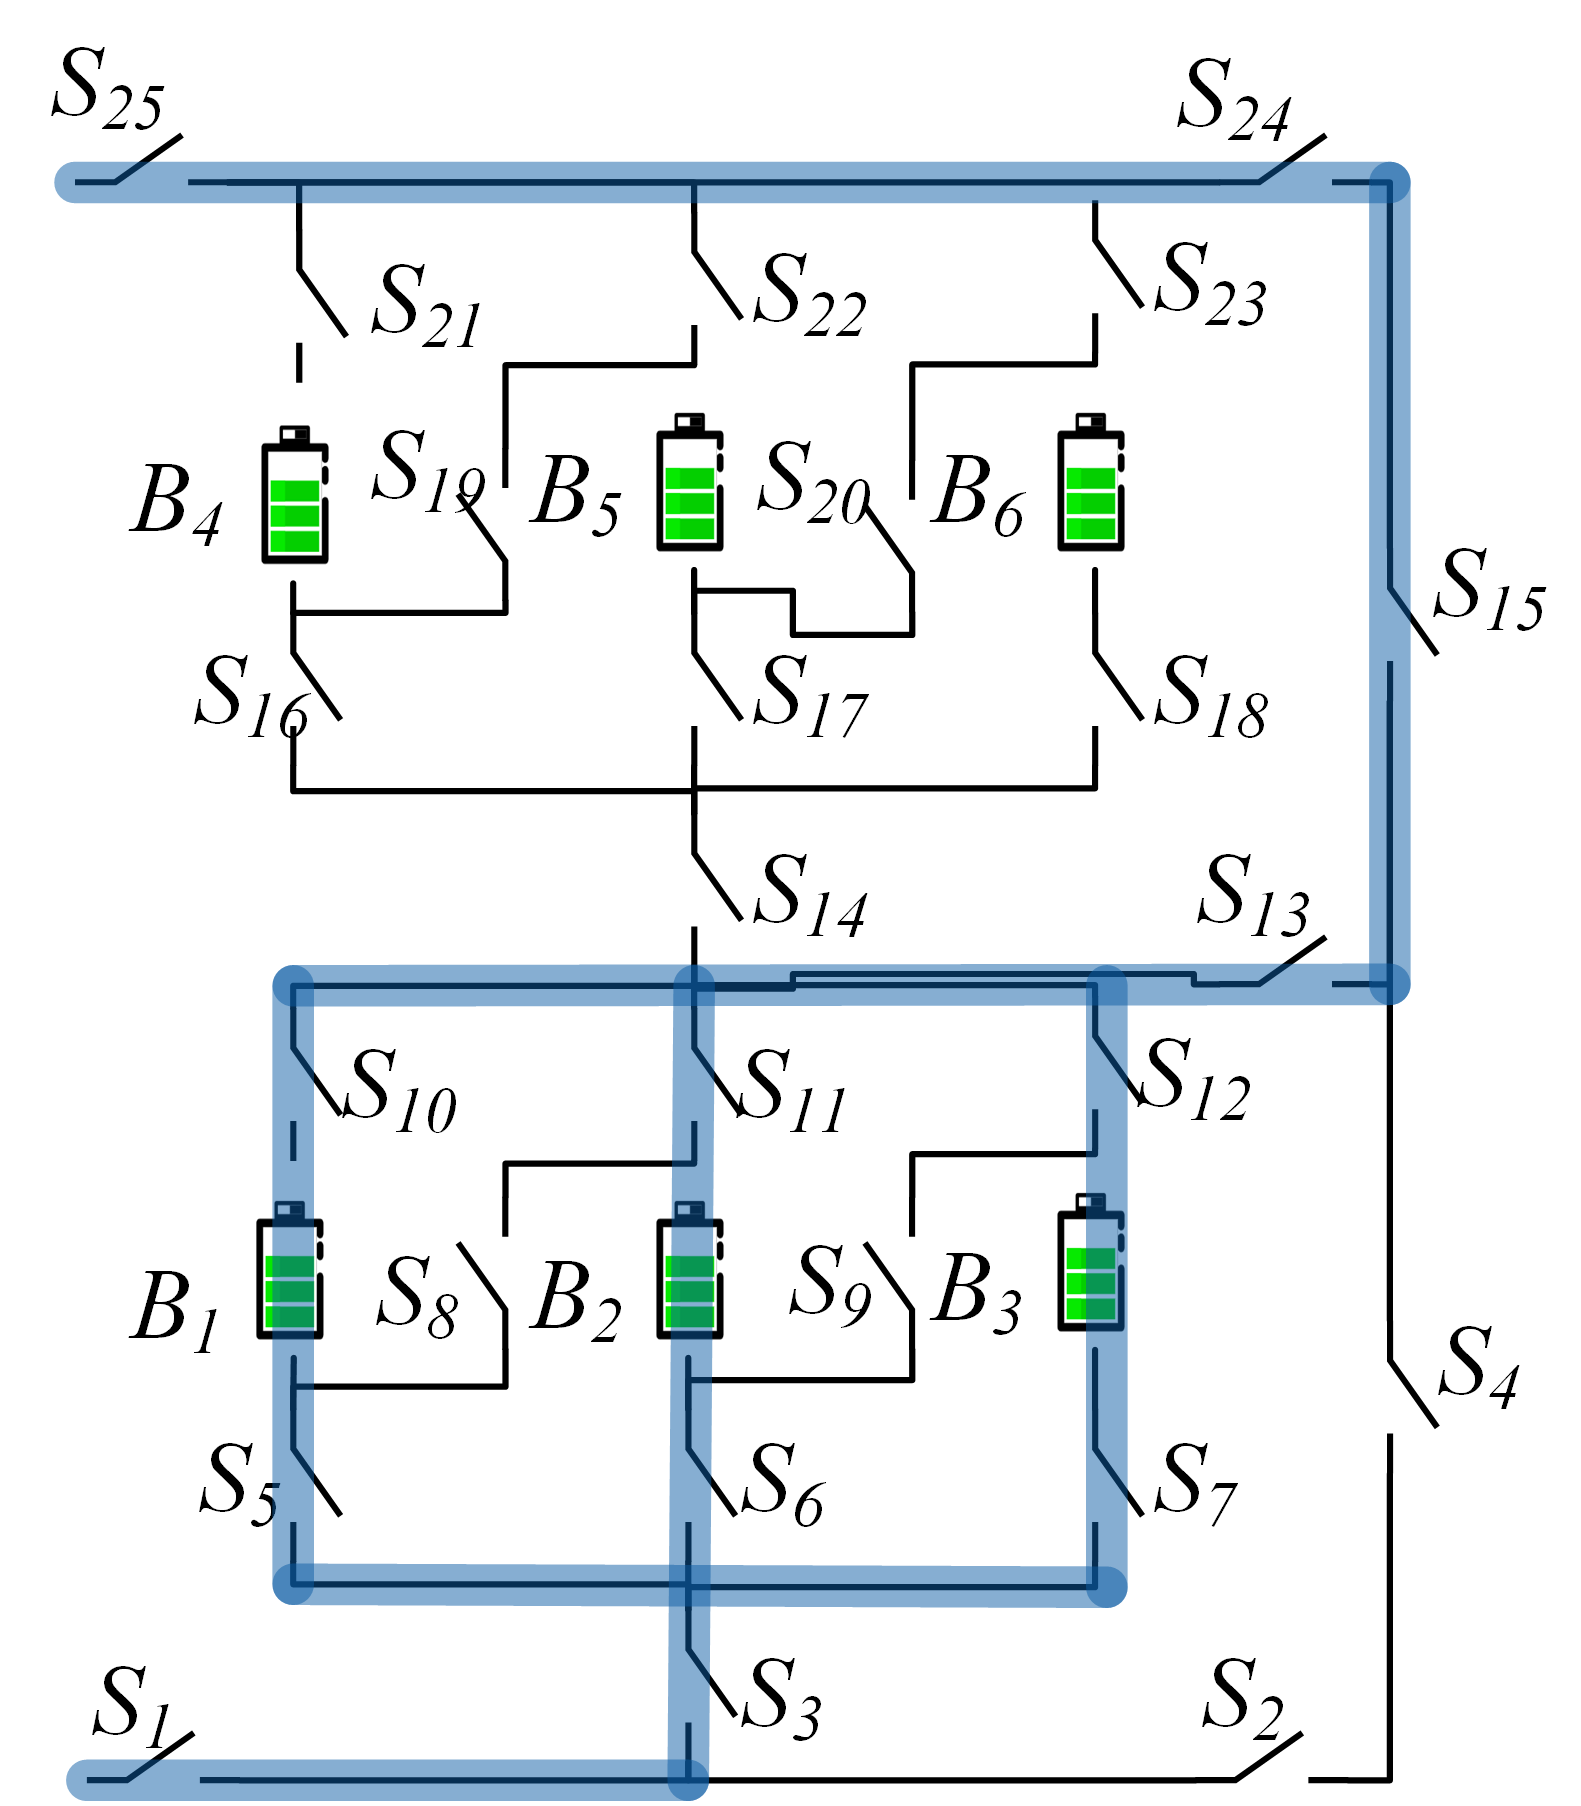
\includegraphics[width=\textwidth]{e2f3-mac.png}
        \caption{}
        \label{fig:e2f3-mac}
    \end{subfigure}
    \caption{\DIFaddFL{The (a) two-battery and (b) six-battery RBS switch-control schemes with the output reaching the MAC.}}
\end{figure}

\begin{figure}[htbp]
    \centering
    \begin{subfigure}[b]{0.34\textwidth}
        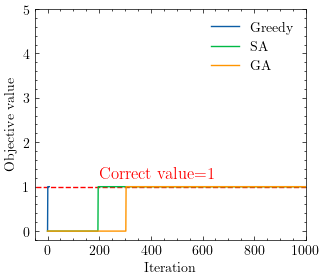
\includegraphics[width=\textwidth]{e2f1-alg.png}
        \caption{}
        \label{fig:e2f1-alg}
    \end{subfigure}
    \DIFaddFL{\hspace{0.02\textwidth}
    }\begin{subfigure}[b]{0.33\textwidth}
        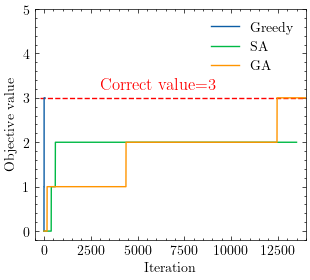
\includegraphics[width=\textwidth]{e2f3-alg.png}
        \caption{}
        \label{fig:e2f3-alg}
    \end{subfigure}
    \caption{\DIFaddFL{The temporal variation of the objective values during the iteration process of calculating the RBS structures in (a) Fig. \ref{fig:e2f1-mac} and (b) Fig. \ref{fig:e2f3-mac}.}}
\end{figure}

\subsubsection{\DIFaddFL{Random isolated batteries}}

\DIFaddFL{To assess the effectiveness of the proposed algorithm in the case of unhealthy batteries, the RBS with random isolated batteries is also taken into account and computed. 
In the case of the four-battery RBS structure depicted in Fig. \ref{fig:study-stru-my}, there are four possible scenarios for isolated batteries: (a) a single unhealthy battery, (b) two unhealthy batteries located in different substructures, (c) two unhealthy batteries located in the same substructure, and (d) three unhealthy batteries. 
The resulting MAC ($\eta$) values for these four scenarios are }\DIFaddendFL 2\DIFdelbeginFL %DIFDELCMD < & %%%
\DIFdelFL{4     }%DIFDELCMD < & %%%
\DIFdelFL{1 }%DIFDELCMD < \\
%DIFDELCMD <       %%%
\DIFdelFL{1     }%DIFDELCMD < & %%%
\DIFdelendFL \DIFaddbeginFL \DIFaddFL{, }\DIFaddendFL 2\DIFdelbeginFL %DIFDELCMD < & %%%
\DIFdelFL{3     }%DIFDELCMD < & %%%
\DIFdelendFL \DIFaddbeginFL \DIFaddFL{, }\DIFaddendFL 1\DIFdelbeginFL %DIFDELCMD < \\
%DIFDELCMD <       %%%
\DIFdelFL{2     }%DIFDELCMD < & %%%
\DIFdelFL{2$^{\mathrm{a}}$ or }\DIFdelendFL \DIFaddbeginFL \DIFaddFL{, and }\DIFaddendFL 1\DIFdelbeginFL \DIFdelFL{$^{\mathrm{b}}$ }%DIFDELCMD < & %%%
\DIFdelFL{2     }%DIFDELCMD < & %%%
\DIFdelFL{1 }%DIFDELCMD < \\
%DIFDELCMD <       %%%
\DIFdelFL{3     }%DIFDELCMD < & %%%
\DIFdelFL{1     }%DIFDELCMD < & %%%
\DIFdelFL{1     }%DIFDELCMD < & %%%
\DIFdelFL{1 }%DIFDELCMD < \\
%DIFDELCMD <       \bottomrule
%DIFDELCMD <       \end{tabular}
%DIFDELCMD <       \\
%DIFDELCMD <       \footnotesize{$^{\mathrm{a}}$ Isolate two batteries within the same substructure, as shown in Fig. \ref{fig:my-isolated-2b}.}\\
%DIFDELCMD <       \footnotesize{$^{\mathrm{b}}$ Isolate one battery in each of the two substructures, as shown in Fig. \ref{fig:my-isolated-2w}.}
%DIFDELCMD <   \end{table}
%DIFDELCMD <   %%%
\DIFdelend \DIFaddbegin \DIFadd{, respectively.
Furthermore, the corresponding switch-control schemes for the four scenarios are illustrated in Figs \ref{fig:my-isolated-1}--\ref{fig:my-isolated-3}.
}\DIFaddend 

\begin{figure}[htbp]
    \centering
    \begin{subfigure}[b]{0.31\textwidth}
        \DIFdelbeginFL %DIFDELCMD < 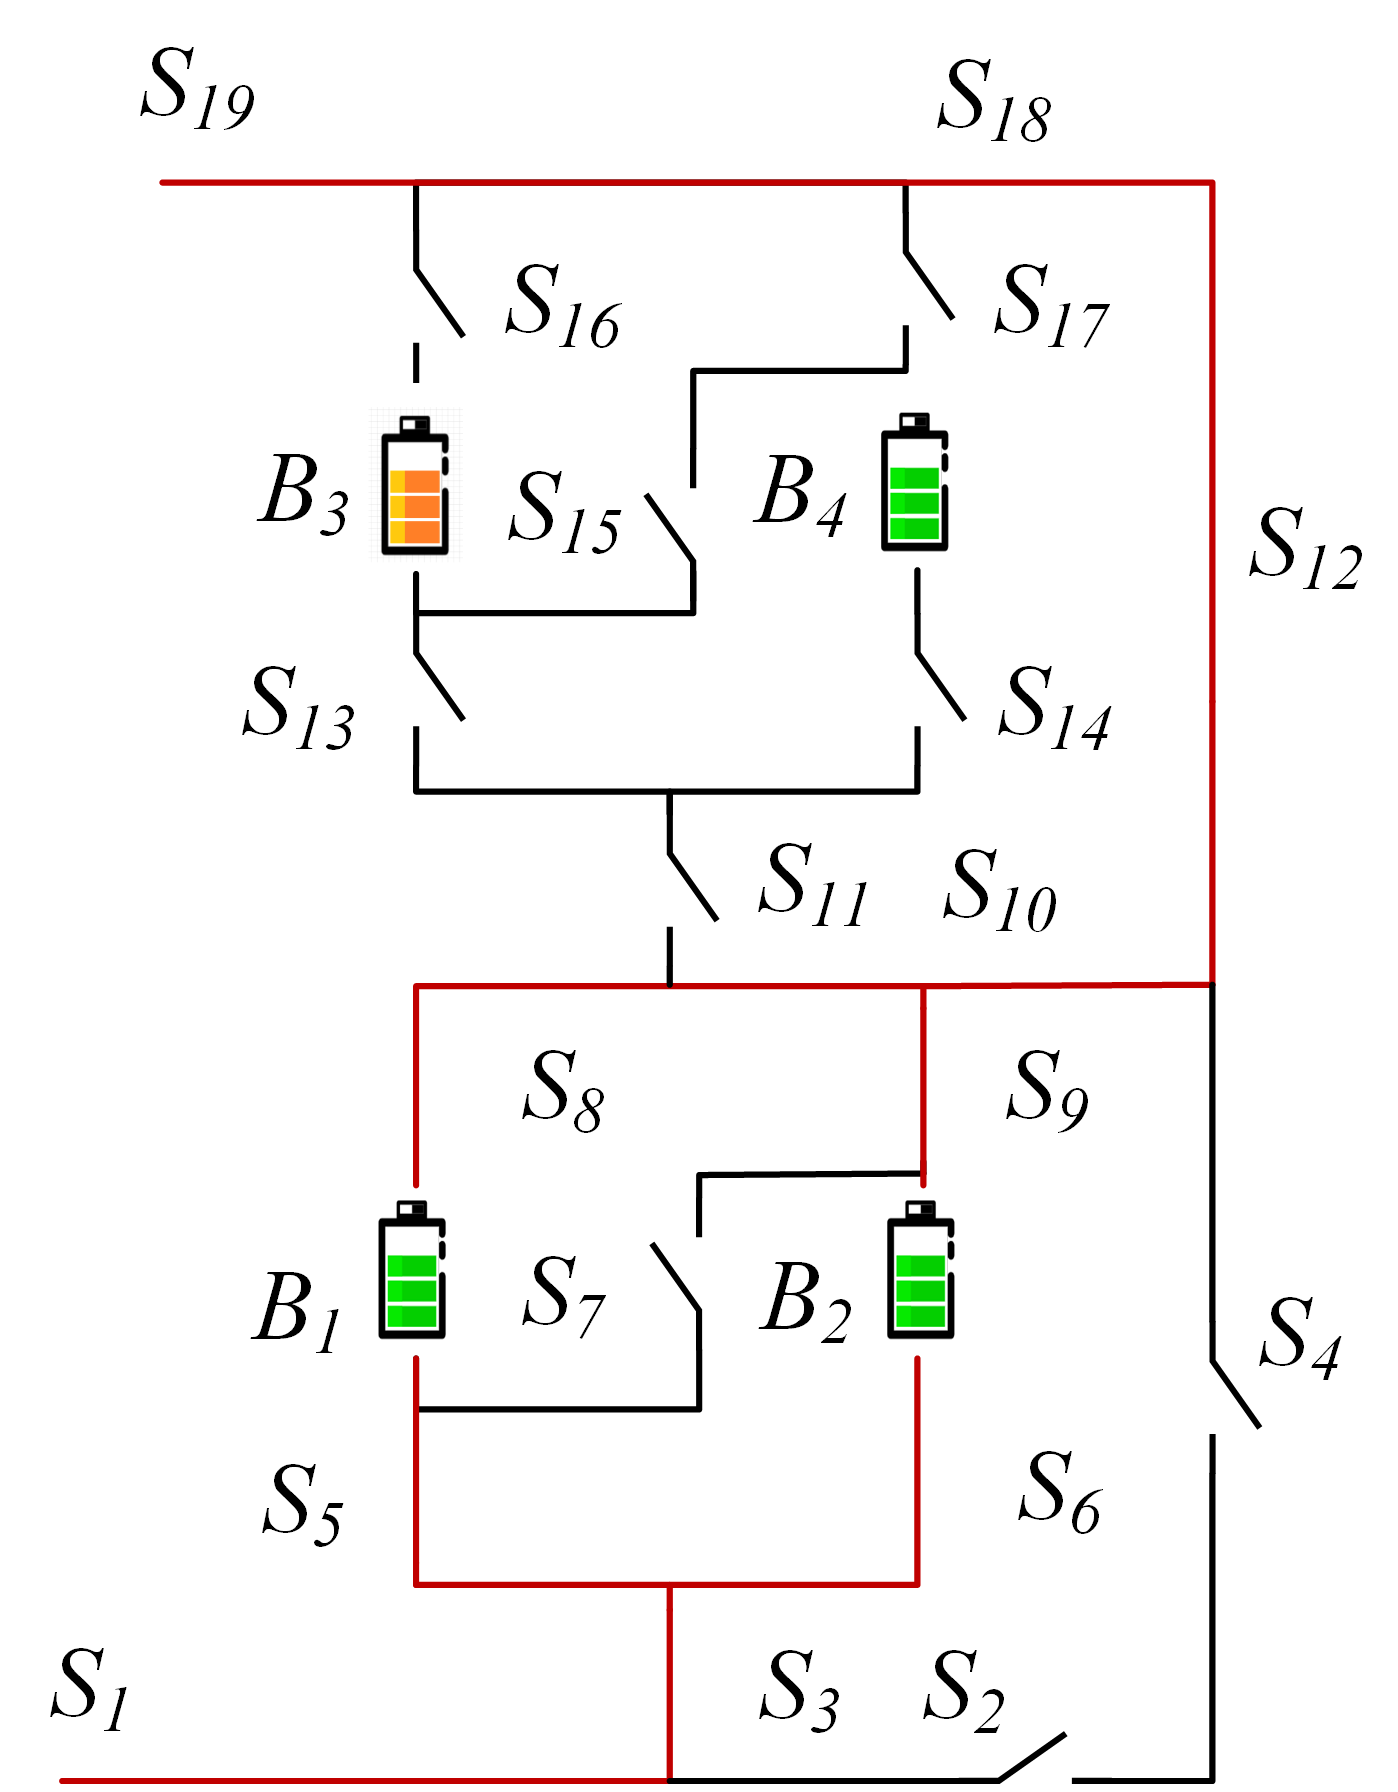
\includegraphics[width=\textwidth]{my-isolated-1.png}
%DIFDELCMD <           %%%
\DIFdelendFL \DIFaddbeginFL 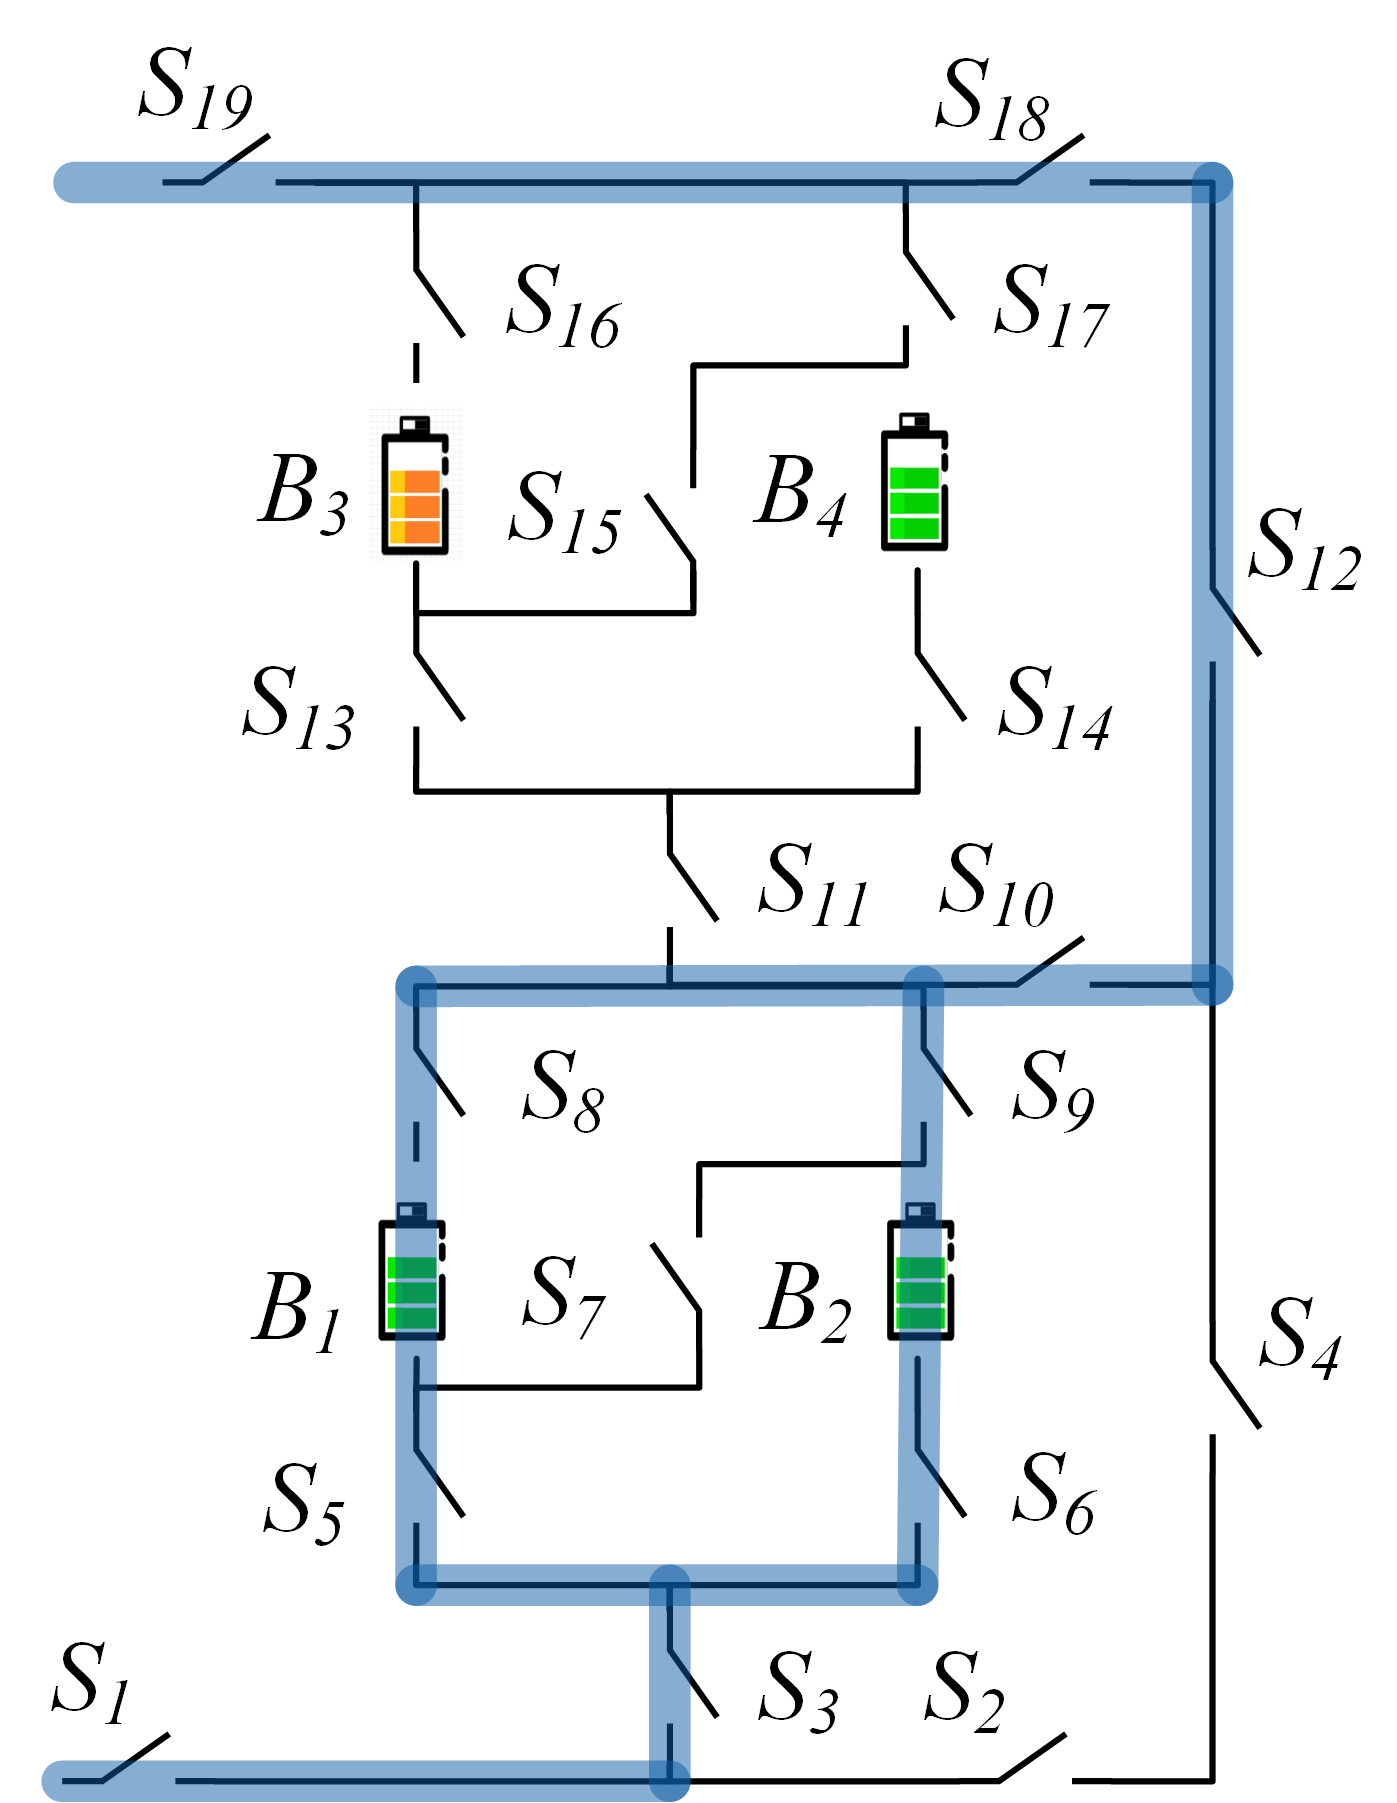
\includegraphics[width=\textwidth]{e2f2-isolate-1.png}
        \DIFaddendFL \caption{}
        \label{fig:my-isolated-1}
    \end{subfigure}
    \hspace{0.02\textwidth}
    \begin{subfigure}[b]{0.31\textwidth}
        \DIFdelbeginFL %DIFDELCMD < 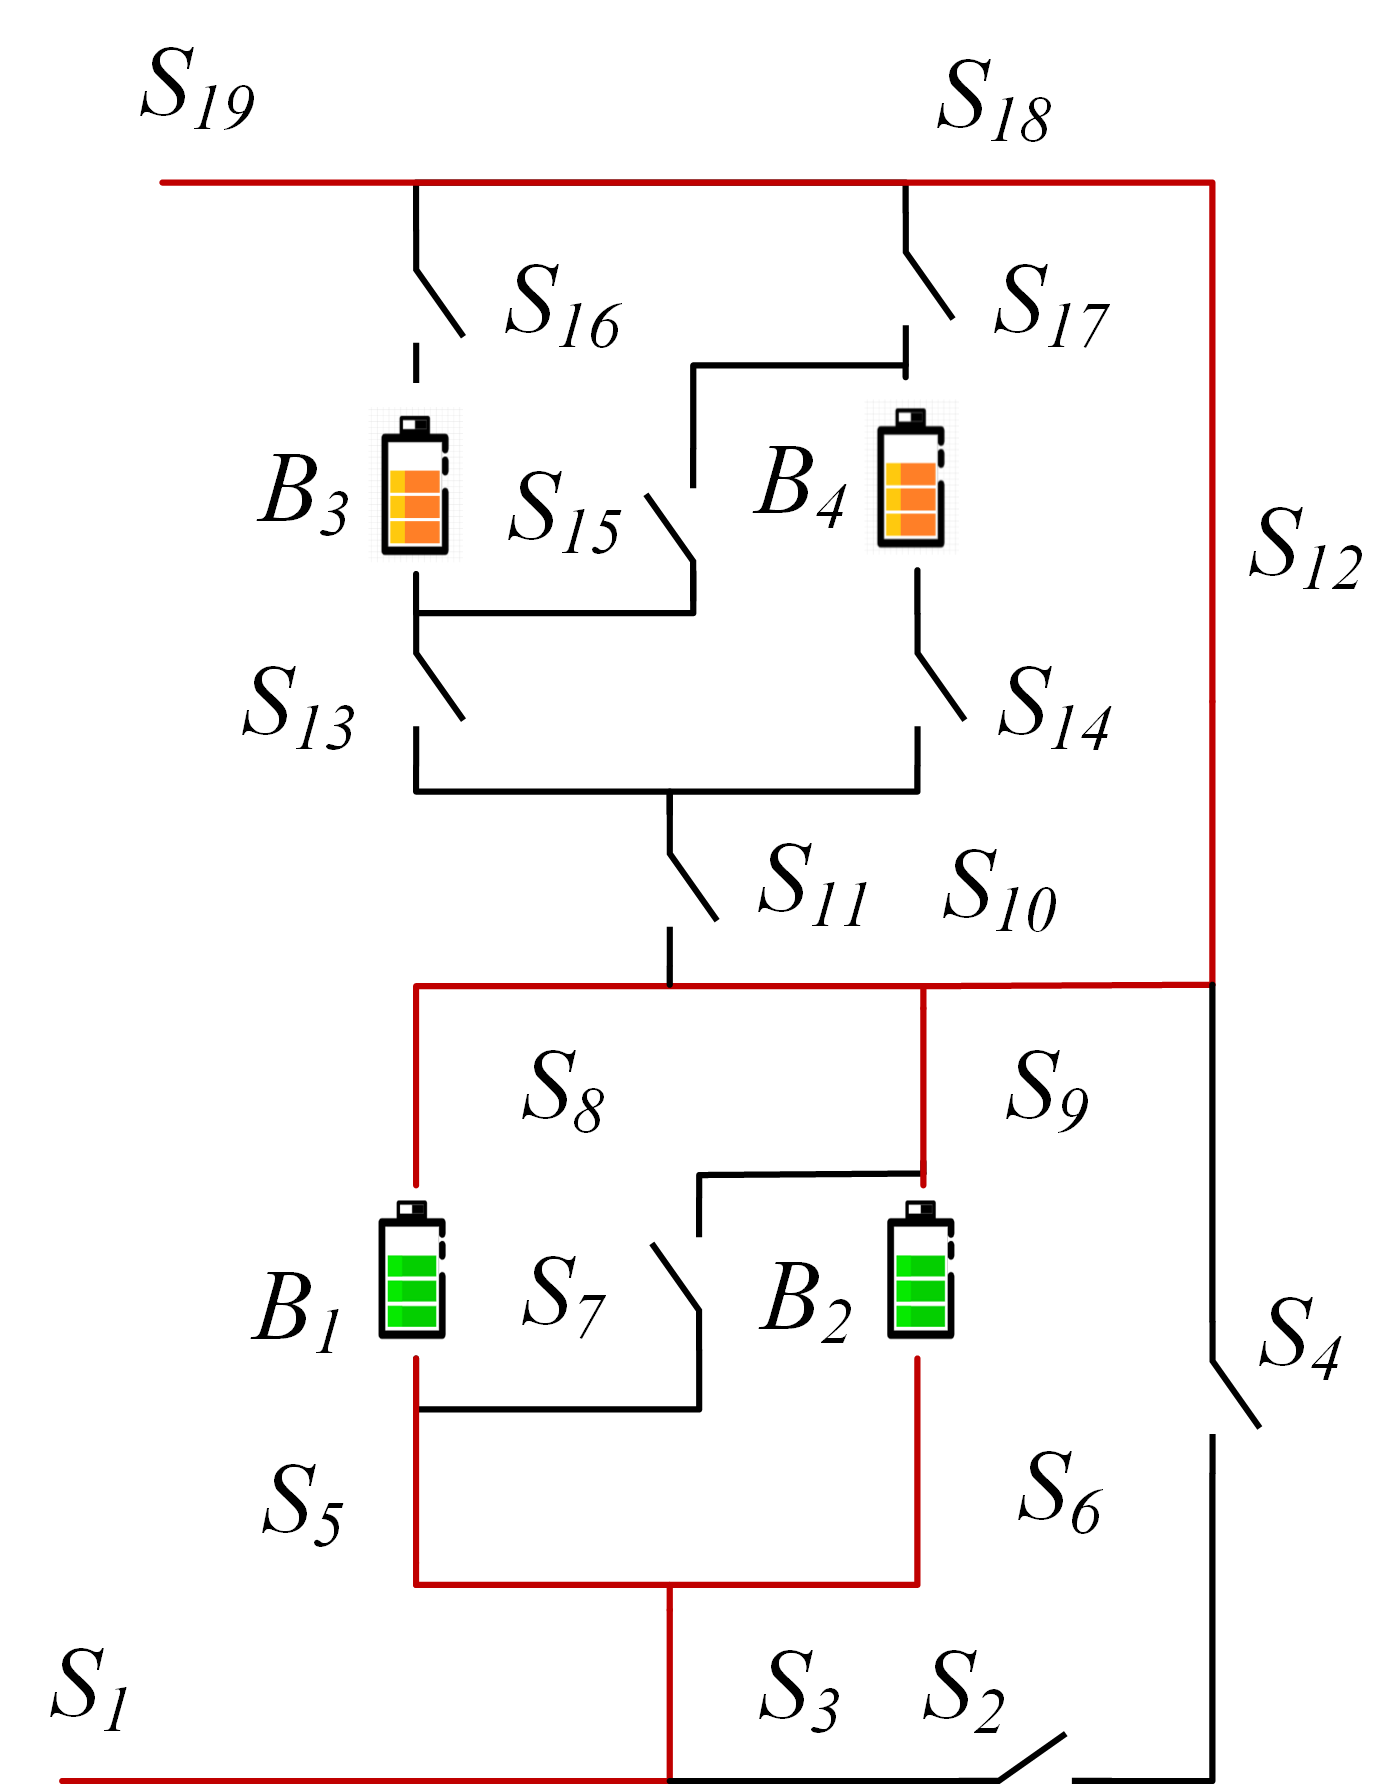
\includegraphics[width=\textwidth]{my-isolated-2b.png}
%DIFDELCMD <           %%%
\DIFdelendFL \DIFaddbeginFL 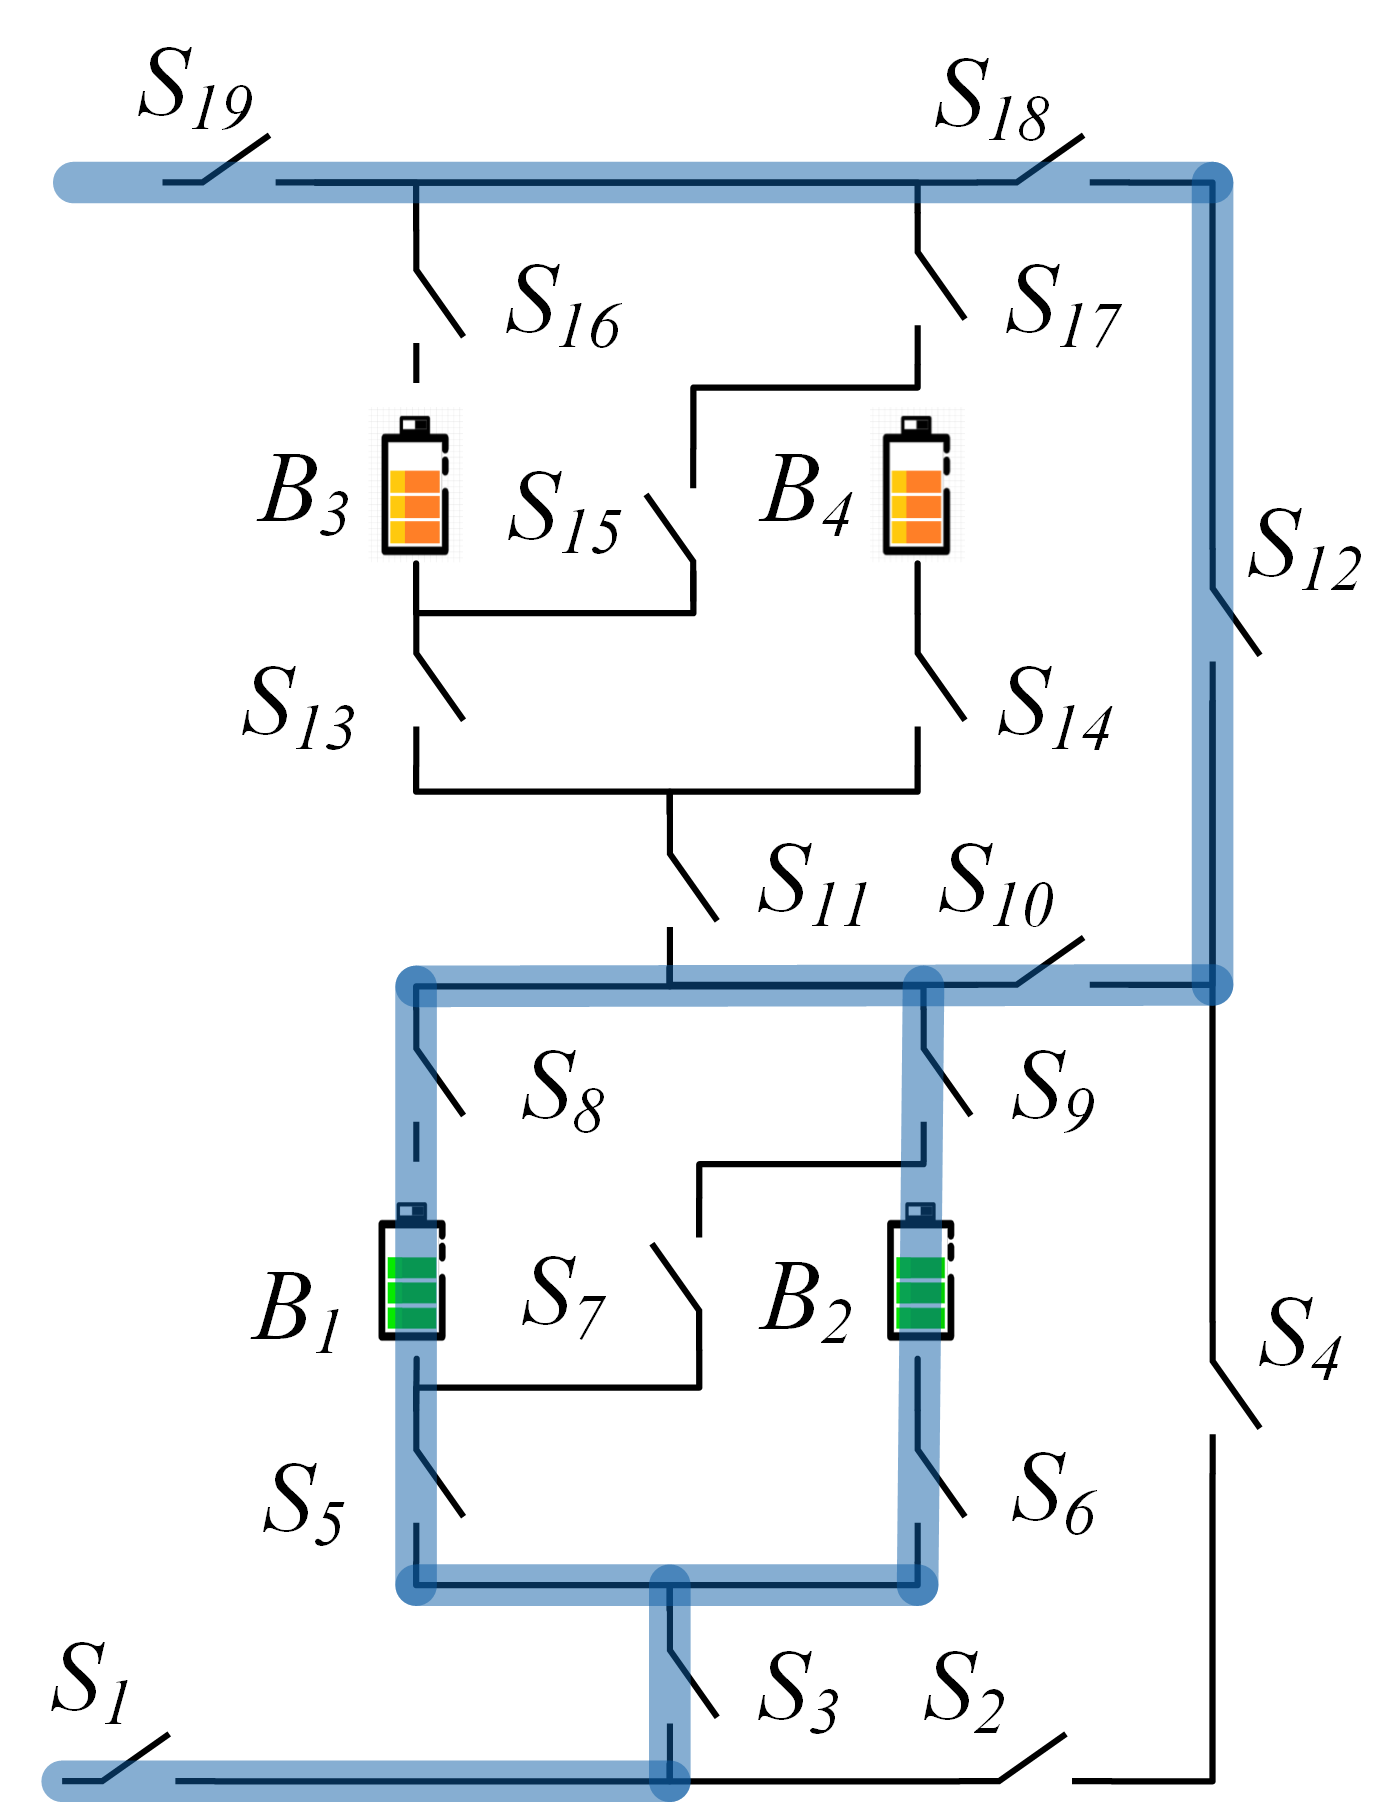
\includegraphics[width=\textwidth]{e2f2-isolate-2b.png}
        \DIFaddendFL \caption{}
        \label{fig:my-isolated-2b}
    \end{subfigure}
    \\
    \begin{subfigure}[b]{0.31\textwidth}
        \DIFdelbeginFL %DIFDELCMD < 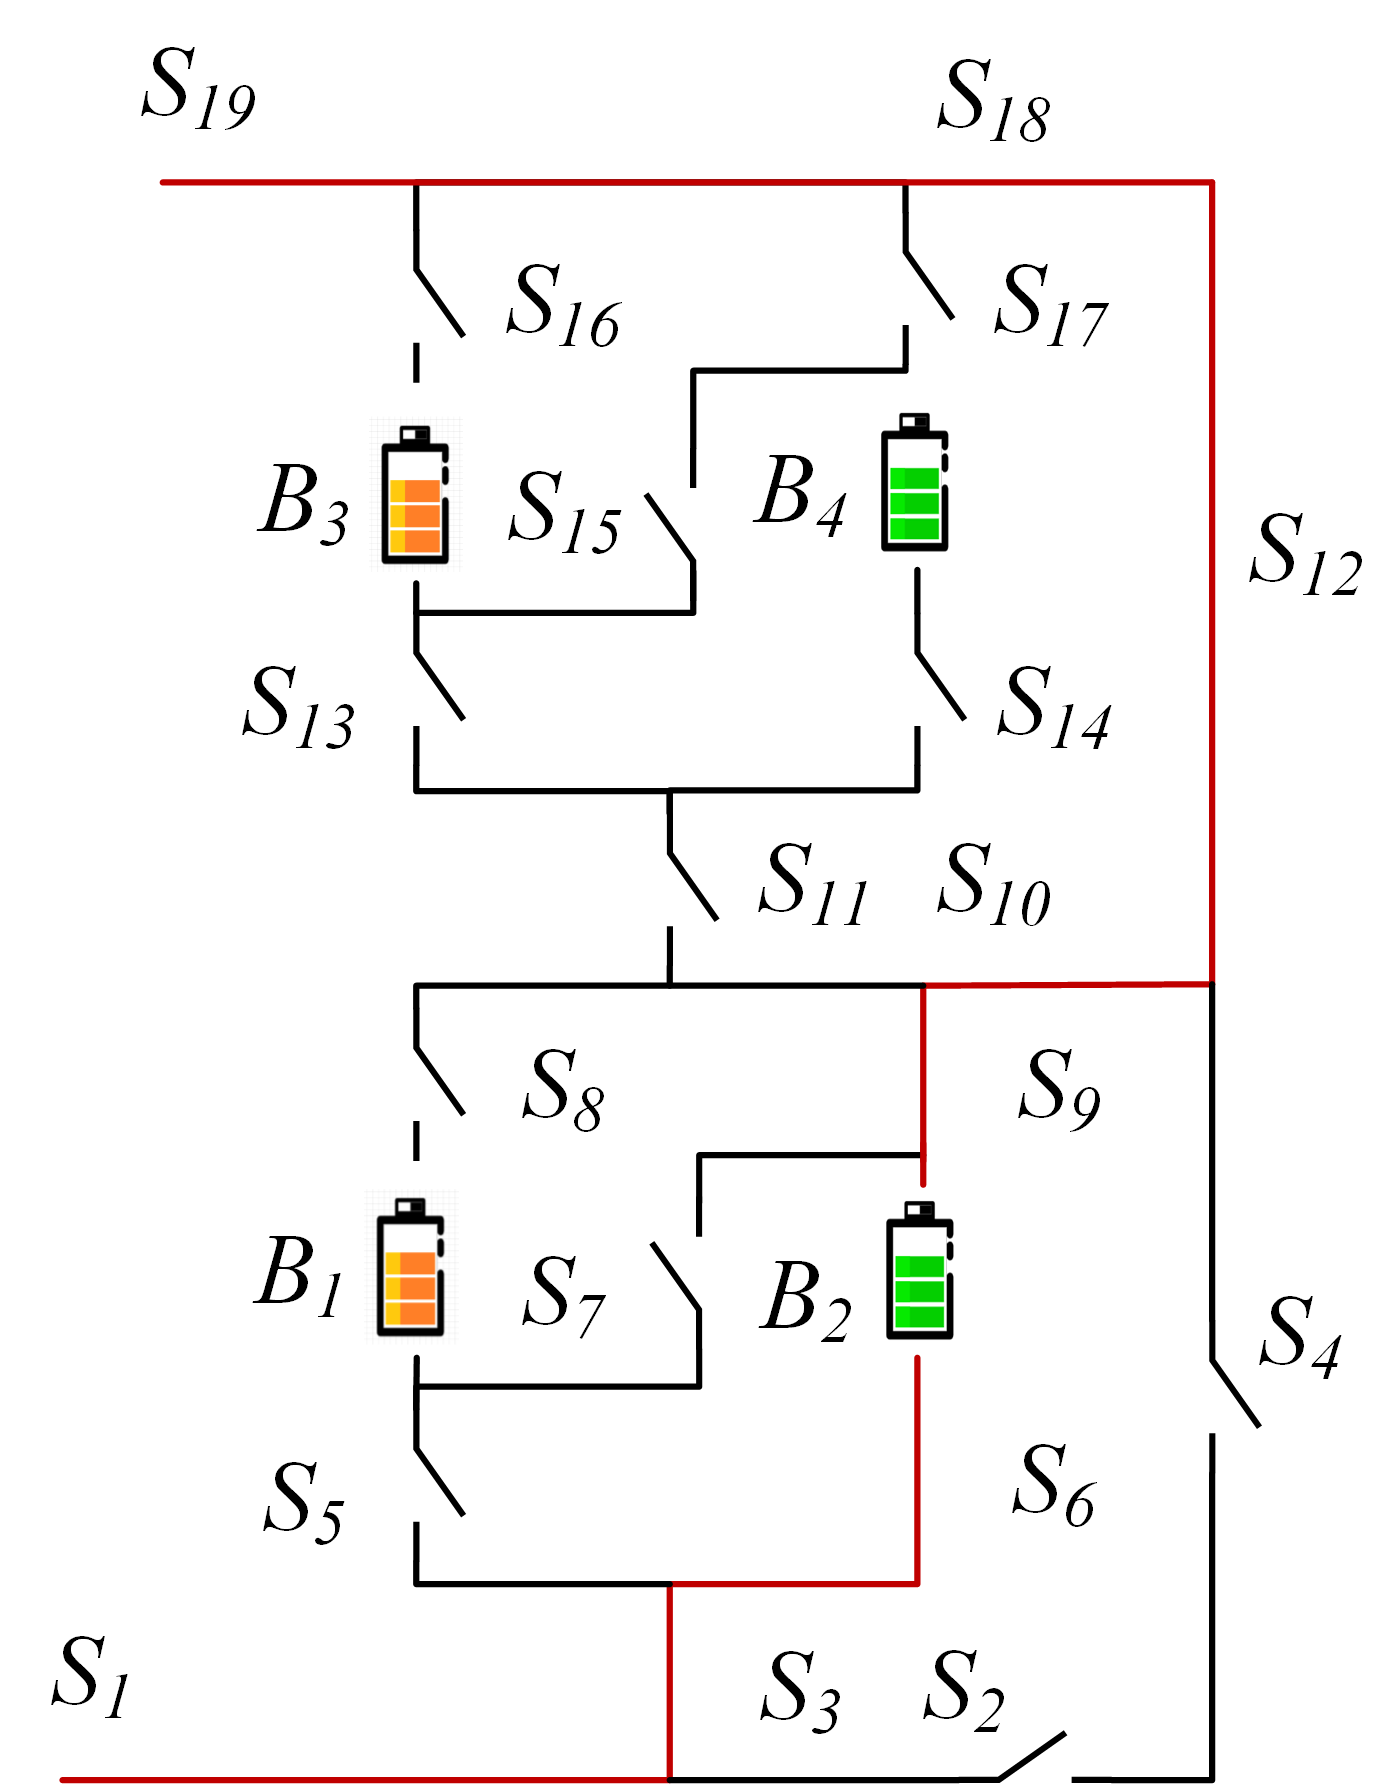
\includegraphics[width=\textwidth]{my-isolated-2w.png}
%DIFDELCMD <           %%%
\DIFdelendFL \DIFaddbeginFL 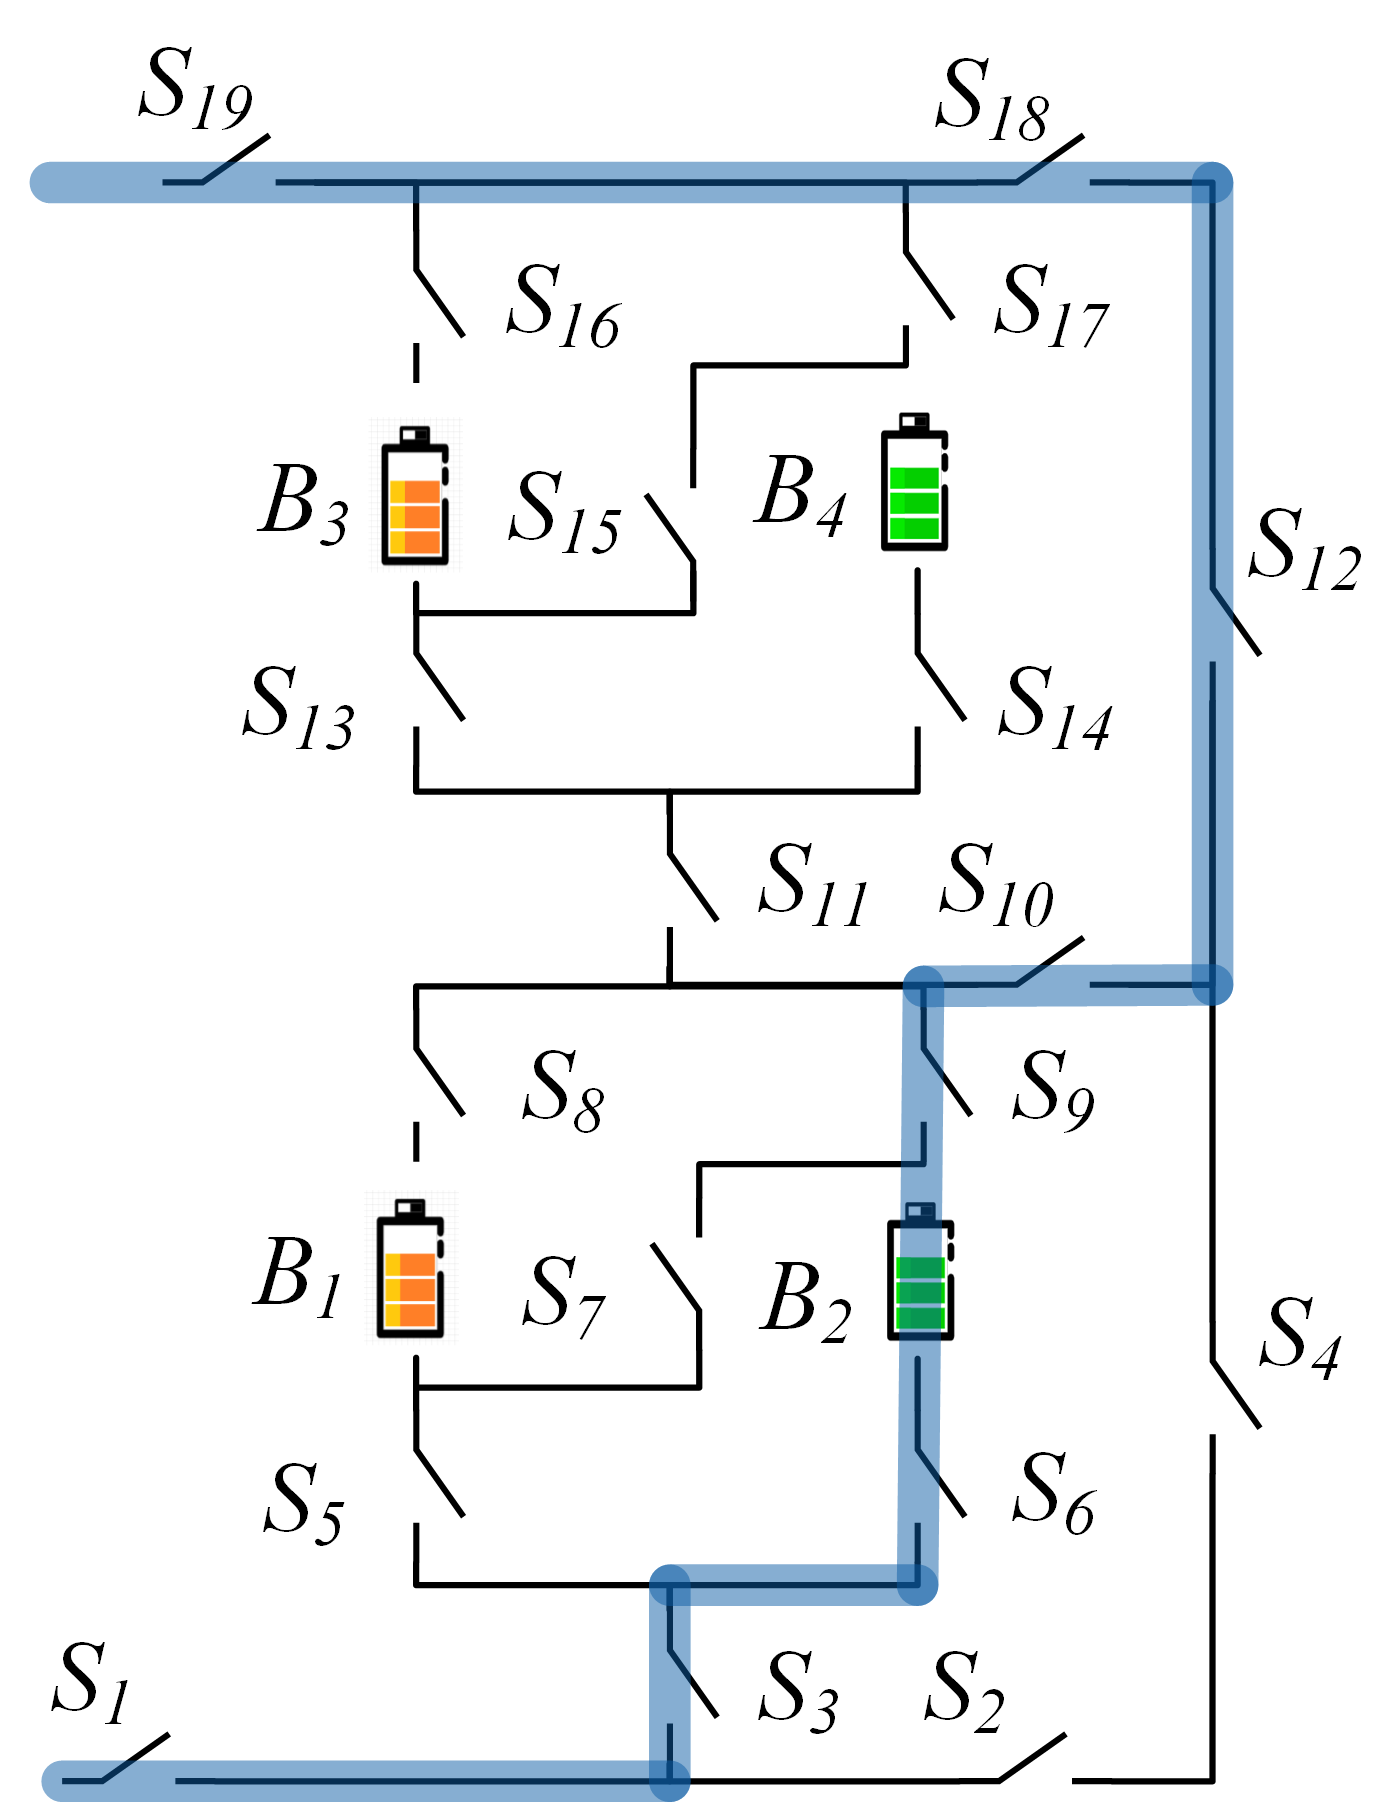
\includegraphics[width=\textwidth]{e2f2-isolate-2w.png}
        \DIFaddendFL \caption{}
        \label{fig:my-isolated-2w}
    \end{subfigure}
    \hspace{0.02\textwidth}
    \begin{subfigure}[b]{0.31\textwidth}
        \DIFdelbeginFL %DIFDELCMD < 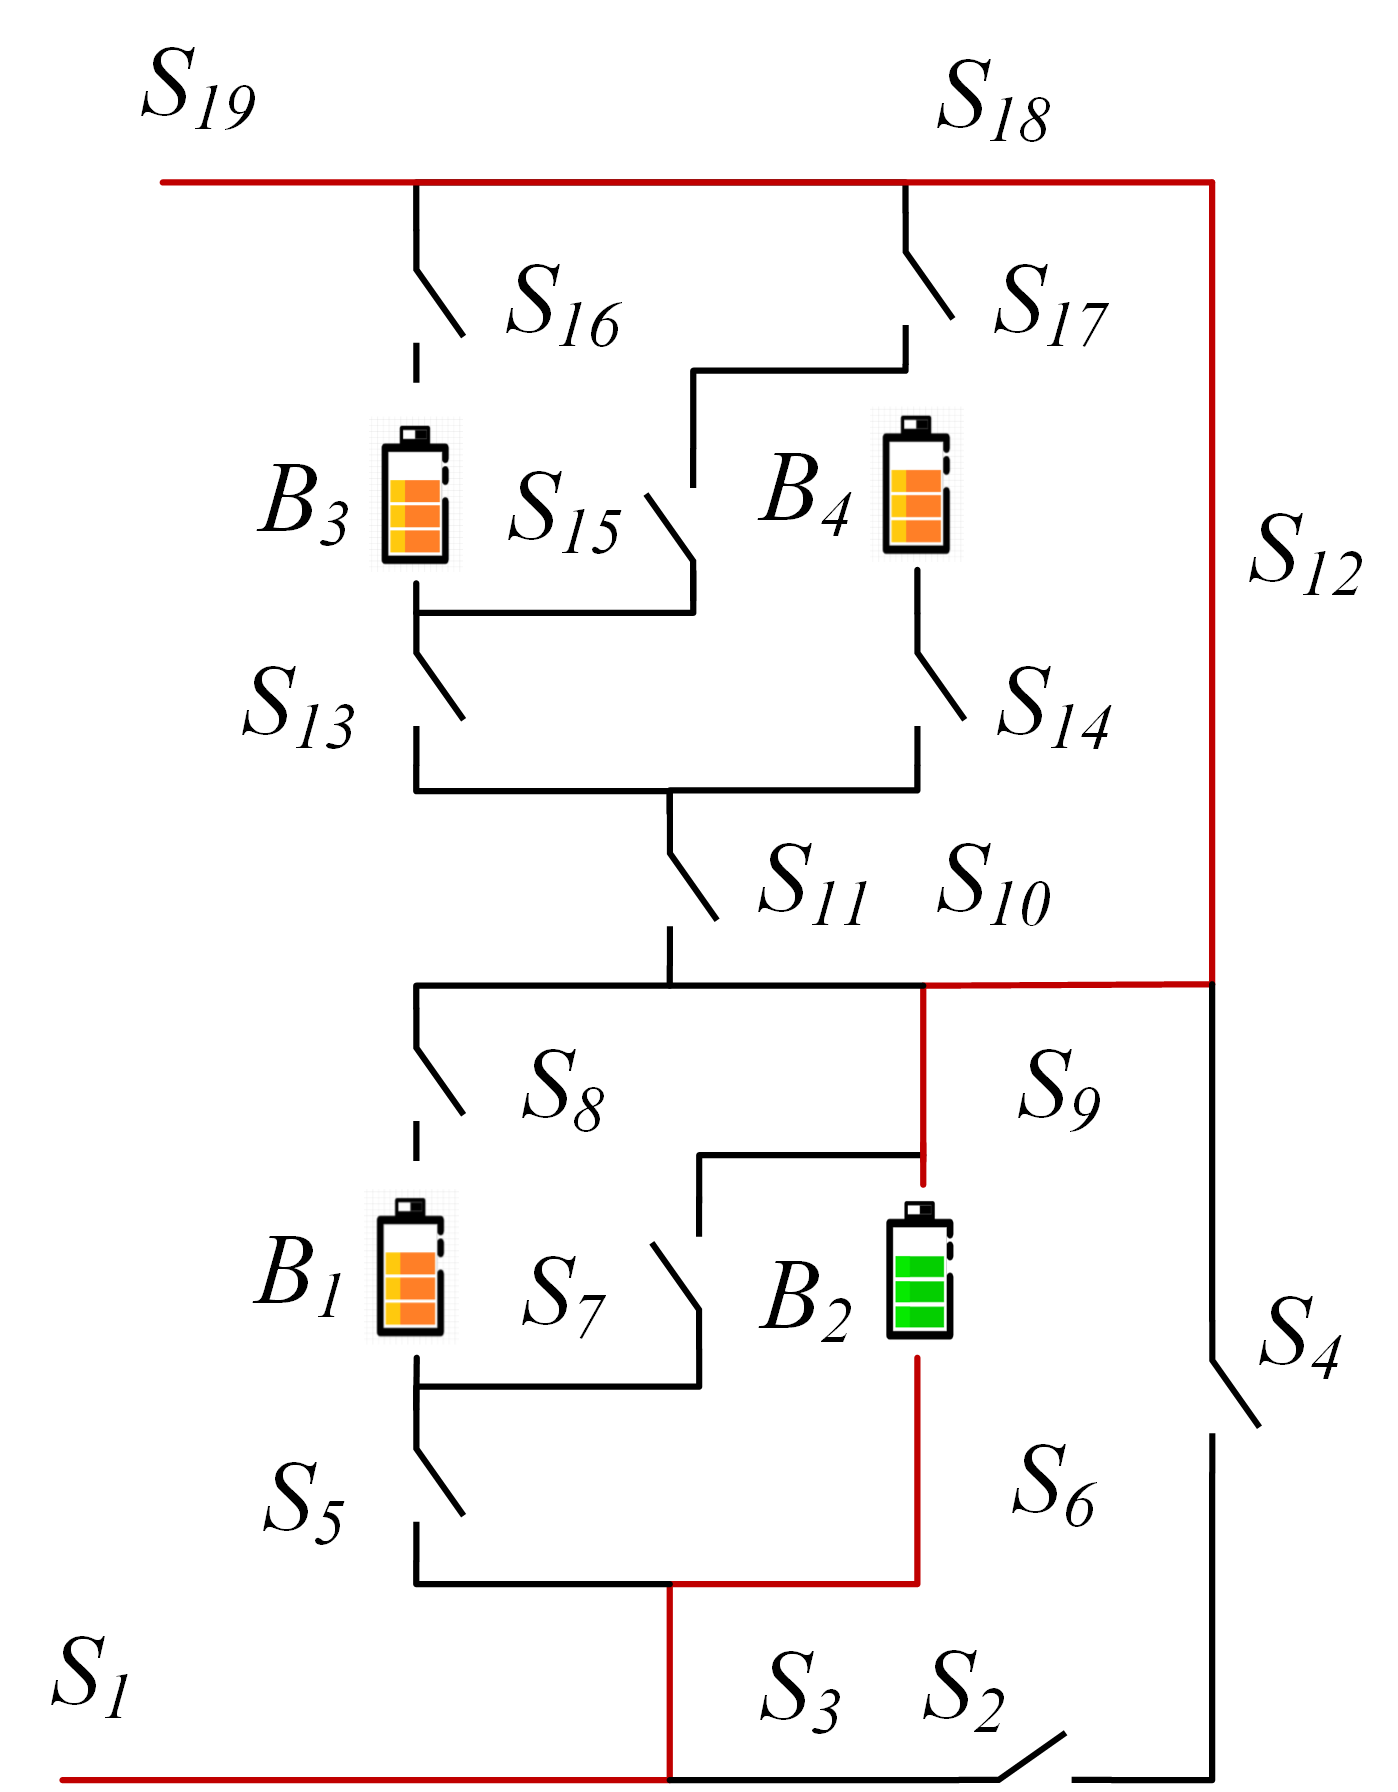
\includegraphics[width=\textwidth]{my-isolated-3.png}
%DIFDELCMD <           %%%
\DIFdelendFL \DIFaddbeginFL 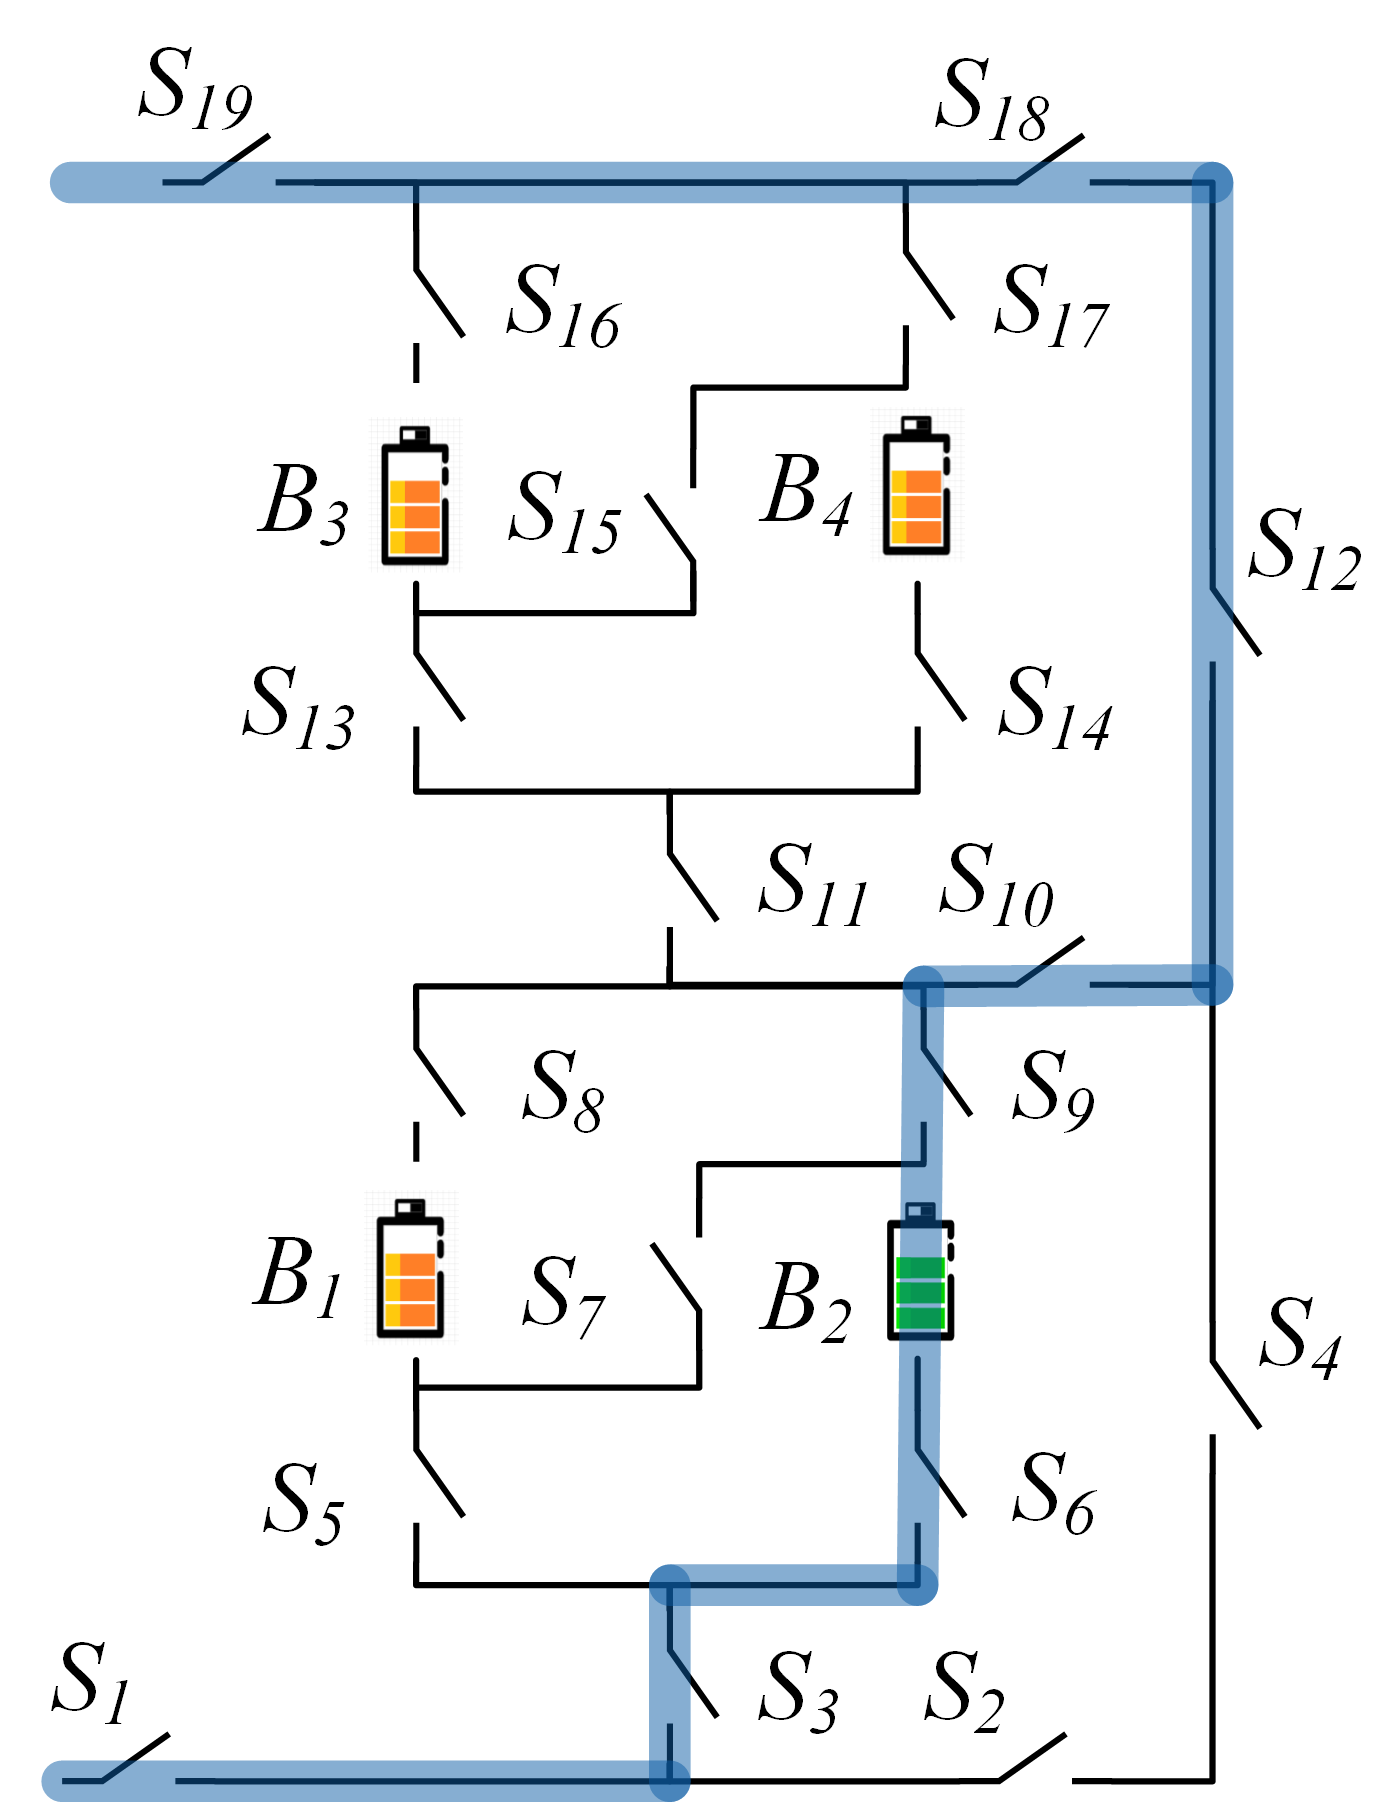
\includegraphics[width=\textwidth]{e2f2-isolate-3.png}
        \DIFaddendFL \caption{}
        \label{fig:my-isolated-3}
    \end{subfigure}
    \caption{
        \DIFdelbeginFL \DIFdelFL{Circuit }\DIFdelendFL \DIFaddbeginFL \DIFaddFL{The circuit }\DIFaddendFL states of MACs when isolating (a) one, (b) two (\DIFdelbeginFL \DIFdelFL{best case}\DIFdelendFL \DIFaddbeginFL \DIFaddFL{in different substructures}\DIFaddendFL ), (c) two (\DIFdelbeginFL \DIFdelFL{worst case}\DIFdelendFL \DIFaddbeginFL \DIFaddFL{in the same substructure}\DIFaddendFL ), and (d) three batteries for the structure in Fig. \ref{fig:study-stru-my}.
        }
\end{figure}

\subsection{Discussion}

\DIFdelbegin \DIFdel{Consider first the results }\DIFdelend \DIFaddbegin \subsubsection{\DIFadd{Result validation}}

%DIF > <*reviewer1-comment2>
\DIFadd{The correctness of the outcomes provided by the proposed greedy algorithm will now be discussed from two perspectives: circuit analysis and validation against the brute-force algorithm. 
The result of the four-battery RBS structure }\DIFaddend shown in Fig. \DIFdelbegin \DIFdel{\ref{fig:study-results-my} and listed in Tab.
\ref{tab:study-results-my}.
}\DIFdelend \DIFaddbegin \DIFadd{\ref{fig:study-stru-my} is determined as an example.
}\DIFaddend When $B_1$ and $B_2$ or $B_3$ and $B_4$ are connected in parallel, the RBS \DIFdelbegin \DIFdel{outputs }\DIFdelend \DIFaddbegin \DIFadd{produces }\DIFaddend the maximum current, which is $\eta=2$ (i.e., twice the current output of a single battery in the RBS). 
Adding more batteries to the main circuit only \DIFdelbegin \DIFdel{forms }\DIFdelend \DIFaddbegin \DIFadd{creates }\DIFaddend a series structure and does not improve the MAC. 
Therefore, the \DIFdelbegin \DIFdel{state of the switches given }\DIFdelend \DIFaddbegin \DIFadd{switch-control scheme provided }\DIFaddend in Tab. \ref{tab:study-results-my} maximizes the RBS output current.
The brute-force method, which \DIFdelbegin \DIFdel{go through }\DIFdelend \DIFaddbegin \DIFadd{examines }\DIFaddend all possible switch states, \DIFdelbegin \DIFdel{also gives the same result.
}\DIFdelend \DIFaddbegin \DIFadd{yields the same $\eta$.
This indicates that the proposed greedy algorithm successfully identifies the MAC among all the potential reconfigured structures.
%DIF > </reviewer1-comment2>
}\DIFaddend 

%DIF < <*reviewer1-comment4>
\DIFdelbegin \DIFdel{The literature contains no report on an algorithm for calculating the MAC of an RBS.
The }\DIFdelend \DIFaddbegin \subsubsection{\DIFadd{Pros and cons analysis}}

\DIFadd{The proposed greedy algorithm possesses a significant advantage in terms of its effectiveness and efficiency. 
In this paper, it is compared with the }\DIFaddend brute-force algorithm, \DIFdelbegin \DIFdel{which goes through }\DIFdelend \DIFaddbegin \DIFadd{SA, and GA. 
While the brute-force algorithm ensures the correctness of the results by exploring }\DIFaddend all possible switch states, \DIFdelbegin \DIFdel{is the most straightforward way to determine the MAC and is used as a benchmark for the }\DIFdelend \DIFaddbegin \DIFadd{it comes at a high computational cost. 
The SA and GA are commonly used heuristic algorithms for addressing NP-hard problems. 
They selectively generate solutions for the switching states to maximize the objective value $\eta$.
However, neither of these two algorithms can determine whether the current $\eta$ represents the final MAC or if there are better solutions. 
Moreover, as depicted in Figs. \ref{fig:e4-alg}--\ref{fig:e2f2-alg} and Figs. \ref{fig:e2f1-alg}--\ref{fig:e2f3-alg}, the SA and GA algorithms require more iterations to converge to the final solution than the }\DIFaddend proposed greedy algorithm. 
\DIFaddbegin 


\DIFadd{To further elaborate on the efficiency of our algorithm, we analyze the time complexity of both the brute-force algorithm and the greedy algorithm.
}\DIFaddend If an RBS has $N_b$ batteries and $N_s$ switches and the corresponding directed graph has $N$ nodes, $2^{N_s}$ iterations are required to traverse all \DIFdelbegin \DIFdel{reconfigured }\DIFdelend \DIFaddbegin \DIFadd{possible }\DIFaddend structures.
Calculating each reconfigured structure using Eqs. (\ref{eq:I_o})--(\ref{eq:eta}) requires matrix inversion and matrix multiplication, which \DIFdelbegin \DIFdel{has }\DIFdelend \DIFaddbegin \DIFadd{results in }\DIFaddend a time complexity of $O(N^3+2N^2N_b+N^2N_s+NN^2_b)$.
Therefore, the time complexity of the brute-force algorithm is $O\bm((N^3+2N^2N_b+N^2N_s+NN^2_b)2^{N_s}\bm)$.
The greedy algorithm proposed in this paper requires that \DIFaddbegin \DIFadd{the }\DIFaddend SP be found for each battery, which requires $N_b$ iterations.
Each SP can be obtained \DIFdelbegin \DIFdel{by }\DIFdelend \DIFaddbegin \DIFadd{through }\DIFaddend several applications of Dijkstra's algorithms.
Therefore, the total time complexity for calculating all SPs is $O\bm(N_b(N_b+2N_s)\log_{10} N\bm)$.
According to Appendix \ref{alg:greedy}, the RBS can reconfigure $C^{N_{\text{set}}}_{N_b}$ structures by selecting $N_{\text{set}}$ batteries from $N_b$ batteries, which gives $\sum^{N_b}_{N_{\text{set}}=1}C^{N_{\text{set}}}_{N_b}/N_b \approx 2^{N_b} N_b^{-1}$ on average.
Thus, with the bisection method, the time complexity of the greedy algorithm is $O\bm((N^3+2N^2N_b+N^2N_s+NN^2_b) 2^{N_b} N_b^{-1} \log_{10} N_b+N_b(N_b+2N_s)\log_{10} N\bm)$.
\DIFdelbegin \DIFdel{Based on currently proposed RBS structures }\DIFdelend \DIFaddbegin \DIFadd{For the existing RBS structures in the literature }\DIFaddend \cite{ciNovelDesignAdaptive2007,alahmadBatterySwitchArray2008,kimDependableEfficientScalable2010b,kimBalancedReconfigurationStorage2011a,taesickimSeriesconnectedSelfreconfigurableMulticell2012a,6843711}, the number \DIFdelbegin \DIFdel{$N_b$ of batteries , $N_s$ of switches , and $N$ of nodes }\DIFdelend \DIFaddbegin \DIFadd{of batteries $N_b$, the number of switches $N_s$, and the number of nodes $N$ }\DIFaddend are quantitatively related as follows: $N_s \approx (3\text{--} 5)N_b$, $N \approx N_s$. 
After simplifying, the time complexity of the method with \DIFaddbegin \DIFadd{the }\DIFaddend greedy algorithm is $O(2^{N_b}N_s^2\log_{10} N_b)$, while \DIFdelbegin \DIFdel{it is $O(2^{N_s}N_s^3)$ for }\DIFdelend \DIFaddbegin \DIFadd{that of }\DIFaddend the method with \DIFdelbegin \DIFdel{brute force algorithm }\DIFdelend \DIFaddbegin \DIFadd{the brute-force algorithm is $O(2^{N_s}N_s^3)$}\DIFaddend .
Therefore, as the RBS grows, especially in \DIFaddbegin \DIFadd{terms of }\DIFaddend the number of switches, the greedy algorithm gains an advantage over the brute-force algorithm.
This is confirmed by the number of structures required to determine the MAC in the previous section. 
Compared with the brute-force algorithm, the method based on the greedy algorithm is 3\,000 to 48\,000 times more efficient, which is theoretically $N_s 2^{N_s - N_b} \log_{10} N_b$ times according to the above time-complexity analysis.
This \DIFdelbegin \DIFdel{benefits from two key points}\DIFdelend \DIFaddbegin \DIFadd{is the result of two key factors}\DIFaddend :
\begin{enumerate}
    \item[(1)] The SPs guide the RBS to reconfigure reasonable structures rather than blindly going through all possible structures. This reduces the complexity from $2^{N_s}$ to $2^{N_b}$, which is the main reason for the improvement in efficiency. 
    \item[(2)] The bisection method further accelerates this process, reducing the complexity from $2^{N_b}$ to $2^{N_b} N_B^{-1} \log_{10} N_b$.
\end{enumerate}
%DIF < </reviewer1-comment4>
%DIF < <*reviewer1-comment5>
\DIFdelbegin \DIFdel{However, the greedy algorithm proposed in this paper still contains }\DIFdelend \DIFaddbegin 


\DIFadd{Furthermore, this approach can handle RBSs with arbitrary structures, which is another significant advantage. 
It can even do this when they have different battery variations or even random isolated batteries. 
Theoretically, each RBS structure can be transformed into a unique directed graph model using the methodology described in Section II, and the MAC can subsequently be calculated using the proposed greedy algorithm.
This finding is supported by the findings in the previous subsection. 
}


\DIFadd{However, the suggested greedy algorithm still includes }\DIFaddend exponential terms in \DIFdelbegin \DIFdel{the }\DIFdelend \DIFaddbegin \DIFadd{its }\DIFaddend time complexity, \DIFdelbegin \DIFdel{which means it may not be able to handle extremely large RBS structures having large $N_b$.
%DIF < </reviewer1-comment5>
}\DIFdelend \DIFaddbegin \DIFadd{indicating that it struggles to perform at scale. 
Additionally, all batteries are assumed to be identical for the sake of simplification in the derivation.
However, in reality, there may exist a small balancing current that could introduce a minor bias in the MAC due to variations in the open-circuit voltage $u_b$ and the internal resistance $r_b$.
Nevertheless, the proposed greedy algorithm remains a viable choice for RBS design and optimization in the early stage, and the issue of balancing current bias can be addressed by considering the inconsistency between batteries and replacing the internal resistance with impedance when constructing the directed graph model.
}\DIFaddend 

\DIFaddbegin \subsubsection{\DIFadd{Application scenarios}}

\DIFaddend Note that $\eta$ is used as the objective function instead of $I_o$ in solving for the MAC. 
This choice makes the resulting MAC more reasonable \DIFaddbegin \DIFadd{and applicable to practical scenarios}\DIFaddend . 
As shown in Tab. \ref{tab:study-results-my}, $I_o$ and $\bm{I}_b$ are functions of $R_o$, $u_b$, and $r_b$. 
However, when $I_o$ is used as the objective function, even for the same RBS structure, the MAC solution and corresponding switch states \DIFdelbegin \DIFdel{could }\DIFdelend \DIFaddbegin \DIFadd{can }\DIFaddend change due to different external electrical appliances.
This \DIFdelbegin \DIFdel{would increase }\DIFdelend \DIFaddbegin \DIFadd{increases }\DIFaddend the difficulty and uncertainty \DIFdelbegin \DIFdel{of }\DIFdelend \DIFaddbegin \DIFadd{involved in }\DIFaddend designing the RBS structure. 
To eliminate this problem, the ratio \DIFdelbegin \DIFdel{$\eta=I_o/\max\bm{I}_b$ }\DIFdelend \DIFaddbegin \DIFadd{$\eta=I_o/\max(\bm{I}_b)$ }\DIFaddend is adopted as the objective function in our research.
Recall that $\eta$ reflects only the structure's ability to output current, rather than the actual current \DIFdelbegin \DIFdel{outputing }\DIFdelend \DIFaddbegin \DIFadd{output }\DIFaddend by the battery system.
Assuming that the MAC of \DIFaddbegin \DIFadd{the }\DIFaddend batteries in the RBS is $I_m$, the maximum output current of the RBS structure can be calculated as $\eta I_m$ by determining the value of $\eta$ for the structure. 


The method proposed in this paper facilitates the design of RBSs in the following ways\DIFdelbegin \DIFdel{:
Most currently proposed }\DIFdelend \DIFaddbegin \DIFadd{.
Most of the existing }\DIFaddend RBS structures \cite{ciNovelDesignAdaptive2007,alahmadBatterySwitchArray2008,kimDependableEfficientScalable2010b,kimBalancedReconfigurationStorage2011a,taesickimSeriesconnectedSelfreconfigurableMulticell2012a,6843711} have simple topological characteristics, so calculating \DIFdelbegin \DIFdel{the }\DIFdelend \DIFaddbegin \DIFadd{their }\DIFaddend MACs is relatively straightforward \DIFdelbegin \DIFdel{, }\DIFdelend \DIFaddbegin \DIFadd{or }\DIFaddend even intuitive.
However, these simple structures do not always fully satisfy the requirements of complex applications, such as dynamically adapting the circuit to variable and random operating conditions or actively equalizing differences between batteries in the RBS.
Moreover, isolating the batteries disrupts the original regularity and symmetry of the topology, which complicates the otherwise simple structure, and the maximum output current of the system becomes more challenging to obtain.
In contrast, the proposed method calculates the MAC of arbitrary RBS structures, \DIFdelbegin \DIFdel{notably the }\DIFdelend \DIFaddbegin \DIFadd{most notably }\DIFaddend complex and flexible RBS structures.


To illustrate this point, the MACs of \DIFdelbegin \DIFdel{three RBS structures mentioned above }\DIFdelend \DIFaddbegin \DIFadd{the RBS structure in Fig. \ref{fig:study-stru-my} }\DIFaddend are calculated after isolating one or more of the batteries, as shown in \DIFdelbegin \DIFdel{Tab. \ref{tab:isolated_mac}. 
Specifically, for the structure presented in Fig. \ref{fig:study-stru-my}, the corresponding circuit states for the MACs when isolating one to three batteries are depicted in }\DIFdelend Figs. \ref{fig:my-isolated-1}--\ref{fig:my-isolated-3}. 
\DIFdelbegin \DIFdel{This structure has two cases in which two }\DIFdelend \DIFaddbegin \DIFadd{When a single battery is isolated, the RBS is still capable of outputting the maximum current, denoted as $\eta=2$.
When two }\DIFaddend batteries are isolated\DIFaddbegin \DIFadd{, there are two scenarios}\DIFaddend : 
one is \DIFdelbegin \DIFdel{to isolate }\DIFdelend \DIFaddbegin \DIFadd{isolating }\DIFaddend two batteries within the same substructure (Fig. \ref{fig:my-isolated-2b}), \DIFdelbegin \DIFdel{in which case }\DIFdelend \DIFaddbegin \DIFadd{resulting in }\DIFaddend $\eta=2$; the other is \DIFdelbegin \DIFdel{to isolate }\DIFdelend \DIFaddbegin \DIFadd{isolating }\DIFaddend one battery in each of the two substructures (Fig. \ref{fig:my-isolated-2w}), \DIFdelbegin \DIFdel{in which case }\DIFdelend \DIFaddbegin \DIFadd{resulting in }\DIFaddend $\eta=1$. 
\DIFdelbegin \DIFdel{The results in Figs. \ref{fig:my-isolated-1}--\ref{fig:my-isolated-3} show that the proposed method provides reasonable outcomes for isolating any number of batteries in any position.
Furthermore, the output current for the three RBSs with isolated batteries is also shown in Tab. \ref{tab:isolated_mac}. 
For the structure proposed by Lawson et al., the MAC is independent of the number of isolated batteries.
However, for Visairo's structure, the MAC decreases upon increasing the number of isolated batteries. 
Nevertheless, the MAC of the structure proposed in this work falls between the MACs of these two structures. 
This result indicates that the structure proposed in this paper has a larger MAC than Lawson's for the same number of batteriesand has a wider range of regulation of the output current}\DIFdelend \DIFaddbegin \DIFadd{If three batteries are isolated, the RBS can only output the current of a single battery, which is $\eta=1$.
Therefore, the battery management system can adjust the output current and control the RBS to reconfigure the corresponding structure based on the isolated batteries}\DIFaddend .


\section{Conclusion}

This paper \DIFdelbegin \DIFdel{proposes a pervasive }\DIFdelend \DIFaddbegin \DIFadd{has proposed a reliable }\DIFaddend and automated method to efficiently compute the MAC of an RBS.
The method is implemented \DIFdelbegin \DIFdel{by }\DIFdelend \DIFaddbegin \DIFadd{using }\DIFaddend a greedy algorithm combined with an improved directed graph model.
Not only does the method \DIFdelbegin \DIFdel{provides }\DIFdelend \DIFaddbegin \DIFadd{provide }\DIFaddend the same global MAC calculation results as the \DIFdelbegin \DIFdel{brute force }\DIFdelend \DIFaddbegin \DIFadd{brute-force }\DIFaddend method, but it also \DIFdelbegin \DIFdel{improves the calculation efficiency by 3\,000 to 48\,000 times for three RBS structures in the case study}\DIFdelend \DIFaddbegin \DIFadd{demonstrates superior computational efficiency to both the brute-force algorithm and the heuristic algorithms (SA and GA)}\DIFaddend . 
Theoretically, for an RBS with $N_s$ switches and $N_b$ batteries, the efficiency of the proposed method is $N_s 2^{N_s - N_b} \log_{10} N_b$ times that of the brute-force method\DIFdelbegin \DIFdel{, which is mainly because of using }\DIFdelend \DIFaddbegin \DIFadd{. 
This is primarily due to the utilization of }\DIFaddend the batteries' SPs \DIFdelbegin \DIFdel{to guide }\DIFdelend \DIFaddbegin \DIFadd{guiding }\DIFaddend the RBS to reconfigure reasonable structures rather than blindly going through all possible structures.
\DIFdelbegin \DIFdel{The main }\DIFdelend \DIFaddbegin \DIFadd{Another }\DIFaddend advantage of this method is its \DIFdelbegin \DIFdel{ability }\DIFdelend \DIFaddbegin \DIFadd{capability }\DIFaddend to calculate the \DIFdelbegin \DIFdel{MAC }\DIFdelend \DIFaddbegin \DIFadd{MACs }\DIFaddend of RBSs with arbitrary structures \DIFaddbegin \DIFadd{and varying batteries}\DIFaddend . 
Even in scenarios with random isolated batteries, the proposed method remains effective.
This method \DIFdelbegin \DIFdel{helps to fully tap the current output potential }\DIFdelend \DIFaddbegin \DIFadd{can facilitate the full utilization }\DIFaddend of the RBS\DIFaddbegin \DIFadd{'s current output potential}\DIFaddend , guide the \DIFdelbegin \DIFdel{RBS structure }\DIFdelend design and optimization \DIFdelbegin \DIFdel{in the design stage}\DIFdelend \DIFaddbegin \DIFadd{of the RBS structure}\DIFaddend , and assist in evaluating the \DIFdelbegin \DIFdel{current-overload risk of the system }\DIFdelend \DIFaddbegin \DIFadd{risk of current overload }\DIFaddend in practical applications.

\section{Appendix} 

\begin{algorithm}
    \caption{\DIFdelbegin \DIFdel{Get }\DIFdelend \DIFaddbegin \DIFadd{Obtain }\DIFaddend the \DIFdelbegin \DIFdel{max }\DIFdelend \DIFaddbegin \DIFadd{maximum }\DIFaddend available \DIFdelbegin \DIFdel{currents }\DIFdelend \DIFaddbegin \DIFadd{current (MAC) }\DIFaddend of a \DIFdelbegin \DIFdel{certain }\DIFdelend \DIFaddbegin \DIFadd{given }\DIFaddend RBS}\label{alg:greedy}
    \KwData{Directed graph model $G(V,E)$ of the RBS}
    \KwResult{$\max \eta$}
    \For{$i \in E_b$}{
        $P_i \leftarrow \{path| \text{starts at $v_1$ and ends at $v_n$} \}$\;
        $SP_i \leftarrow p_i \text{ which has the minimum}~\omega(p_i)~\text{among all}~p_i \in P_i. $
    }
    \DIFdelbegin \DIFdel{get }\DIFdelend \DIFaddbegin \DIFadd{Get }\DIFaddend $\bm{A}$ by Eq. \ref{eq:A}\;
    \DIFdelbegin %DIFDELCMD < \While{not yet determine $\max \eta$ }
%DIFDELCMD <     %%%
\DIFdelend \DIFaddbegin \While{not yet determined $\max \eta$ }
    \DIFaddend {
        $N_{\text{set}} \leftarrow$ number of \DIFdelbegin \DIFdel{setected }\DIFdelend \DIFaddbegin \DIFadd{selected }\DIFaddend SPs calculated by dichotomy\;
        $C_b    \leftarrow$ set of all combinations of $N_{\text{set}} $~batteries from $N_b$\;
        \DIFdelbegin %DIFDELCMD < \For{$c_b \in C_b$}{
%DIFDELCMD <             $\bm{x}_s \leftarrow \text{list of all switches' state: $x_s[j]=1$ if $ j \in \bigcup_{i\in c_b}SP_i $ else 0}$\;
%DIFDELCMD <             $\bm{X} \leftarrow diag[1,1,\cdots,1,\bm{x}_s] $\;
%DIFDELCMD <             get $\bm{Y}_n$ by Eq. \ref{eq:Yn}\;
%DIFDELCMD <             \eIf{$\bm{Y}_n$ is invertible}{
%DIFDELCMD <               pass
%DIFDELCMD <             }{construct an effective solution}
%DIFDELCMD <             get $I_o$ by Eq. \ref{eq:I_o}\;
%DIFDELCMD <             get $\bm{I}_b$ by Eq. \ref{eq:I_b}\;
%DIFDELCMD <             \eIf{$\max(\bm{I}_b)\leq I_m$}{
%DIFDELCMD <                 $\eta \leftarrow I_o/\max(\bm{I}_b)$\;
%DIFDELCMD <             }{break}
%DIFDELCMD <         }
%DIFDELCMD <     %%%
\DIFdelend \DIFaddbegin \For{$c_b \in C_b$}{
            $\bm{x}_s \leftarrow \text{list of all switches' states: $x_s[j]=1$ if $ j \in \bigcup_{i\in c_b}SP_i $ else 0}$\;
            $\bm{X} \leftarrow diag[1,1,\cdots,1,\bm{x}_s] $\;
            get $\bm{Y}_n$ by Eq. \ref{eq:Yn}\;
            \eIf{$\bm{Y}_n$ is invertible}{pass}{construct an effective solution}
            get $I_o$ by Eq. \ref{eq:I_o}\;
            get $\bm{I}_b$ by Eq. \ref{eq:I_b}\;
            \eIf{$\max(\bm{I}_b)\leq I_m$}{$\eta \leftarrow I_o/\max(\bm{I}_b)$\;}{break}
        }
    \DIFaddend }
\end{algorithm}
% \begin{figure}[htbp]
%     \centering
%     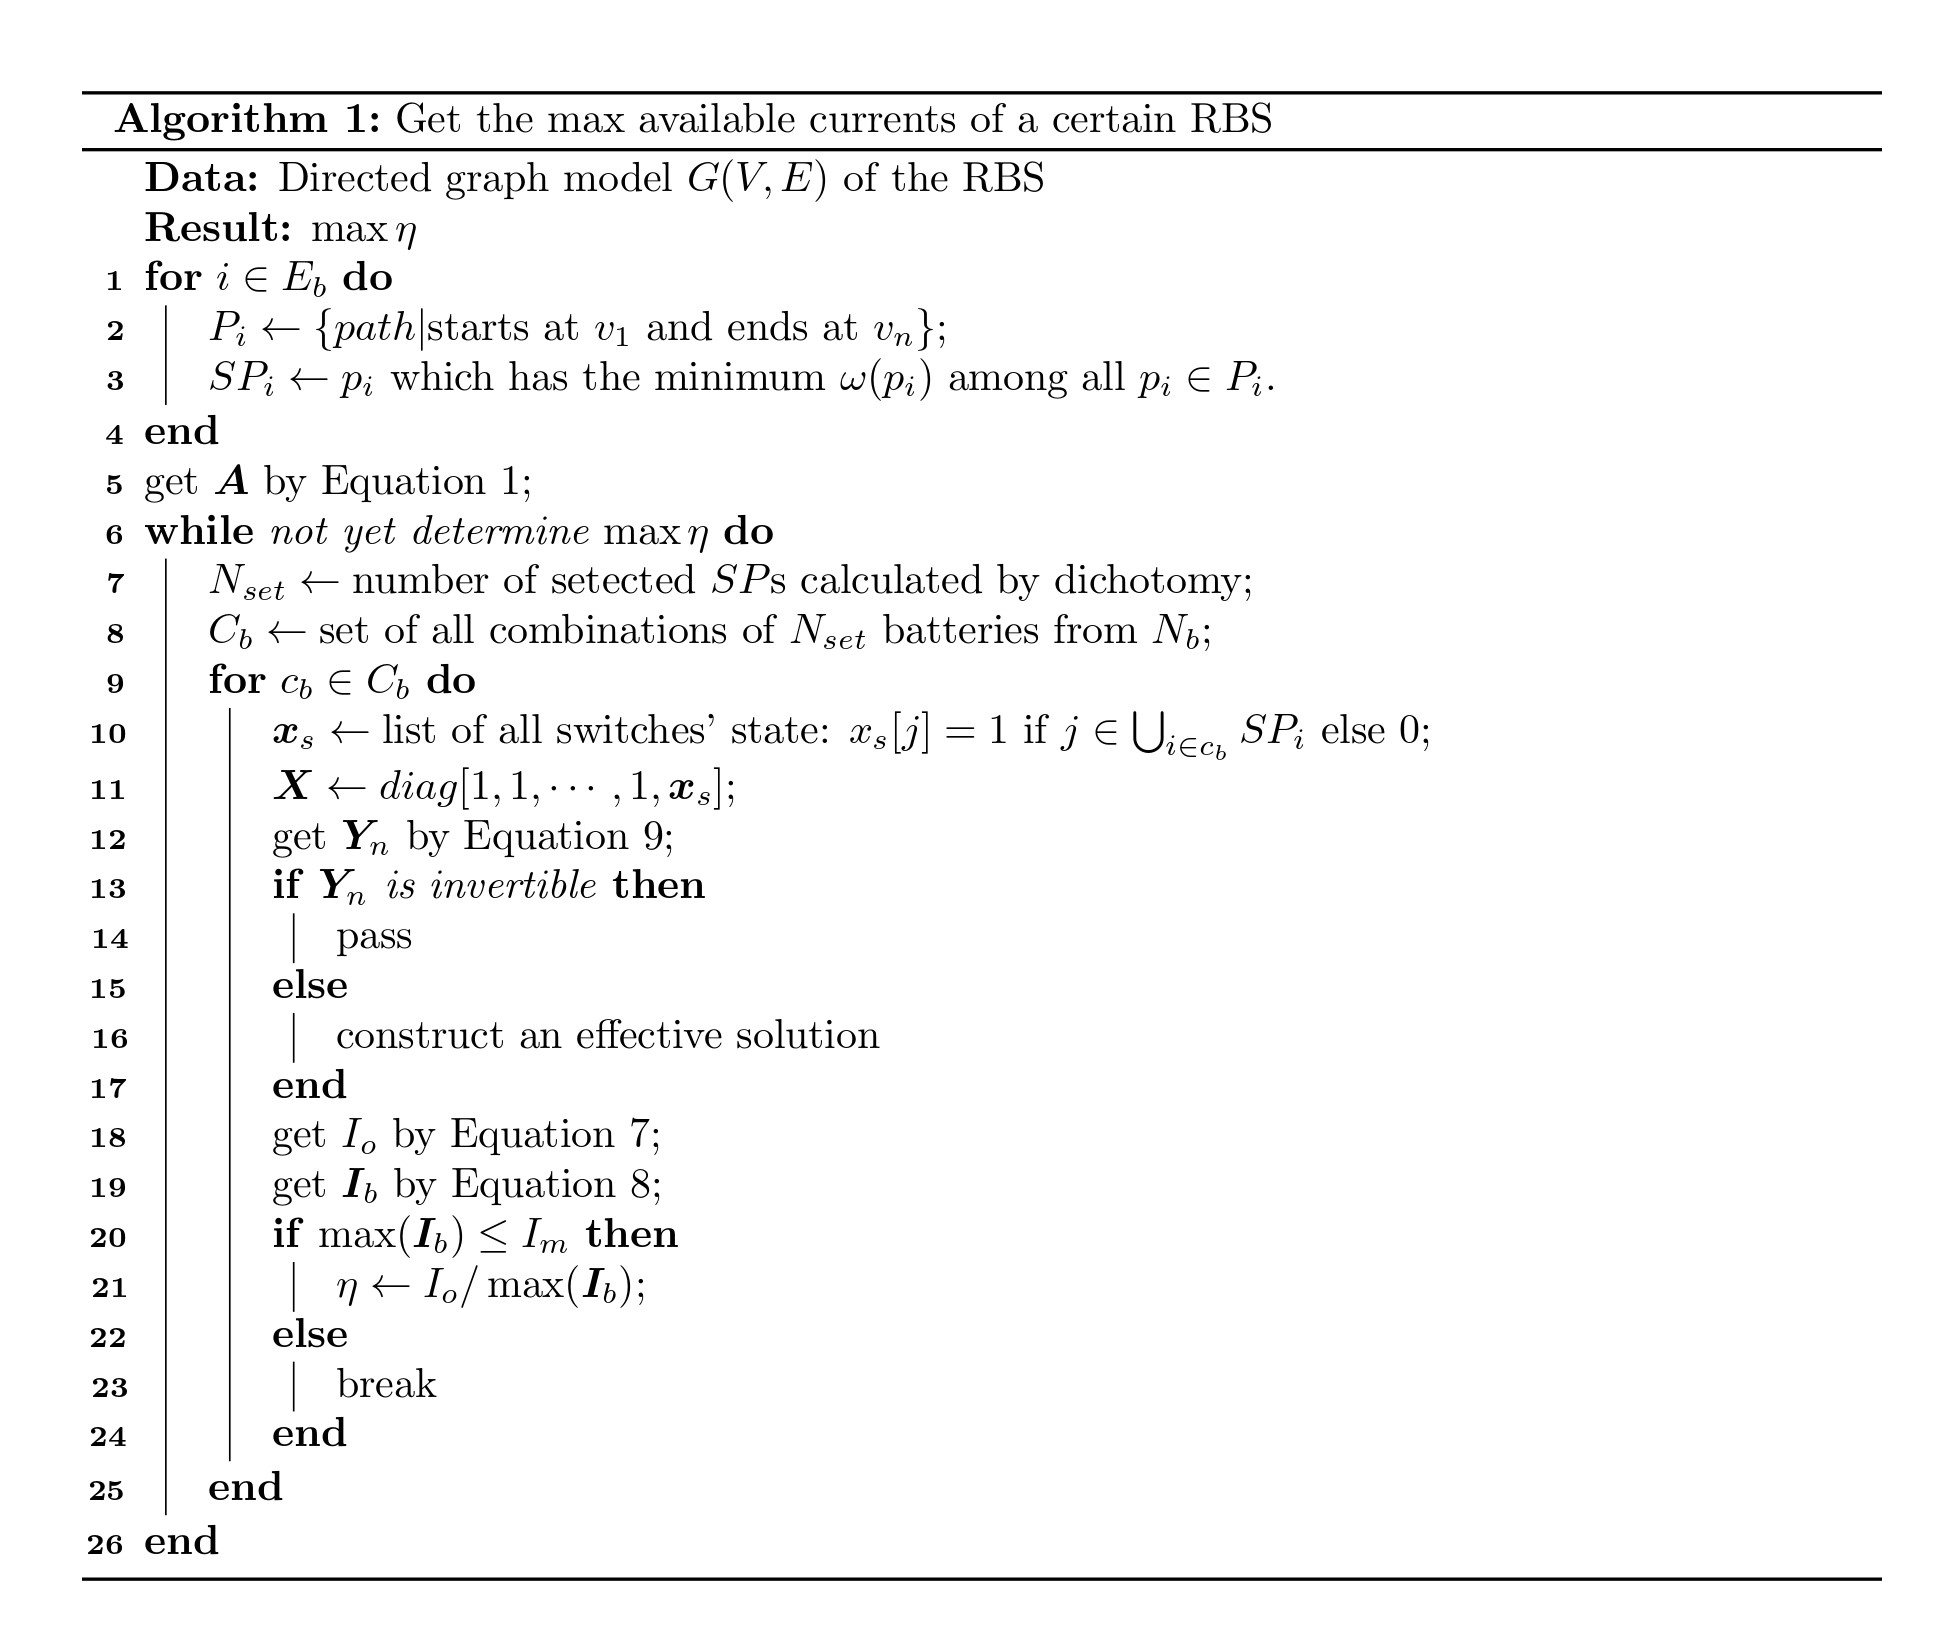
\includegraphics[width=\textwidth]{algorithm.jpg}
% \end{figure}


\section*{Acknowledgments}

\subsection*{Author Contributions} 

B. Xu conceived the main idea, formulated the overarching research goals and aims, designed the algorithm, and reviewed and revised the manuscript.
G. Hua developed and analyzed the model, implemented the code and supporting algorithms, and wrote the initial draft.
C. Qian provided critical review, commentary, and revisions.
Q. Xia contributed to shaping the research, analysis, and manuscript.
B. Sun conducted the research and investigation process.
Y. Ren secured the funding and supervised the project.
Z. Wang verified the results and provided necessary resources.

\DIFdelbegin \subsection*{\DIFdel{Funding}}
%DIFAUXCMD
%DIFDELCMD < 

%DIFDELCMD < %%%
\DIFdel{This work was supported by the National Natural Science Foundation of China (NSFC, No.52075028).
}\DIFdelend %DIF >  \subsection*{Funding}
%DIF >  
%DIF >  This work was supported by the National Natural Science Foundation of China (NSFC, No.52075028).

\subsection*{Conflicts of Interest}

The authors declare that there is no conflict of interest regarding the publication of this article.

\subsection*{Data Availability}

This work does not require any data to be declared or publicly disclosed.

\bibliographystyle{unsrt}
\bibliography{ref}

% \begin{thebibliography}{10}
% 
% \bibitem{yangBatteryEnergyStorage2018}
% Yuqing Yang, Stephen Bremner, Chris Menictas, and Merlinde Kay.
% \newblock Battery energy storage system size determination in renewable energy systems: {{A}} review.
% \newblock {\em Renewable and Sustainable Energy Reviews}, 91:109--125, August 2018.
% 
% \bibitem{desiqueiraControlStrategySmooth2021}
% Luanna Maria~Silva {de Siqueira} and Wei Peng.
% \newblock Control strategy to smooth wind power output using battery energy storage system: {{A}} review.
% \newblock {\em Journal of Energy Storage}, 35:102252, March 2021.
% 
% \bibitem{schwanbeckInternationalSpaceStation2019}
% Eugene Schwanbeck and Penni Dalton.
% \newblock International {{Space Station Lithium-ion Batteries}} for {{Primary Electric Power System}}.
% \newblock In {\em 2019 {{European Space Power Conference}} ({{ESPC}})}, pages 1--1. {IEEE}, September 2019.
% 
% \bibitem{zhangDevelopmentProspectChinese2021}
% Lihua Zhang.
% \newblock Development and {{Prospect}} of {{Chinese Lunar Relay Communication Satellite}}.
% \newblock {\em Space: Science \& Technology}, 2021, January 2021.
% 
% \bibitem{choCommercialResearchBattery2015}
% Jaephil Cho, Sookyung Jeong, and Youngsik Kim.
% \newblock Commercial and research battery technologies for electrical energy storage applications.
% \newblock {\em Progress in Energy and Combustion Science}, 48:84--101, June 2015.
% 
% \bibitem{yangUnbalancedDischargingAging2016}
% Naixing Yang, Xiongwen Zhang, BinBin Shang, and Guojun Li.
% \newblock Unbalanced discharging and aging due to temperature differences among the cells in a lithium-ion battery pack with parallel combination.
% \newblock {\em Journal of Power Sources}, 306:733--741, February 2016.
% 
% \bibitem{fengPropagationMechanismsDiagnosis2019}
% Fei Feng, Xiaosong Hu, Lin Hu, Fengling Hu, Yang Li, and Lei Zhang.
% \newblock Propagation mechanisms and diagnosis of parameter inconsistency within {{Li-Ion}} battery packs.
% \newblock {\em Renewable and Sustainable Energy Reviews}, 112:102--113, September 2019.
% 
% \bibitem{jeevarajanBatterySafetyQualifications2012}
% J.~A. Jeevarajan and C.~Winchester.
% \newblock Battery {{Safety Qualifications}} for {{Human Ratings}}.
% \newblock {\em Interface magazine}, 21(2):51--55, January 2012.
% 
% \bibitem{pomboHybridPowerSystem2021}
% Daniel~V{\'a}zquez Pombo.
% \newblock A {{Hybrid Power System}} for a {{Permanent Colony}} on {{Mars}}.
% \newblock {\em Space: Science \& Technology}, 2021, January 2021.
% 
% \bibitem{hanNextGenerationBatteryManagement2020a}
% Weiji Han, Torsten Wik, Anton Kersten, Guangzhong Dong, and Changfu Zou.
% \newblock Next-{{Generation Battery Management Systems}}: {{Dynamic Reconfiguration}}.
% \newblock {\em IEEE Industrial Electronics Magazine}, 14(4):20--31, December 2020.
% 
% \bibitem{visairoReconfigurableBatteryPack2008}
% H.~Visairo and P.~Kumar.
% \newblock A reconfigurable battery pack for improving power conversion efficiency in portable devices.
% \newblock In {\em 2008 7th {{International Caribbean Conference}} on {{Devices}}, {{Circuits}} and {{Systems}}}, pages 1--6. {IEEE}, April 2008.
% 
% \bibitem{ci2007novel}
% Song Ci, Jiucai Zhang, Hamid Sharif, and Mahmoud Alahmad.
% \newblock A novel design of adaptive reconfigurable multicell battery for power-aware embedded networked sensing systems.
% \newblock In {\em IEEE GLOBECOM 2007-IEEE Global Telecommunications Conference}, pages 1043--1047. IEEE, 2007.
% 
% \bibitem{9209774}
% Jan Engelhardt, Tatiana Gabderakhmanova, Gunnar Rohde, and Mattia Marinelli.
% \newblock Reconfigurable stationary battery with adaptive cell switching for electric vehicle fast-charging.
% \newblock In {\em 2020 55th International Universities Power Engineering Conference (UPEC)}, pages 1--6, 2020.
% 
% \bibitem{engelhardt2021double}
% Jan Engelhardt, Jan~Martin Zepter, Tatiana Gabderakhmanova, Gunnar Rohde, and Mattia Marinelli.
% \newblock Double-string battery system with reconfigurable cell topology operated as a fast charging station for electric vehicles.
% \newblock {\em Energies}, 14(9):2414, 2021.
% 
% \bibitem{lawsonSoftwareConfigurableBattery2012}
% Barrie Lawson.
% \newblock A {{Software Configurable Battery}}.
% \newblock {\em EVS26 International Battery, Hybrid and Fuel Cell Electric Vehicle Symposium}, 2012.
% 
% \bibitem{he2014reconfiguration}
% Liang He, Linghe Kong, Siyu Lin, Shaodong Ying, Yu~Gu, Tian He, and Cong Liu.
% \newblock Reconfiguration-assisted charging in large-scale lithium-ion battery systems.
% \newblock In {\em 2014 ACM/IEEE International Conference on Cyber-Physical Systems (ICCPS)}, pages 60--71. IEEE, 2014.
% 
% \bibitem{kim2009dynamic}
% Hahnsang Kim and Kang~G Shin.
% \newblock On dynamic reconfiguration of a large-scale battery system.
% \newblock In {\em 2009 15th IEEE Real-Time and Embedded Technology and Applications Symposium}, pages 87--96. IEEE, 2009.
% 
% \bibitem{han2021analysis}
% Weiji Han, Anton Kersten, Changfu Zou, Torsten Wik, Xiaoliang Huang, and Guangzhong Dong.
% \newblock Analysis and estimation of the maximum switch current during battery system reconfiguration.
% \newblock {\em IEEE Transactions on Industrial Electronics}, 69(6):5931--5941, 2021.
% 
% \bibitem{chenSneakCircuitTheory2021}
% Si-Zhe Chen, Yule Wang, Guidong Zhang, Le~Chang, and Yun Zhang.
% \newblock Sneak {{Circuit Theory Based Approach}} to {{Avoiding Short-Circuit Paths}} in {{Reconfigurable Battery Systems}}.
% \newblock {\em IEEE Transactions on Industrial Electronics}, 68(12):12353--12363, 2021.
% 
% \bibitem{heExploringAdaptiveReconfiguration2013}
% Liang He, Lipeng Gu, Linghe Kong, Yu~Gu, Cong Liu, and Tian He.
% \newblock Exploring {{Adaptive Reconfiguration}} to {{Optimize Energy Efficiency}} in {{Large-Scale Battery Systems}}.
% \newblock In {\em 2013 {{IEEE}} 34th {{Real-Time Systems Symposium}}}, pages 118--127, December 2013.
% 
% \bibitem{hongwenheStateofChargeEstimationLithiumIon2011}
% Hongwen He, Rui Xiong, Xiaowei Zhang, Fengchun Sun, and JinXin Fan.
% \newblock State-of-{{Charge Estimation}} of the {{Lithium-Ion Battery Using}} an {{Adaptive Extended Kalman Filter Based}} on an {{Improved Thevenin Model}}.
% \newblock {\em IEEE Transactions on Vehicular Technology}, 60(4):1461--1469, May 2011.
% 
% \bibitem{mousavig.VariousBatteryModels2014}
% S.M. Mousavi~G. and M.~Nikdel.
% \newblock Various battery models for various simulation studies and applications.
% \newblock {\em Renewable and Sustainable Energy Reviews}, 32:477--485, April 2014.
% 
% \bibitem{ciNovelDesignAdaptive2007}
% Song Ci, Jiucai Zhang, Hamid Sharif, and Mahmoud Alahmad.
% \newblock A {{Novel Design}} of {{Adaptive Reconfigurable Multicell Battery}} for {{Power-Aware Embedded Networked Sensing Systems}}.
% \newblock In {\em {{IEEE GLOBECOM}} 2007-2007 {{IEEE Global Telecommunications Conference}}}, pages 1043--1047, November 2007.
% 
% \bibitem{alahmadBatterySwitchArray2008}
% Mahmoud Alahmad, Herb Hess, Mohammad Mojarradi, William West, and Jay Whitacre.
% \newblock Battery switch array system with application for {{JPL}}'s rechargeable micro-scale batteries.
% \newblock {\em Journal of Power Sources}, 177(2):566--578, March 2008.
% 
% \bibitem{kimDependableEfficientScalable2010b}
% Hahnsang Kim and Kang~G. Shin.
% \newblock Dependable, efficient, scalable architecture for management of large-scale batteries.
% \newblock In {\em Proceedings of the 1st {{ACM}}/{{IEEE International Conference}} on {{Cyber-Physical Systems}}}, {{ICCPS}} '10, pages 178--187, {New York, NY, USA}, April 2010. {Association for Computing Machinery}.
% 
% \bibitem{kimBalancedReconfigurationStorage2011a}
% Younghyun Kim, Sangyoung Park, Yanzhi Wang, Qing Xie, Naehyuck Chang, Massimo Poncino, and Massoud Pedram.
% \newblock Balanced reconfiguration of storage banks in a hybrid electrical energy storage system.
% \newblock In {\em 2011 {{IEEE}}/{{ACM International Conference}} on {{Computer-Aided Design}} ({{ICCAD}})}, pages 624--631, November 2011.
% 
% \bibitem{taesickimSeriesconnectedSelfreconfigurableMulticell2012a}
% Taesic Kim, Wei Qiao, and Liyan Qu.
% \newblock A series-connected self-reconfigurable multicell battery capable of safe and effective charging/discharging and balancing operations.
% \newblock In {\em 2012 {{Twenty-Seventh Annual IEEE Applied Power Electronics Conference}} and {{Exposition}} ({{APEC}})}, pages 2259--2264, February 2012.
% 
% \bibitem{6843711}
% Liang He, Linghe Kong, Siyu Lin, Shaodong Ying, Yu~Gu, Tian He, and Cong Liu.
% \newblock Reconfiguration-assisted charging in large-scale {{Lithium-ion}} battery systems.
% \newblock In {\em 2014 {{ACM}}/{{IEEE International Conference}} on {{Cyber-Physical Systems}} ({{ICCPS}})}, pages 60--71, April 2014.
% 
% \end{thebibliography}

% \printbibliography

\end{document}
